

\documentclass[
    titlepage,
    chapterprefix=true
]{scrbook}

\usepackage{amsmath}
\usepackage{mathtools}
\usepackage[paper=a4paper, inner=2cm, outer=0.5cm, top=5cm]{geometry}
\usepackage{graphicx}
\usepackage{siunitx}
\usepackage{makeidx}
\usepackage{polyglossia}
\setdefaultlanguage[variant=uk]{english}


\usepackage[warnings-off={mathtools-colon,mathtools-overbracket}]{unicode-math}
\usepackage{fontspec}
\usepackage[
    headsepline%=1pt:\linewidth
    %footsepline=1pt:\linewidth
]{scrlayer-scrpage}
\usepackage[dvipsnames]{xcolor}
%\usepackage{titlesec}
\usepackage{multirow}
\usepackage{xcolor}
% additional header file for standalone images


\usepackage{tikz}
\usepackage{tikz-3dplot}
\usetikzlibrary{patterns, shapes}
\usepackage{pgfplots}
\pgfplotsset{compat=1.16}
\usetikzlibrary{cd}

\newcommand{\LTRIA}{0.5}
\newcommand{\triang}[2]{\filldraw[fill=#2!60!white, draw=#2!50!black, very thick] #1 -- ($ #1 + (\LTRIA, 0) $) -- ($ #1 + (0.5*\LTRIA, \LTRIA) $) -- cycle;}

\newcommand{\BZRc}{0.5519}

\newcommand{\bezierc}[2] {
  \begin{scope}[cm={#1,0,0,#1,(0,0)}]
  \draw[very thick, #2] (0,1) .. controls (\BZRc, 1) and (1,\BZRc) .. (1,0);
  \draw[very thick, #2] (1,0) .. controls (1, -\BZRc) and (\BZRc, -1) .. (0,-1);
  \draw[very thick, #2] (0,-1) .. controls (-\BZRc, -1) and (-1,-\BZRc) .. (-1,0);
  \draw[very thick, #2] (-1,0) .. controls (-1, \BZRc) and (-\BZRc,1) .. (0,1);
\end{scope}
}

\newcommand{\beziercnl}[3] {
  \begin{scope}[cm={#1,0,0,#1,(0,0)}]
    \draw[very thick, #3] (0,1.2) .. controls (\BZRc, 1.2) and ($(1,\BZRc)-(#2,0.0)$) .. (1,0);
    \draw[very thick, #3] (1,0) .. controls ($(1, -\BZRc)+(#2,0.0)$) and ($(\BZRc, -1) + (0.0,#2)$) .. (0,-1.1);
    \draw[very thick, #3] (0,-1.1) .. controls ($(-\BZRc, -1)-(0.0,#2)$) and ($(-1.2,-\BZRc)-(#2,0.0)$) .. (-1,0);
    \draw[very thick, #3] (-1,0) .. controls ($(-.8, \BZRc)+(#2,0.0)$) and (-\BZRc,1.2) .. (0,1.2);
\end{scope}
}

\newcommand{\beziercnlTwo}[4] {
  \begin{scope}[cm={#1,0,0,#1,(0,0)}]
    \coordinate (Pnorth) at ($(0, 1.2) + (0, #4)$);

    \draw[very thick, #3] (Pnorth) .. controls ($(\BZRc, 0) + (Pnorth)$) and ($(1,\BZRc)-(#2,0.0)$) .. (1,0);
    \draw[very thick, #3] (1,0) .. controls ($(1, -\BZRc)+(#2,0.0)$) and ($(\BZRc, -1) + (0.0,#2)$) .. (0,-1.1);
    \draw[very thick, #3] (0,-1.1) .. controls ($(-\BZRc, -1)-(0.0,#2)$) and ($(-1.2,-\BZRc)-(#2,0.0)$) .. (-1,0);
    \draw[very thick, #3] (-1,0) .. controls ($(-.8, \BZRc)+(#2,0.0)$) and ($(-\BZRc,0)+(Pnorth)$) .. (Pnorth);
\end{scope}
}

\usepackage[build]{standalone}
\usepackage{wrapfig}
\usepackage{setspace}
\usepackage[
    pdfencoding=auto,
    psdextra,
    colorlinks=true
]{hyperref}
\usepackage[format=hang]{caption}

\graphicspath{%
    {figures/}%
    {figures/intro/}%
    {figures/nbpm/}%
    {figures/lobster/}%
    {twiss/}%
    {forcedcoupling/}%
}
\makeindex


% debug
\usepackage{lipsum}
\newcommand{\DBGNolink}{\texttt{<no-link>}}


% --------------------------------------------------------------------------------------------------
% fontawesome
% --------------------------------------------------------------------------------------------------
\usepackage{fontawesome5}
%% Local computer
%\newfontfamily{\afont}{Font Awesome 5 Brands-Regular-400.otf}
%\newfontfamily{\awfont}{Font Awesome 5 Free-Regular-400.otf}
%\newfontfamily{\asfont}{Font Awesome 5 Free-Solid-900.otf}

% Overleaf, different font names
\newfontfamily{\afont}{FontAwesome5Brands-Regular-400.otf}
\newfontfamily{\awfont}{FontAwesome5Free-Regular-400.otf}
\newfontfamily{\asfont}{FontAwesome5Free-Solid-900.otf}

% selection of fontawesome symbols
\newcommand{\FAb}[1] {{\afont \symbol{"#1}}\hspace{.5em}}
\newcommand{\FA}[1] {{\awfont \symbol{"#1}}\hspace{.5em}}
\newcommand{\FAs}[1] {{\asfont \symbol{"#1}}\hspace{.5em}}

% --------------------------------------------------------------------------------------------------
% fonts
% --------------------------------------------------------------------------------------------------
\setmainfont{STIX Two Text}[RawFeature={+liga}]
\setmathfont{STIX Two Math}
\setsansfont{TeX Gyre Heros}



% fix phi, why do they use the ugly print face phi as standard?
\AtBeginDocument{
    \let\phi\varphi
}

% --------------------------------------------------------------------------------------------------
% page layout
% --------------------------------------------------------------------------------------------------
\clearscrheadfoot
\addtokomafont{pagenumber}{\oldstylenums}
\KOMAoptions{headsepline=false}

\definecolor{headfootsepcolor}{RGB}{200,200,200}
\addtokomafont{headsepline}{\color{headfootsepcolor}}

\ohead[\pagemark]{\pagemark}

%% print: 4.0 -- 2.5
%\newdimen{\outermarg}      \setlength{\outermarg}{2.5cm} % leave considerable outer border for images
%\newdimen{\innermarg}      \setlength{\innermarg}{4.0cm} % leave large inner border for binding
% pdf: 3.5 -- 3.0
\newdimen{\outermarg}      \setlength{\outermarg}{3.0cm} % leave considerable outer border for images
\newdimen{\innermarg}      \setlength{\innermarg}{3.5cm} % leave large inner border for binding
\newlength{\figborderhang} 
\setlength{\figborderhang}{\outermarg} % aligns images with the outer border (if placement o or O used)
\addtolength{\figborderhang}{-1.0cm} % and leaves 1cm from the border

\setlength{\belowcaptionskip}{-.8\baselineskip}
\newcommand{\textlinespread}{1.25}
\newcommand{\captionlinespread}{1.125}
\newcommand{\infolinespread}{1.125}

\captionsetup{format=plain,labelfont=bf, font={small,stretch=\captionlinespread}}


% --------------------------------------------------------------------------------------------------
% sectioning
% --------------------------------------------------------------------------------------------------
%\makeatletter
%\renewcommand{\chapterlinesformat}[3]{%
%\vspace{2em}
%    \framebox{%
%        
%        \parbox{\dimexpr\linewidth-2\fboxrule-2\fboxsep}{%
%            \vspace{1.5em}%
%            \begin{center}%
%            \Huge\normalfont\bfseries
%            \addfontfeature{Letters=SmallCaps}
%            \bfseries
%            #3%
%            \end{center}%
%            \vspace{1.5em}%
%        }%
%    }\\
%    \raisebox{0pt}[0pt][0pt]{%
%        \raisebox{5em}{%
%        \hspace{0.5em}
%        \colorbox{white}{
%            \normalfont\Large%
%            \hspace{0.5em}%
%            CHAPTER \thechapter%
%            \hspace{0.75em}%
%        }
%        }%
%    }\\
%}
%\renewcommand{\thechapter}{%
%    \normalfont \Large%
%    \hspace{0.5em}%
%    CHAPTER~\arabic{chapter}%
%    \hspace{0.75em}%
%}
\renewcommand*{\chapterformat}{%
    \normalfont \Large%
    \hspace{0.5em}%
    \MakeUppercase{\chapapp}~\thechapter%
    \hspace{0.75em}%
}

\makeatletter
\renewcommand{\chapterlineswithprefixformat}[3]{%
\begin{tikzpicture}
    \node[draw,rectangle,below right] at (0,0) {%
        \parbox{\dimexpr\linewidth-2\fboxrule-2\fboxsep}{%
            \vspace{1.5em}%
            \begin{center}%
            \Huge\normalfont\addfontfeature{Letters=SmallCaps} \bfseries
            #3%
            \end{center}%
            \vspace{1.5em}%
        }%
    };
    \Ifstr{#2}{}{}{%
        \node[fill=white,below right] at (0.5em,0.5em) {%
            \normalfont \Large%
            \hspace{0.5em}%
            \MakeUppercase{\chapapp}~\thechapter%
            \hspace{0.75em}%
        };%
    }
\end{tikzpicture}
}

\renewcommand{\chapterlinesformat}[3]{%
\begin{tikzpicture}
    \node[draw,rectangle,below right] at (0,0) {%
        \parbox{\dimexpr\linewidth-2\fboxrule-2\fboxsep}{%
            \vspace{1.0em}%
            \begin{center}%
            \Huge\normalfont\addfontfeature{Letters=SmallCaps} \bfseries
            #2~#3%
            \end{center}%
            \vspace{1.0em}%
        }%
    };
\end{tikzpicture}
}

\renewcommand{\sectionlinesformat}[4]{%
    \Ifstr{#1}{section}{%
   \normalfont\Large\bfseries #3~#4%
   }{%
   \normalfont\large\bfseries #3~#4%
   }
   
}

\makeatother

%\titleformat{\chapter}[frame]
%{\normalfont\thispagestyle{empty}\addfontfeatures{Letters=SmallCaps}}
%{\filright \hspace{1em} CHAPTER \thechapter \hspace{1em}}
%{8pt}
%{\Huge\bfseries\filcenter}
%
%\titleformat{\section}
%{\normalfont}
%{\filright\Large \bfseries \thesection \hspace{1em}}
%{8pt}
%{\Large\bfseries}
%
%\titleformat{\subsection}
%{\normalfont}
%{\filright\large \bfseries \thesubsection \hspace{1em}}
%{8pt}
%{\large\bfseries}
%
%\titleformat{\subsubsection}
%{\normalfont}
%{\filright\large \bfseries \thesubsubsection \hspace{1em}}
%{8pt}
%{\large\bfseries}

\newenvironment{chapterinfo}
{
    \hspace{1cm}\begin{minipage}{\dimexpr\textwidth-2cm}%
    \small%
    \itshape\parindent1em
    \renewcommand\baselinestretch{\infolinespread}\selectfont
}{
    \end{minipage}%
    %\vspace{1.5em}%
    \normalfont%
    \normalsize
}

% --------------------------------------------------------------------------------------------------
% my definitions
% --------------------------------------------------------------------------------------------------
\newcommand{\fstop}{\quad .}
\newcommand{\komma}{\quad ,}
\renewcommand{\eqref}[1]{Eq.~(\ref{#1})}
\newcommand{\equationref}[1]{Equation~(\ref{#1})}
\newcommand{\figref}[1]{Fig.~\ref{#1}}
\newcommand{\figureref}[1]{Figure~\ref{#1}}

\newcommand{\der}{\;\text{d}}
\newcommand{\e}[1]{\text{e}^{#1}}
\newcommand{\expi}[1]{\text{e}^{i\left(#1\right)}}
\newcommand{\m}{^\text{m}}
\newcommand{\mat}[1]{\mathbf{#1}}
\newcommand{\betastar}{\beta^*}
\newcommand{\sumw}{\sum\limits_{w \in I}}
\newcommand{\liemap}[1] {{:}#1{:}\,}
\newcommand{\liemapn}[2] {{:}#1{:}^{#2}\,}
\newcommand{\atan}{\mathrm{atan}}

\newcommand{\zxp}{\zeta_x^+}
\newcommand{\zxm}{\zeta_x^-}
\newcommand{\zyp}{\zeta_y^+}
\newcommand{\zym}{\zeta_y^-}

\newcommand{\zxpto}[1]{\left(\zeta_x^+\right)^{#1}}
\newcommand{\zxmto}[1]{\left(\zeta_x^-\right)^{#1}}
\newcommand{\zypto}[1]{\left(\zeta_y^+\right)^{#1}}
\newcommand{\zymto}[1]{\left(\zeta_y^-\right)^{#1}}

\newcommand{\hxp}{h_x^+}
\newcommand{\hxm}{h_x^-}
\newcommand{\hyp}{h_y^+}
\newcommand{\hym}{h_y^-}

\newcommand{\hxpto}[1]{\left(h_x^+\right)^{#1}}
\newcommand{\hxmto}[1]{\left(h_x^-\right)^{#1}}
\newcommand{\hypto}[1]{\left(h_y^+\right)^{#1}}
\newcommand{\hymto}[1]{\left(h_y^-\right)^{#1}}

\newcommand{\four}[1]{\mathcal{F} \left\{ #1 \right\}}
\newcommand{\conj}[1]{#1^*}

\newcommand{\ave}[2]
{
  \left\langle #1 \right\rangle_{#2}
}
\newcommand{\phiave}[1]{
  \ave{#1}{\varphi}
}



\newcommand{\re}[1]{\mathcal{Re} \left\{ #1 \right\} }
\newcommand{\im}[1]{\mathcal{Im} \left\{ #1 \right\} }

\usepackage[dvipsnames]{xcolor}
\usepackage{tikz}
\usetikzlibrary{calc}
\usepackage{siunitx}

%\usepackage{xparse}
\pgfdeclarelayer{bg}    
\pgfsetlayers{bg,main}  

\definecolor{bpmused}{RGB}{225,120,0}
\definecolor{bpmnot}{RGB}{180,180,180}
\definecolor{bar}{RGB}{50,50,50}
\definecolor{quadblue}{RGB}{50,150,255}
\definecolor{sextclr}{RGB}{250,50,255}
\definecolor{otherclr}{RGB}{10,205,100}
\newcommand{\bpmthickness}{0.15}
\newcommand{\sextheight}{0.0}
\newcommand{\otherelemfactor}{4}
\newcommand{\drawbpm}[3]{
  \coordinate #3 at ($#1 + (0.4, 0)$);
  \fill[#2]  
  ($#1 + (-\bpmthickness, -.5)$)
  rectangle
  ($#1 + ( \bpmthickness,  .5)$);
}
\newcommand{\usedbpm}[3]{
  \drawbpm{#1}{bpmused}{#3};
  \node at #1 {#2};
}
\newcommand{\notusedbpm}[2]{
  \drawbpm{#1}{bpmnot}{#2}
}
\newcommand{\quadrupole}[2]{
  \fill[quadblue]
  ($#1 - (\bpmthickness, 0)$) --
  ($#1 - (0, \bpmthickness + .1)$) --
  ($#1 + (\bpmthickness, 0)$) -- 
  ($#1 + (0, \bpmthickness + .1)$);
  \coordinate #2 at ($#1 + (0.4, 0)$);
}
\newcommand{\tquadrupole}[2]{
  \quadrupole{#1}{#2}
  \node at #1 { {\tiny T} };
}
\newcommand{\otherelem}[2]{
  %\coordinate (Pcenter) at ($#1 + {(\otherelemfactor - 1)*\bpmthickness }*(1,0)$);
  %\fill[otherclr]
  %($(Pcenter) - (\otherelemfactor*\bpmthickness, 0)$) --
  %($(Pcenter) - (\otherelemfactor*\bpmthickness*.75, \bpmthickness + \sextheight)$) --
  %($(Pcenter) - (-\otherelemfactor*\bpmthickness*.75, \bpmthickness + \sextheight)$) --
  %($(Pcenter) + (\otherelemfactor*\bpmthickness, 0)$) -- 
  %($(Pcenter) + (\otherelemfactor*\bpmthickness*.75, \bpmthickness + \sextheight)$) -- 
  %($(Pcenter) + (-\otherelemfactor*\bpmthickness*.75, \bpmthickness + \sextheight)$);
  %\coordinate #2 at ($#1 + (0.4,0) + {(\otherelemfactor-1)*2*\bpmthickness}*(1,0) $);
  % do nothing, but create the next coordinate:
  \coordinate #2 at ($#1 + (0.4,0) + {(\otherelemfactor-1)*1*\bpmthickness}*(1,0) $);
}
\newcommand{\sextupole}[2]{
  \fill[sextclr]
  ($#1 - (\bpmthickness, 0)$) --
  ($#1 - (\bpmthickness*.5, \bpmthickness + \sextheight)$) --
  ($#1 - (-\bpmthickness*.5, \bpmthickness + \sextheight)$) --
  ($#1 + (\bpmthickness, 0)$) -- 
  ($#1 + (\bpmthickness*.5, \bpmthickness + \sextheight)$) -- 
  ($#1 + (-\bpmthickness*.5, \bpmthickness + \sextheight)$);
\coordinate #2 at ($#1 + (0.4, 0)$);
}

\newcommand{\printcomb}[1]
{
  \begin{tikzpicture}[y=.4cm,x=.8cm, baseline=-\the\dimexpr\fontdimen22\textfont2\relax]
    \foreach \b [count=\bi] in {#1}
    {
      \if\b -
        \notusedbpm{(\bi*.4,0)}{(a)};
      \else
        \usedbpm{(\bi*.4,0)}{$\b$}{(a)};
      \fi
    }
  \end{tikzpicture}
}

% --------------------------------------------------------------------------------------------------
% --- sketches -------------------------------------------------------------------------------------
% --------------------------------------------------------------------------------------------------

\newcommand{\divh}{0.1}
\newcommand{\drawdiv}[1]{
  \draw[thick] (#1,-\divh) -- (#1,\divh);
}
\newcommand{\drawphi}[5]{
  \draw (#2,#1) -- (#3,#1)
    node[above, midway]  {$\varphi_{#4#5}$};
  \draw[thick] ($ (#2,#1) + (0,\divh) $) -- ($ (#2,#1) - (0,\divh) $);
  \draw[thick] ($ (#3,#1) + (0,\divh) $) -- ($ (#3,#1) - (0,\divh) $);
  \draw[dotted]  (#2, 0) -- (#2, #1);
  \draw[dotted]  (#3, 0) -- (#3, #1);
}
\newcommand{\drawphaseline}[4]{
  \draw (0,0) -- (#4,0);
  \drawdiv{#1}
  \drawdiv{#2}
  \drawdiv{#3}
  \drawdiv{#4}
  \node[above] at ($(#1,\divh)$) {$i$};
  \node[above] at ($(#2,\divh)$) {$j$};
  \node[above] at ($(#3,\divh)$) {$k$};
  \node[above] at ($(#4,\divh)$) {$l$};
}
\newcommand{\drawphicomb}[4]{
  \drawphaseline{#1}{#2}{#3}{#4}
  \drawphi{-0.5}{#1}{#2}{i}{j};
  \drawphi{-1}{#1}{#3}{i}{k};
  \drawphi{-1.5}{#1}{#4}{i}{l};
}
\newcommand{\drawthetacomb}[4] {
  \drawphaseline{#1}{#2}{#3}{#4}
  \drawphi{-0.5}{#2}{#4}{j}{l};
  \drawphi{-1.0}{#2}{#3}{j}{k};
  \drawphi{-1.5}{#1}{#3}{i}{k};
  \drawphi{-2.0}{#1}{#4}{i}{l};
}
\newcommand{\drawphase}[2] {
  \draw ($(#1+0.9, 0.1)$) arc (45:135:0.5657)
  node[above, midway] {$\SI{#2}{\degree}$};
}

\newcommand{\mpad}{0.2}
\newcommand{\quadlength}{0.4}
\newcommand{\bpmlength}{0.1}
\newcommand{\bendlength}{2.75*\quadlength}
\newcommand{\magpad}{0.1}
\newcommand{\bpmpad}{0.025}
\newcommand{\fodolength}{10}

\newcommand{\fodoquad}{
  \filldraw[quadblue!50!black, fill=quadblue, thick] ($(A) + (\magpad, -\mpad)$) rectangle ($ (A) + (\quadlength + \magpad, .5 + \mpad)$);
  \coordinate (temp) at (A);
  \node at ($(A) + (\magpad + 0.5*\quadlength, 0.25)$) {{\tiny Q}};
  \coordinate (A) at ($(temp) + (\quadlength + 2.0*\magpad, 0)$);
}

\newcommand{\fodobend}{
  \filldraw[otherclr!50!black, fill=otherclr, thick] ($(A) + (\magpad, -\mpad)$) rectangle ($ (A) + (\bendlength + \magpad, 0.5 + \mpad)$);
  \node at ($(A) + (\magpad + 0.5*\bendlength, 0.25)$) {{\tiny bend}};
  \coordinate (temp) at (A);
  \coordinate (A) at ($(temp) + (\bendlength + 2.0*\magpad, 0)$);
}

\newcommand{\fodobpm}{
  \filldraw[bpmused!50!black, fill=bpmused, thick] ($(A) + (\bpmpad, -0.5*\mpad)$) rectangle ($ (A) + (\bpmlength + \bpmpad, 0.5*\mpad)$);
  \filldraw[bpmused!50!black, fill=bpmused, thick] ($(A) + (\bpmpad, 0.5-0.5*\mpad)$) rectangle ($ (A) + (\bpmlength + \bpmpad, 0.5+0.5*\mpad)$);
  \node[below] at ($(A) + (\bpmpad + 0.5*\bpmlength, -0.25)$) {{\tiny BPM}};
  \coordinate (temp) at (A);
  \coordinate (A) at ($(temp) + (\bpmlength + 2.0*\bpmpad, 0)$);
}

% --------------------------------------------------------------------------------------------------
% fig_lattice
% --------------------------------------------------------------------------------------------------

\newcommand{\cube}[3]{
    \tdplotsetrotatedcoords{-#3}{0}{0}
    %\begin{scope} [canvas is xy plane at z=0, cm={cos(#3),-sin(#3),sin(#3),cos(#3),(0,0)}]
    \filldraw[fill=gray, tdplot_rotated_coords]
        ($ #1 + (-#2,#2,-#2) $) -- ($ #1 + (#2,#2, -#2) $)
        -- ($ #1 + (#2,#2, #2,) $) -- ($ #1 + (-#2,#2, #2) $)
        -- ($ #1 + (-#2, #2,-#2) $) ;
    \filldraw[fill=gray, tdplot_rotated_coords]
        ($ #1 + (-#2,-#2,-#2) $) -- ($ #1 + (#2, -#2, -#2) $)
        -- ($ #1 + (#2, #2, -#2) $) -- ($ #1 + (-#2, #2, -#2) $)
        -- ($ #1 + (-#2,-#2,-#2) $) ;
    \filldraw[fill=gray, tdplot_rotated_coords]
        ($ #1 + (-#2,-#2,-#2) $) -- ($ #1 + (-#2,#2,-#2) $)
        -- ($ #1 + (-#2,#2, #2,) $) -- ($ #1 + (-#2,-#2,#2) $)
        -- ($ #1 + (-#2,-#2, #2,2) $) ;
    \filldraw[fill=gray, tdplot_rotated_coords]
        ($ #1 + (#2,-#2,-#2) $) -- ($ #1 + (#2,#2,-#2) $)
        -- ($ #1 + (#2,#2, #2,) $) -- ($ #1 + (#2,-#2,#2) $)
        -- ($ #1 + (#2,-#2, #2,2) $) ;
    \filldraw[fill=gray, tdplot_rotated_coords]
        ($ #1 + (-#2,-#2,#2) $) -- ($ #1 + (#2, -#2, #2) $)
        -- ($ #1 + (#2, #2, #2) $) -- ($ #1 + (-#2, #2, #2) $)
        -- ($ #1 + (-#2,-#2,#2) $) ;
    \filldraw[fill=gray, tdplot_rotated_coords]
        ($ #1 + (-#2,-#2,-#2) $) -- ($ #1 + (#2,-#2, -#2) $)
        -- ($ #1 + (#2,-#2, #2,) $) -- ($ #1 + (-#2,-#2, #2) $)
        -- ($ #1 + (-#2, -#2,-#2) $) ;
    %\end{scope}
}

\newcommand{\cuben}[3]{
    \tdplotsetrotatedcoords{-#3}{0}{0}
    %\begin{scope} [canvas is xy plane at z=0, cm={cos(#3),-sin(#3),sin(#3),cos(#3),(0,0)}]
    \filldraw[fill=gray, tdplot_rotated_coords]
        ($ #1 + (-#2,#2,-#2) $) -- ($ #1 + (#2,#2, -#2) $)
        -- ($ #1 + (#2,#2, #2,) $) -- ($ #1 + (-#2,#2, #2) $)
        -- ($ #1 + (-#2, #2,-#2) $) ;
    \filldraw[fill=gray, tdplot_rotated_coords]
        ($ #1 + (-#2,-#2,-#2) $) -- ($ #1 + (#2, -#2, -#2) $)
        -- ($ #1 + (#2, #2, -#2) $) -- ($ #1 + (-#2, #2, -#2) $)
        -- ($ #1 + (-#2,-#2,-#2) $) ;
    \filldraw[fill=gray, tdplot_rotated_coords]
        ($ #1 + (#2,-#2,-#2) $) -- ($ #1 + (#2,#2,-#2) $)
        -- ($ #1 + (#2,#2, #2,) $) -- ($ #1 + (#2,-#2,#2) $)
        -- ($ #1 + (#2,-#2, #2,2) $) ;
    \filldraw[fill=gray, tdplot_rotated_coords]
        ($ #1 + (-#2,-#2,-#2) $) -- ($ #1 + (-#2,#2,-#2) $)
        -- ($ #1 + (-#2,#2, #2,) $) -- ($ #1 + (-#2,-#2,#2) $)
        -- ($ #1 + (-#2,-#2, #2,2) $) ;
    \filldraw[fill=gray, tdplot_rotated_coords]
        ($ #1 + (-#2,-#2,#2) $) -- ($ #1 + (#2, -#2, #2) $)
        -- ($ #1 + (#2, #2, #2) $) -- ($ #1 + (-#2, #2, #2) $)
        -- ($ #1 + (-#2,-#2,#2) $) ;
    \filldraw[fill=gray, tdplot_rotated_coords]
        ($ #1 + (-#2,-#2,-#2) $) -- ($ #1 + (#2,-#2, -#2) $)
        -- ($ #1 + (#2,-#2, #2,) $) -- ($ #1 + (-#2,-#2, #2) $)
        -- ($ #1 + (-#2, -#2,-#2) $) ;
    %\end{scope}
}

\newcommand{\segment}[3]{
    
    \cube{(0,2,0)}{0.1}{#1};
    %\draw[red] ($ ({2.0*sin(#1)}, {2.0*cos(#1)}, 0) $) circle (0.1);
    \draw[thick] ($ ({2.0*sin(#1+3)}, {2.0*cos(#1+3)}, 0) $) arc (90-#1-3: 90-#2 : 2.0);
    \node[above, tdplot_rotated_coords] at (0,2,0.15) {$#3$};
}

\newcommand{\segmentn}[3]{
    \draw[thick] ($ ({2.0*sin(#1+3)}, {2.0*cos(#1+3)}, 0) $) arc (90-#1-3: 90-#2+3 : 2.0);
    \cuben{(0,2,0)}{0.1}{#1};
    %\draw[red] ($ ({2.0*sin(#1)}, {2.0*cos(#1)}, 0) $) circle (0.1);
    \node[above, tdplot_rotated_coords] at (0,2,0.15) {$#3$};
}

% --------------------------------------------------------------------------------------------------
% colors
% --------------------------------------------------------------------------------------------------

\definecolor{CLRsub1}{RGB}{128, 128, 128}
\definecolor{CLRemph1}{RGB}{88, 110, 225}
\definecolor{CLRemph2}{RGB}{230, 160, 108}

% --------------------------------------------------------------------------------------------------
% DOCUMENT
% --------------------------------------------------------------------------------------------------
\author{Andreas Wegscheider}
\title{Development of optics measurement methods for circular accelerators}

\begin{document}

%\chapter{Chapter}

\section{Section}

\subsection{Subsection}

\section{Colours}
\begin{tabular}
    {ll}
\texttt{CLRsub1} & \begin{tikzpicture}
    \filldraw[color=CLRsub1] (0,0) circle (0.15);
\end{tikzpicture}\\
\texttt{CLRemph1} & \begin{tikzpicture}
    \filldraw[color=CLRemph1] (0,0) circle (0.15);
\end{tikzpicture}\\
\texttt{CLRemph2} & \begin{tikzpicture}
    \filldraw[color=CLRemph2] (0,0) circle (0.15);
\end{tikzpicture}
\end{tabular}

\cleardoublepage

% --------------------------------------------------------------------------------------------------
% Title Page
% --------------------------------------------------------------------------------------------------
\pagenumbering{roman}
\thispagestyle{empty}
\vspace{5cm}
\parskip0.75em
\begin{center}
    \Huge\bfseries
    Development of Optics Measurement Methods for Circular Accelerators

    \vspace{3cm}
    \mdseries\Large
    Dissertation\\
    \vspace{1em}
    zur Erlangung des Doktorgrads

    an der Fakult\"at f\"ur Mathematik, Informatik und Naturwissenschaften
    
    Fachbereich Physik
    
    \vspace{1em}
    der Universit\"at Hamburg

    \vspace{2cm}
    \vfill
    vorgelegt von\\
    Andreas Wegscheider
    \vspace{2em}

    Hamburg\\
    2022
\end{center}
\cleardoublepage
\newgeometry{
    inner=\innermarg,
    outer=\outermarg,
    top=3cm,
    bottom=3.5cm
}

\thispagestyle{empty}
\renewcommand\baselinestretch{1.5}\selectfont
\begin{tabular}{ll}
   Gutachter der Dissertation:%
   & Prof. Dr Wolfgang Hillert\\
   & Dr Andrea Franchi \vspace{1em} \\ 
   Mitglieder der Prüfungskommission:%
   & Prof. Dr Wolfgang Hillert\\
   & Dr Andrea Franchi\\
   & Prof. Dr Daniela Pfannkuche \\
   & Dr Frank Zimmermann\\
   & Prof. Dr Giuliano Franchetti \vspace{1.0em}  \\
   Vorsitzender der Prüfungskommission: & Prof. Dr Daniela Pfannkuche \vspace{1.0em}  \\
   Datum der Disputation: & 01.07.2022 \vspace{1.0em} \\
   Vorsitzender Fach-Promotionsausschuss PHYSIK: & Prof. Dr Wolfgang J. Parak \vspace{0.5em}  \\
   Leiter des Fachbereichs PHYSIK: & Prof. Dr Günter H. W. Sigl \vspace{0.5em}  \\
   Dekan der Fakultät MIN: & Prof. Dr Heinrich Graener
\end{tabular}

\vfill
\renewcommand\baselinestretch{\textlinespread}\selectfont
\begin{center}
    Persistent Identifier: \texttt{urn:nbn:de:gbv:18-ediss-105570}
\end{center}
\noindent Dieses Dokument wurde mit LuaLaTeX und dem KOMA-Script gesetzt.\\
Hauptschriftart: STIX Two

\chapter*{Abstract}

Linear optics corrections in circular particle accelerators have achieved remarkable performance in the last years %
pushing the precision and accuracy of the measurement and correction of machine parameters further.
But development of accelerator technology is not resting either and the introduction of
next generation light sources and the design and construction of new colliders and future projects
constantly demand more advanced and precise measurement methods.

This work presents the development and enhancement of three distinct optics measurement methods.
The first one is a more precise, more accurate and faster measurement method of the $\beta$~function,
an optics parameter that presents a direct observable for the focusing at any given point in the machine.
Constraints on the tolerances of focusing errors are given for machine performance and protection reasons.
This work builds on an improvement presented in a previous work and further increases precision, accuracy and speed.
The second method is a novel local observable for linear lattice imperfections, which can be used to detect
strong error sources in the machine, guiding dedicated corrections and being independent of the optics configuration.
The last method provides a new way to describe the impact of forced particle motion on the measurement of transverse coupling.

The developments in the domain of linear optics measurements presented in this thesis
already positively impact LHC operation and machine development and are part of the preparation for
future operation of the LHC and other accelerators.


\chapter*{Zusammenfassung}
%\begin{german}
\foreignlanguage{ngerman}{
Im Gebiet der Korrektur linearer Optik in Ringbeschleunigern wurde in den letzten Jahren beachtenswerter Fortschritt gemacht.
Die Genauigkeit und Richtigkeit der Messung und Korrektur von Maschinenparametern wurde immer weiter verbessert.
Die Entwicklung von Beschleunigertechnologie hält jedoch nicht still und die Einführung von Lichtquellen der nächsten Generation
und Design und Bau von neuartigen Beschleunigern und Zukunftsprojekten erfordern neue, fortschrittliche Messmethoden.
}

\foreignlanguage{ngerman}{
Diese Arbeit stellt die Weiterentwicklung und Verbesserung von drei unterschiedlichen Optikmessmethoden vor.
Die erste Methode ist eine genauere und schnellere Messung der $\beta$-Funktion, einem Optikparameter,
der eine direkte Messgröße für die Fukussiereigenschaften an einem beliebigen Punkt im Beschleuniger darstellt.
Aus Gründen des Schutzes und der Leistungsfähigkeit der Maschine sind gewisse Anforderungen an die Fokussierung gegeben.
Die hier vorgestellte Messmethode baut auf einer vorangehenden Verbesserung der klassischen Methode zur Messung der $\beta$-Funktion auf
und liefert eine bessere Genauigkeit und k\:urzere Berechnungszeiten.
Die zweite Methode ist eine neue lokale Observable für lineare Maschinenfehler, die dazu benutzt werden kann, starke Fehlerquellen zu erkennen,
wodurch eine dedizierte Korrektur gezielt durchgeführt werden kann. Außerdem ist sie unabhängig von der
genauen Maschinenkonfiguration, wodurch die Ntwendigkeit der Messung jeder einzelnen Zwischenkonfiguration entf\:allt.
Die letzte Methode bietet eine neue Beschreibung des Effekts der getriebenen Schwingung der Teilchen auf die Messung der linearen transversalen Kopplung.
}

\foreignlanguage{ngerman}{
Die Weiterentwicklungen im Bereich der linearen Strahloptikmessung, die in dieser Arbeit vorgestellt werden,
erleichtern bereits den Betrieb des LHC und Maschinenentwicklungsstudien und sind Teil der Vorbereitungen für
den zukünftigen Betrieb des LHCs und anderer Beschleuniger.
}
%\end{german}

\cleardoublepage
\thispagestyle{empty}
\section*{Eidesstattliche Versicherung / Declaration on oath}

\foreignlanguage{german}{
Hiermit versichere ich an Eides statt, die vorliegende Dissertationsschrift selbst verfasst und
keine anderen als die angegeben Hilfsmittel und Quellen benutzt zu haben.\\[1.5em]
Die eingereichte schriftliche Fassung entspricht der auf dem elektronischen Speichermedium.\\[1.5em]
Die Dissertation wurde in der vorgelegten oder einer ähnlichen Form nicht schon einmal in einem früheren Promotionsverfahren angenommen oder als ungenügend beurteilt.
\vspace{6em}
}

\noindent Genf, den 02.03.2022
\hfill
\begin{tikzpicture}
    \draw (0,0) -- (5,0);
\end{tikzpicture}

%\begin{flushright}
\hfill \raisebox{1.0em}{Unterschrift des Doktoranden}
%\end{flushright}

\cleardoublepage
\section*{Acknowledgments}

It is not possible to arrive at this stage -- finishing a PhD project -- without the help and influence
of a considerable amount of people and chances are high that I will have forgotten to mention some of them.
This section will present my gratitude towards all the countless people who have been important to me
on my way to where I am now in a perceived chronological order.

Firstly I have to thank my fellow undergraduate students, especially \emph{Peter Freiwang}, \emph{Daniel Reiser} and
\emph{Alexis Kassiteridis} for treading the path with me and for showing me what is important
-- albeit by giving a negative example for a certain fellow student. Another person who must be
mentioned is Prof. Dr \emph{Harald Lesch} who not only awoke my interest in physics
when I was young but also turned out to be an inspiring professor, not only of Astrophysics but
especially in Philosphy.

Special thanks for arousing my interest in accelerator physics go to Prof. \emph{Lenny Rivkin} and
\emph{Adrian Oeftiger}.

I want to thank my colleagues and friends here at CERN for the memorable time, both in the office and
in our free time: \emph{Marco D'Andrea}, \emph{Sondre Vik Furuseth},
\emph{Alexander Krainer}, \emph{Elena Fol} and \emph{Joschua Dilly}.
Some deserve a special mention:\\
%\begin{itemize}
%\item
\emph{Jaime Coello de Portugal} (and I skip the rest of his name) for an enthusiastic introduction
to programming, computer games and for pulling me into some fun hobby projects like soldering my own
keyboard.\\
%\item
\emph{Michael Hofer} for being at the same time an invaluably helpfull and incredibly annoying
office mate, for his view of the bigger picture, his bad jokes and the tea and cookie times.\\
And to \emph{Marian Lückhof} for the many many dicussions and for preferring early lunch.
%\end{itemize}

And last but not least I want to express my deep gratitude to my family: My parents, \emph{Martin}
and \emph{Sigrid} who raised me to become the person I am now, for believing in me and supporting me.
And of course to \emph{Lorène} for being in my life.


\tableofcontents
\cleardoublepage
%\thispagestyle{plain}



% --------------------------------------------------------------------------------------------------
% Frontmatter
% --------------------------------------------------------------------------------------------------
\parindent0pt
\parskip0.5em
\binoppenalty=9999
\relpenalty=9999

%\section*{Acknowledgments}

It is not possible to arrive at this stage -- finishing a PhD project -- without the help and influence
of a considerable amount of people and chances are high that I will have forgotten to mention some of them.
This section will present my gratitude towards all the countless people who have been important to me
on my way to where I am now in a perceived chronological order.

Firstly I have to thank my fellow undergraduate students, especially \emph{Peter Freiwang}, \emph{Daniel Reiser} and
\emph{Alexis Kassiteridis} for treading the path with me and for showing me what is important
-- albeit by giving a negative example for a certain fellow student. Another person who must be
mentioned is Prof. Dr \emph{Harald Lesch} who not only awoke my interest in physics
when I was young but also turned out to be an inspiring professor, not only of Astrophysics but
especially in Philosphy.

Special thanks for arousing my interest in accelerator physics go to Prof. \emph{Lenny Rivkin} and
\emph{Adrian Oeftiger}.

I want to thank my colleagues and friends here at CERN for the memorable time, both in the office and
in our free time: \emph{Marco D'Andrea}, \emph{Sondre Vik Furuseth},
\emph{Alexander Krainer}, \emph{Elena Fol} and \emph{Joschua Dilly}.
Some deserve a special mention:\\
%\begin{itemize}
%\item
\emph{Jaime Coello de Portugal} (and I skip the rest of his name) for an enthusiastic introduction
to programming, computer games and for pulling me into some fun hobby projects like soldering my own
keyboard.\\
%\item
\emph{Michael Hofer} for being at the same time an invaluably helpfull and incredibly annoying
office mate, for his view of the bigger picture, his bad jokes and the tea and cookie times.\\
And to \emph{Marian Lückhof} for the many many dicussions and for preferring early lunch.
%\end{itemize}

And last but not least I want to express my deep gratitude to my family: My parents, \emph{Martin}
and \emph{Sigrid} who raised me to become the person I am now, for believing in me and supporting me.
And of course to \emph{Lorène} for being in my life.


% --------------------------------------------------------------------------------------------------
% Content
% --------------------------------------------------------------------------------------------------
%\markpage{\addfontfeature{Numbers=OldStyle}\thepage\addfontfeature{Numbers=Lining}}
\chapter*{Introduction}


The goal of this PhD project is the development of linear optics measurement methods for
circular accelerators.
The term optics is used because the manipulation of a charged particle beam in an accelerator shares
many characteristics with the bending and focusing of light optics through lenses and other optical
devices and linear is referring to the linearity of the Hamiltonian describing these optical elements.

Linear optics corrections have achieved remarkable performance in the last years,
pushing the precision and accuracy of machine parameters further.
But development of accelerator technology is not resting either and the introduction of
next generation light sources and the design and construction of new colliders and future projects
constantly demand more advanced and precise measurement methods.

For the largest machines -- containing thousands of lattice elements -- many classical methods also suffer from 
long execution times as the computational complexity of the measurement and correction algorithms grows
with the number of parameters, often exponentially. 
Therefore, the speed of the used techniques is also getting more and more crucial for a smooth operation. 
Some methods require preparation with time scales of days.
Moreover, often the full potential of the analysis can only be harvested \emph{offline} in the days and
weeks following the actual measurement.

\section{Objective of this work}

In this work three distinct measurement methods are treated. All of these methods take as input the
Fourier analysis of turn-by-turn data of the beam centroid position picked up at certain measurement
devices called \emph{Beam Position Monitors} (BPMs).

The first is a more precise and faster 
measurement of the $\beta$~function, an optics parameter that presents a direct observable for the
focusing at any given point in the machine. Constraints on the tolerances of focusing errors are given
for machine performance and protection reasons. 
The classi


%\cite{Tomas2017, Tomas2012, Persson2017, Aiba2013, Sagan2000, Borer1983, Langner2015},

% --------------------------------------------------------------------------------------------------
% CERN and LHC
% --------------------------------------------------------------------------------------------------
\section{The Large Hadron Collider}

The present work has been carried out mainly at
the \emph{European Organization for Nuclear Research} (CERN)\index{CERN} during commissionning and
machine development studies of
the \emph{Large Hadron Collider} (LHC).
Therefore, this introduction would not be complete without a brief presentation of the used facilities.

The LHC
 is the world's largest particle accelerator with a circumference
of $\SI{27}{\kilo\meter}$. It is situated at the french-swiss border near Geneva as part of
CERN.
The initial purpose of the LHC was to discover the Higgs Boson and to study rare high energy events 
with a centre of mass energy up to $\SI{14}{GeV}$.

The number of collision events is proportional to the \emph{luminosity}\index{luminosity}
%
\begin{equation}
    \mathscr{L} = \frac{N^2 n_b f}{4\pi\sigma_x\sigma_y}
    \label{eq_lumi}
\end{equation}
%
where $N$ is the number of particles per bunch, $n_b$ the number of bunches, $f$ is
the revolution frequency and $\sigma_z$ is the beam size in direction $z$.

\equationref{eq_lumi} assumes that the bunches collide head-on and no deteriorating effects are present. A more realistic form of the luminosity is~\cite{Herr2003}
%
\begin{equation}
    \mathscr{L} = \frac{N^2 n_b f}{4\pi\sigma_x\sigma_y} F
\end{equation}
%
where $F$ is a reduction factor, depending on the exact conditions of the beam and the interaction region such as crossing angle, offset of the beams w.r.t. each other or the optical axis, hourglass effect, non-Gaussian beam profiles etc. In the LHC, $F$ is expected to be around $0.8$. 

The discovery of the Higgs Boson was officially confirmed in 2012~\cite{higgs_1, higgs_2} and since then the
purpose of the LHC lies in providing luminosity for more precise measurements of Higgs channels and
other high energy particle events. 

Particles that enter the LHC are accelerated in several pre-accelerators, forming the so called
\emph{injector chain}\cite{Schindl1999} which is illustrated in \figref{fig_cern_acc_cmplx}.
Protons start their journey as $H^-$ ions in LINAC2 (LINAC4 in the future) where
they are accelerated to $\SI{50}{MeV}$. They are furhter accelerated in the PS Booster to $\SI{1.4}{GeV}$,
in the Proton Synchroton (PS) to $\SI{25}{GeV}$ and finally to $\SI{450}{GeV}$ in the Super Proton Synchrotron
before they are injected into the LHC.
%
\begin{figure}[h]
    \centering
    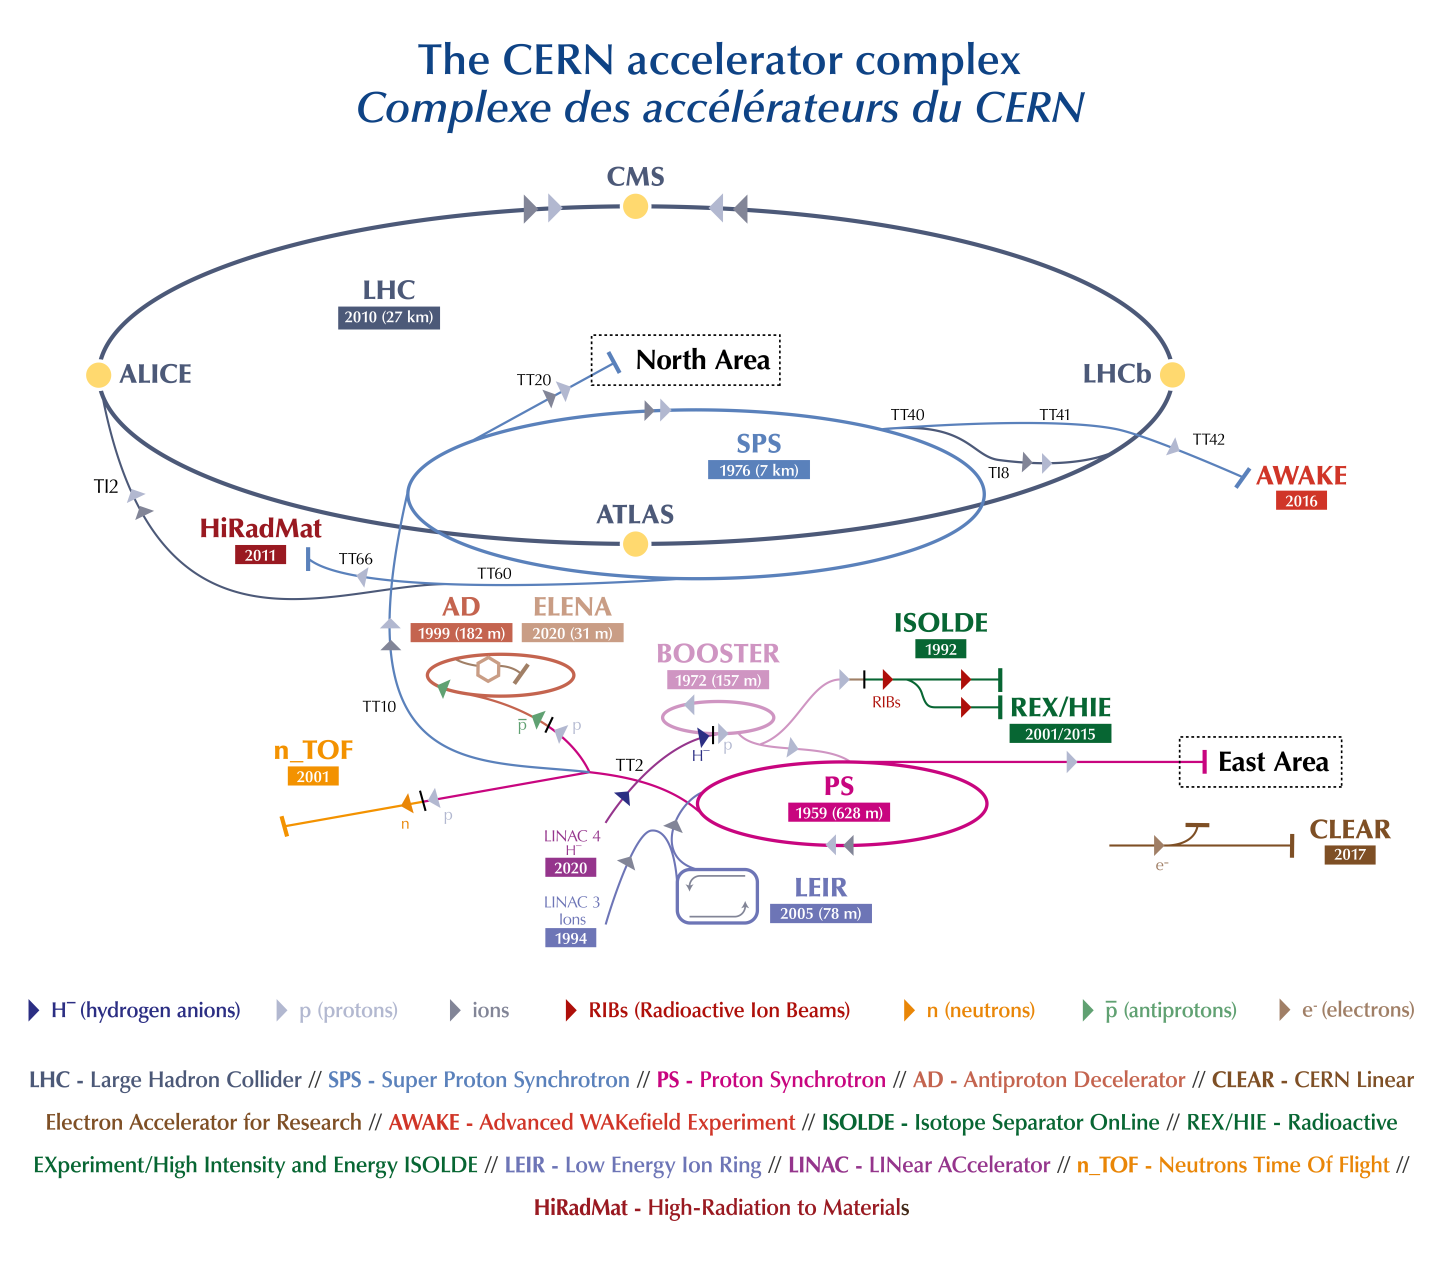
\includegraphics[width=\textwidth]{CCC-v2019-final-white_small}
    \caption{CERN has various accelerators and decelerators. H$^-$ ions are pre-accelerated
    in LINAC2 (LINAC4 in the future) and passed to PSBooster, PS, SPS and finally injected into
    the LHC. Image credit: \cite{CERN_AccCmplx}}
    \label{fig_cern_acc_cmplx}
\end{figure}
%
Heavy ions start in the LINAC3 and are then accelerated in the Low Energy Ion Ring (LEIR) before they are injected into
the PS from where they continue as described for protons.

The LHC consists of eight identical arcs for bending of the beams and eight straight sections between the
arcs which contain the experiments, injection and extraction region and accelerating structures.

An arc consists of 23 so called \emph{FODO}~cells containing two bending sections interleaved with
a focusing and a defocusing quadrupole\footnote{
    The acronym FBDB for focusing-bending-defocusing-bending would be more precise but this work will follow
    the common denomination.
}.
To correct for magnet imperfections, corrector magnets are also installed in the cell.
\figureref{fig_fodo} shows a schematic of an LHC FODO cell.
%
\begin{figure}[h]
    \centering
    \includestandalone[width=\linewidth]{fodo} 
    \caption{
        Schematic of an LHC FODO cell. Two bending sections, consisting of 3 bending dipoles each
        are interleaved by one focusing and one defocusing quadrupole, respectively.
    }
    \label{fig_fodo}
\end{figure}
%
During long shutdown 2, from 2019 until 2021, the CERN accelerator complex undergoes an extensive upgrade process 
preparing it already partly for the high luminosity upgrade of LHC.
In addition, the injector chain is upgraded in a separate project called \emph{LHC Injector Upgrade} (LIU) \cite{Hanke2017,Bartosik2017}.

% --------------------------------------------------------------------------------------------------
% Intro to OMC
% --------------------------------------------------------------------------------------------------
\section{Optics measurements and corrections}

There are two areas for which the continued measurement and correction of optics parameters is of
importance. The first is machine protection. If the nominal LHC beam hits the wall of the beam pipe
it can deal severe damage to the elements ranging from heating up superconducting elements and
inducing a magnet quench to physically destroying machine parts by melting (or even evaporating) the
material.

The second area for which  optics control is highly important is the machine performance.
The delivered luminosity can be reduced by optics errors.
The two main LHC experiments, ATLAS and CMS demand a luminosity imbalance below $\SI{5}{\percent}$.
To achieve this an optics correction up to the percent level is needed.
High quality optics also improve operational efficiency.

% --------------------------------------------------------------------------------------------------
% Measurement tools and techniques
% --------------------------------------------------------------------------------------------------
\subsection{Measurement tools and techniques}

The most important technique for beam based optics measurements that is applied in the LHC is the excitation
of the particle beam.
If the bunch is excited it performs a betatron oscillation about the closed orbit with a measurable amplitude.
The position of the beam is recorded at certain positions in the accelerator at each revolution. The
obtained turn-by-turn data is then analysed as described later.

To obtain said excitation there are two methods that will be introduced in this section: a free kick
which provokes a free oscillation of the bunch and an AC-dipoles which drives a forced oscillation of
the beam. 

% --------------------------------------------------------------------------------------------------
\subsubsection{Free Kick}

If the beam experiences a kick it will perform a damped free oscillation.
The particle's position at the same location turn after turn is illustrated in \figref{fig_kick_plot}.
Light particles like electrons
suffer from a strong damping because of their high synchroton radiation but heavier particles like the
protons accelerated in the LHC are damped much slower.
Nevertheless the oscillation amplitude decreases fast and not many turns are available for high
precision measurements of the turn-by-turn signal. In order to still have as much signal as possible
the kick strength has to be as high as feasible without kicking the beam strongly enough to damage elements or even kick it out of the accelerator.

Furthermore the excitation by a single kick carries the risk of filamenting the
phase space and blowing up the beam emittance.
%
\begin{figure}[h]
    \centering
    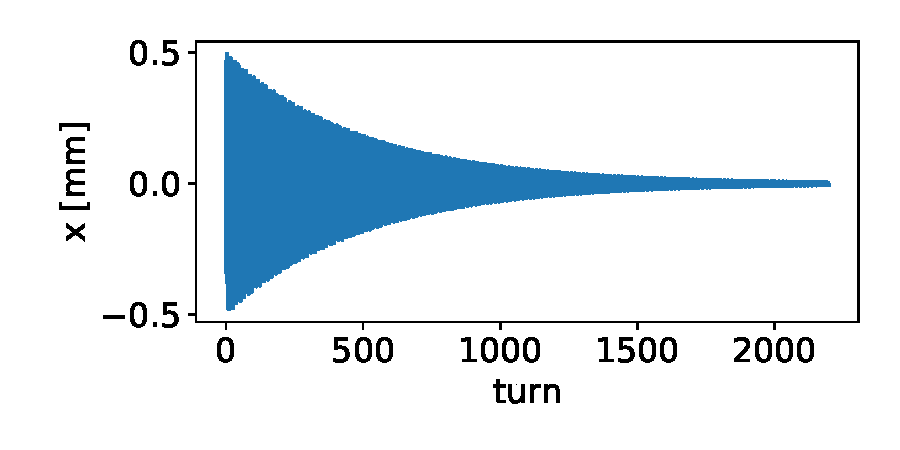
\includegraphics[width=.8\linewidth]{kick_plot.pdf}  
    \caption{The particle's turn-by-turn position for an excitation by a single kick.}
    \label{fig_kick_plot}
\end{figure}
%
\subsubsection{AC-dipole}

The other method to excite the beam that is used in LHC is a dipole connected to an alternate current
power amplifier.
This creates a driven oscillation of the beam \cite{Peggs1998} which can be measured in BPMs \cite{Miyamoto2008, Miyamoto2010}.
The excitation amplitude is slowly ramped up for 2000 turns in order to stay in an
adiabatic regime \cite{Tomas2005ac} held constant for 6600 turns and then again adiabatically ramped down.
The particle's turn-by-turn position is illustrated in \figref{fig_ac_plot}.

The adiabatic ramp up and down prevent a blow up of the beam emittance and since the oscillation amplitude
can be held constant, a smaller maximum amplitude is needed. 
%
\begin{figure}[h]
    \centering
     \begin{tikzpicture}
    \node (b1) {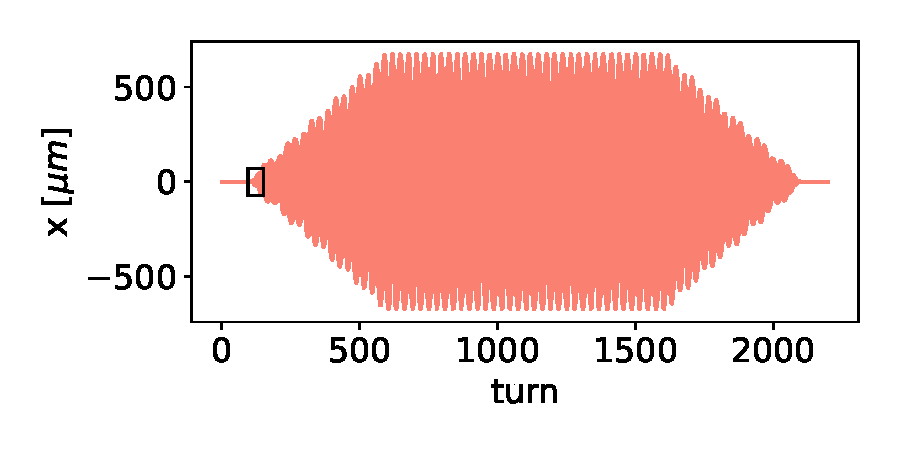
\includegraphics[width=.8\linewidth]{./ac_plot}};
    \node at ($(b1) + (3.2,2.2)$) {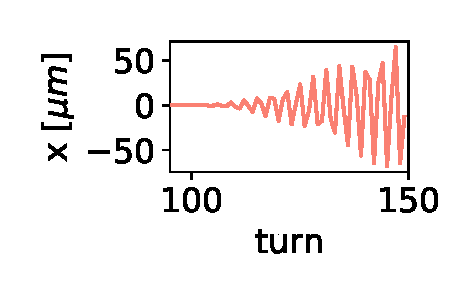
\includegraphics[width=.4\linewidth]{./ac_plot_zoom}};
    \end{tikzpicture}   
    \caption{
        The turn-by-turn position of an AC-dipole excitation. The driving force is ramped up,
        held at flat-top and ramped down again.
        The small plot shows a magnified view of the start of the ramp up.
    }
    \label{fig_ac_plot}
\end{figure}
%
Since the driven excitation creates a forced oscillation as opposed to a free one as in the case of
a single kick, the turn-by-turn motion of the particle does not reflect the pure betatron oscillation
and this effect has to be compensated. For this compensation a good theoretical knowledge of the driven
motion is needed.

%Another disadvantage of the AC-dipole in its current form in the LHC is a cooldown time of about
%one minute that can slow down the measurement process.

% --------------------------------------------------------------------------------------------------
\subsubsection{Beam Position Monitors}

To record the turn-by-turn position of the beam, the LHC possesses more than 500 dual-plane
Beam Position Monitors (BPMs) which are installed approximately regularly around the ring. 

The particle's transverse position in Complex Courant-Snyder coordinates at a location $s$ and turn
$N$ can be optained by applying repeatedly the one turn map:
%
\begin{equation}
    \hat{h}_z^\pm(s + NC) = \sqrt{2J_z} \e{i \left( \varphi_z(s) + 2\pi N Q_z\right)} 
    \fstop
\end{equation}
%
The real position and momentum of the particle can then be calculated by reversing the steps outlined
in the first section of this chapter.
%
\begin{equation}
    z(s + NC) = \sqrt{2J_z\beta_z(s)}\cos \left( \varphi_z(s) + 2\pi N Q_z\right)
\end{equation}
%
The phase $\varphi_z(s)$ and amplitude $\sqrt{2J_z\beta_z(s)}$ can be obtained by a Fourier transformation of
the particle positions.

\section{Outline of the thesis}

Chapter~\ref{ch_introduction} gives an introduction of the necessairy theory. Starting with linear beam 
dynamics it introduces the most important terminology before passing to the more mathematically involved
regime of normalised coordinates, adding up to the introduction of resonant driving terms which are used
to study beam optics throughout this work.
This formalism is then used to express the quantities needed in later chapters, in a useful form. 
Finally, the actual methods used to measure some machine parameters are described in detail giving the
reader an insight into where the newly developped methods will act.
No new discovery is presented in this chapter and it is a mere summary of the theoretical foundations.
Only subsection~\ref{sec_driven_coords} bears a minor amount of original work re-deriving the final form
of the forced coordinates in the used formalism, generalising it to an arbitrary position in the ring.



\chapter{Theoretical Foundations}
\label{ch_introduction}

\begin{chapterinfo}
    This chapter presents the basic theoretical foundations needed to develop
    the methods and algorithms presented in the main part of this thesis.
    Therefore we need a sound understanding of linear beam optics, 
    optics parameters like $\beta$~function and phase and, finally, linear transverse coupling.
    Only a brief summary of the vast field of accelerator physics can be given in the scope of this
    thesis. The interested reader may consult some of the great introductory works of the field, e.g.
    \cite{CAS2003, Wiedemann2015, WolskiBook}.

    Also the normal form approach shall be introduced here as it is needed to calculate optics
    parameters from Hamiltonian terms later on. Since this is a mathematically heavy subject,
    the author tried to find the optimum between brevity and rigor. 
    
    No new discoveries are presented in this chapter. It is a mere summary of the necessary theory.
    %No original work is presented in this chapter unless specified. The author did insert the
    %quadrupole example in sections~\ref{sec_beam_optics} and \ref{sec_hamil_lie} without consulting
    %any literature but these examples are so basic that the result is well known and the derivations
    %are for sure standard exercises in lectures on accelerator physics.

\end{chapterinfo}

%\section{A word on notation}
%Accelerator physics is a field, for sure not the only one, with notoriously bad notation and conventions.
%In multiple cases the same symbol is used to describe two or more completely different quantities.
%Keeping the notation of a work like this PhD thesis consistent is not an easy task on its own. Less so
%in the given situation.
%Therefore this little prolog serves in guiding the reader through the notations and conventions adopted
%throughout this thesis.
%\textbf{Planes} We describe the motion of the particles and beams in the regime of \emph{transverse beam dynamics} with
%two transverse planes $x$ and $y$.
%So we have to distinguish optical functions and variables by plane: $x, y, \beta_x, \alpha_x, \phi_x$.
%Most of the time however it is of no importance in which plane the equations
%are expressed or we work for an extended period in the same plane.
%In those cases, the index denoting the plane will be dropped. 
%\textbf{Vectors} are denoted by an italic letter with an arrow above. Phase space \textbf{coordinates} are
%usually denoted by lowercase latin letters ($\vec{x}, \vec{v}, \vec{p}$) with the exception of normal form coordinates
%which are greek lowarcase letters ($\vec{\zeta}, \vec{\xi}$). \textbf{Fields} are denoted by capital
%latin letters ($\vec{E}, \vec{B}$).
%\textbf{Matrices} are denoted by bold face letters, usually capital latin $\mat{M}, \mat{V}$.




%The Large Hadron Collider is the world's largest particle accelerator with the highest center of mass
%energy per charge unit. It has a circumference of $\SI{27}{km}$ and is situated at the French-Swiss 
%border near Geneva. The top energy for protons is $\SI{7}{TeV}$
%and in the lead ion run of 2018 a beam energy of $\SI{6.37}{Z TeV}$ was achieved.
%The particles pass through various pre-accelerators where they are accelerated in steps before being
%injected in the LHC at $\SI{450}{GeV}$. The complete accelerator complex at CERN is sketched in
%\figref{fig_cern_acc_cmplx}.

% --------------------------------------------------------------------------------------------------
% beam optics
% --------------------------------------------------------------------------------------------------
\section{Beam Optics}
\label{sec_beam_optics}

Very much like light beams, charged particle beams in an accelerator can be bent\footnote{%
the \emph{bending} of light is, of course, technically difficult to achieve}, focused, defocused
and can be subject to effects like dispersion and chromaticity. Therefore the term \emph{optics} is
generally used to describe the movement and behaviour of particle beams around the accelerator.

This work focuses on single particle dynamics, effects between the particles of a beam will be
neglected. 

\subsection{Linear Beam Dynamics}

Linear beam dynamics studies the effect of linear electromagnetic fields on the particles.
This includes primarily only drift spaces, bending magnets and (de)focusing magnets. Under the presence
of electromagnetic fields $\vec{E}$ and $\vec{B}$, the Lorentz force acts on the particles with charge
$q$ and velocity $\vec{v}$.
%
\begin{equation}
    \vec{F} = q\left(\vec{E} + \vec{v} \times \vec{B}\right)
    \fstop
    \label{eq_lorentz_force}
\end{equation}
%
A dipole with a constant magnetic field $B_y$ bends a particle's trajectory into an arc of radius $\rho$
%
\begin{equation}
    \rho = \frac{p}{qB_y}
    \fstop
    \label{eq_acc_radius}
\end{equation}
%
It is useful to describe the motion in a circular accelerator in a co-moving reference frame as
depictet in \figref{fig_frenet_serret}\index{Frenet-Serret coordinates} where the cartesian coordinates $\{x', y', z'\}$ are
transformed into a system $\{x,y,s\}$ with the properties:
%
\begin{align}
    \Delta s &\parallel \text{reference orbit}\notag\\
    \hat{y} &= \hat{y}'\notag\\
    \hat{x} &= \hat{y} \times \Delta s
\end{align}
%
and a longitudinal coordinate $s$ along the reference orbit.
\begin{figure}[ht]
    \includestandalone{frenetserret}
    \caption{
        The Frenet-Serret coordinate system which is moving along the design orbit of particles
        in the accelerator.
    }
    \label{fig_frenet_serret}
\end{figure}
%
The optical axis of the elements is usually used as reference orbit.
If there is no transverse offset of the elements, this coincides with the closed orbit.

In this coordinate system the motion of a particle in a circular accelerator is described by Hill's
differential equation\index{Hill's equation}:
%
\begin{equation}
    \frac{\der^2 z}{\der s^2} + k(s)z = 0
    %\fstop
    \label{eq_hills}
\end{equation}
%
where $z \in \{x,y\}$ is the transverse coordinate and $k(s)$ is the linear magnet strength at
position $s$.

A solution that satisfies \eqref{eq_hills} in two dimensions is
%
\begin{equation}
    z(s) = A_z(s) \cos\left(\phi_z(s) + \phi_{z,0} \right)
    \label{eq_betatron_osc}
\end{equation}
%
where the $s$-dependent amplitude of the oscillation can be split:
%
\begin{equation}
    A_z(s) = \sqrt{2J_z \beta_z(s)}
    \fstop
    \label{eq_betatron_ampl}
\end{equation}
%
$\beta_z(s)$ is the $s$-dependent part of the amplitude, called $\beta$~function\index{$\beta$ function}.
$J_z$ is the action invariant of the particle's motion.
$\beta(s)$ is periodic with the circumference of the ring $C$.

Of special interest for a collider is the value of the $\beta$~function at the interaction point,
 because it defines the beam size and
has a high impact on the luminosity, as follows from \eqref{eq_lumi}.
At the LHC, the $\beta$~function at the interaction point is denoted as $\beta^* \equiv \beta(s_\text{IP})$
whereas the \emph{smallest} $\beta$~function is called $\beta_\text{waist}$.

$\phi(s)$ is called the \emph{betatron phase} and satisfies the following property:
%
\begin{equation}
    \phi(s_1) - \phi(s_0) = \int\limits_{s_0}^{s_1} \frac{1}{\beta(s)}\der s
    \fstop
    \label{eq_phase}
\end{equation}
%
The trajectories of particles with an action $J$ are limited by an envelope function $\sqrt{2J\beta}$ as illustrated in Fig.~\ref{fig_part_traj}.
%
\begin{figure}[ht]
    \centering
    %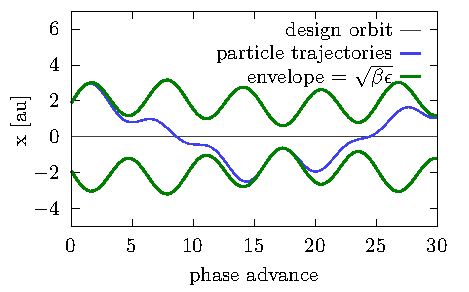
\includegraphics[width=.49\linewidth]{particle_traj_beta_1}
    %\hfill
    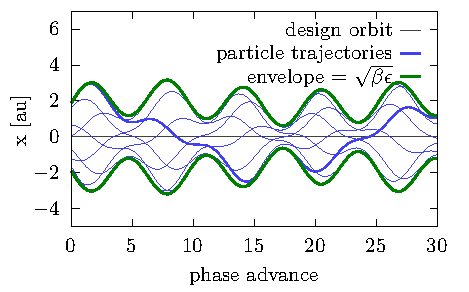
\includegraphics[width=.7\linewidth]{particle_traj_beta_many_wb}
    \caption{The trajectories of particles with action $J$ are shown.}
    \label{fig_part_traj}
\end{figure}
%
Actual $\beta$~functions are shown in Fig.~\ref{fig_beta}.
%
\begin{figure}[ht]
  \centering
  \footnotesize
  \includestandalone[width=\linewidth]{./twiss/IP_beta_x}
  \includestandalone[width=\linewidth]{./twiss/Arc_beta_x}
  \normalsize
  \caption{
    TOP: The $\beta$~function around IP1.
    BOTTOM: The $\beta$~functions in an LHC arc, the plot ranges from IR2 to IR3,
    avoiding high~$\beta$ regions (IR1 and IR5) shown in the top plot.
    Both plots show the LHC collision optics at $\beta^*=\SI{30}{cm}$.
  }
  \label{fig_beta}
\end{figure}

Solutions of \eqref{eq_hills} can be expressed in matrix form
%
\begin{equation}
    \begin{pmatrix}
        z\\
        p_z
    \end{pmatrix}_b
    =
    \begin{pmatrix}
        m_{11} & m_{12} \\
        m_{21} & m_{22}
    \end{pmatrix}
    \begin{pmatrix}
        z\\
        p_z
    \end{pmatrix}_a
    \fstop
    \label{eq_matrix_element}
\end{equation}
%
Throughout this work, the following definition of momentum is used:
\begin{equation}
  p_z \equiv \frac{\der z}{\der s}
  \fstop
\end{equation}
The reference frame spanned by $z$, $p_z$ is called \emph{phase space}%
\footnote{%
Sometimes the name phase space is reserved for the reference frame spanned by $\left(z,\frac{\der z}{\der t}\right)$ %
whereas the one spanned by $\left(z,\frac{\der z}{\der s}\right)$ is called \emph{trace space}. %
This work will, however, follow the convention stated in the main text.%
}%
.

The matrix 
%
\begin{equation}
    \mat{M} = 
    \begin{pmatrix}
        m_{11} & m_{12} \\
        m_{21} & m_{22}
    \end{pmatrix}
    \label{eq_trmat}
\end{equation}
%
is called the \emph{transfer matrix}\index{transfer matrix}. It describes the transformation
of phase space when going from one position $s_a$ in the lattice to another $s_b$.

At this point in an introductory text of, e.g. a thesis or a textbook on accelerator physics
it is customary to give a simple example, a basic linear lattice element like a drift space or
a quadrupole for illustration.
The author chooses to present a quadrupole magnet, since the effect of quadrupolar imperfections
is dealt with in later chapters. This example is revisited in the more complex frameworks of
Hamiltonian mechanics and Lie maps to guide the reader.

For $s$ inside the quadrupole $k(s) = k_1$ . The solution of Hill's equation is
%
\begin{equation}
    z(s) = \cos \left[ \sqrt{k}(s-s_0)\right] z_0 +
        \frac{1}{\sqrt{k}}\sin\left[\sqrt{k}(s-s_0)\right]p_{z,0}
    \label{eq_quad_transfer}
    \fstop
\end{equation}
%
The transfer matrix of a focusing quadrupole reads
%
\begin{equation}
    \mat{M}_{QF} =
    \begin{pmatrix}
        \cos \sqrt{K} & \frac{1}{\sqrt{k}} \sin \sqrt{K} \\
        -\sqrt{K}\sin \sqrt{K} & \cos \sqrt{K}
    \end{pmatrix}
    \label{eq_trmat_quad}
\end{equation}
%
where $K$ is the integrated magnet strength
%
\begin{equation}
    \sqrt{K} = \int\limits_{s_i}^{s_i + L} \sqrt{k(s)}\der s
\end{equation}
%
for a quadrupole at position $s_i$ with length $L$.

A purely linear accelerator can than be constructed by the composition of the transfer matrices of 
all its elements. This composition yields a special example of the transfer matrix, the one that
transforms the phase space coordinates of a particle at a given position to the same position in the
next turn\index{one turn map}:
%
\begin{equation}
    \mat{M}_\text{OT} = \prod\limits_{w=1}^W \mat{M}_i
\end{equation}
%
where $\mat{M}_w$ is the transfer matrix of the $w$th element, $W$ is the number of elements in the
accelerator and the product denotes the repeated matrix multiplication from the left.
\begin{figure}
    \centering
    \includestandalone[width=0.7\linewidth]{fig_lattice}
    \caption{This schematic represents the accelerator lattice, consisting of consecutive maps
    $\mathbf{M}_1 \ldots \mathbf{M}_W$.
    }
    \label{fig_lattice}
\end{figure}
%
Figure~\ref{fig_lattice} illustrates this setup.
The phase advance of one turn
%
\begin{equation}
    Q_z \equiv \frac{1}{2\pi}\int\limits_{s_0}^{s_0+C} \frac{\der s}{\beta_z(s)}
    \komma
\end{equation}
%
normalised by $2\pi$, is called the \emph{betatron tune}\index{tune}\index{betatron tune}.

A general form of \eqref{eq_trmat} is 
%
\begin{equation}
    \begin{pmatrix}
        \sqrt{\frac{\beta_b}{\beta_a}}(\cos\phi_{ab} + \alpha_a \sin\phi_{ab}) &
        \sqrt{\beta_a\beta_b} \sin\phi_{ab} \\
        \frac{\alpha_a - \alpha_b}{\sqrt{\beta_a\beta_b}}\cos\phi_{ab} - \frac{\beta+\alpha_a\alpha_b}{\sqrt{\beta_a\beta_b}}\sin\phi_{ab} &
        \sqrt{\frac{\beta_a}{\beta_b}}(\cos\phi_{ab} - \alpha_b\sin\phi_{ab})
    \end{pmatrix}
    \label{eq_trmat_01}
\end{equation}
%
where the quantity
%
\begin{equation}
    \alpha(s) = -\frac{1}{2}\frac{\der \beta(s)}{ \der s}
    \label{eq_alpha}
\end{equation}
%
is called $\alpha$~\emph{function}\index{$\alpha$ function}.
%
$\alpha$, $\beta$ function and a third quantity
%
\begin{equation}
    \gamma(s) = \frac{1+\alpha^2(s)}{\beta(s)}
\end{equation}
%
are called \emph{Twiss~parameters}.

For convenience and later usage we introduce the following short-hand notation:
%
\begin{equation}
    \phi_{z,ab} = \phi_z(s_b) - \phi_z(s_a) + 2\pi Q_z \Theta(s_a, s_b)
\end{equation}
%
which is the \emph{phase advance}\index{phase advance} between position $s_a$ and $s_b$, taking into
account the relative position of $s_a$ to $s_b$.
If element $b$ lies upstream from element $a$, the interval \emph{wraps around} the end of the
lattice definition and the tune
has to be added to the phase advance. For this the following definition is used:
%
\begin{equation}
    \Theta(s_a, s_b) =
    \begin{cases}
        1 & \text{if } s_a > s_b \\
        0 & \text{else} \\
    \end{cases}
    \fstop
\end{equation}
%
The particles motion in phase space follows a tilted ellipse which is described by
%
\begin{equation}
    \gamma(s)z^2(s) + 2\alpha(s)z(s)p_z(s) + \beta(s)p_z^2(s) = 2 J_z
\end{equation}
%
where $J_z$ is called the \emph{action}%
\footnote{
    Often a quantity $\epsilon^\text{part}_z=2 J_z$ is defined, called the single particle emittance.
    It must not be confused with the \emph{beam emittance}
    $\epsilon_z = \frac{1}{2}\langle \epsilon_z^\text{part} \rangle$.
}%
. The area of the ellipse is $2J_z\pi$.

The one turn map in this form can be retrieved by setting $\beta_a = \beta_b $, ${\alpha_a = \alpha_b}$
and ${\phi_{ab} = 2\pi Q}$:
%
\begin{equation}
    M_\text{OT} = \begin{pmatrix}
        \cos(2\pi Q_z) + \alpha_a \sin(2\pi Q_z) & \beta_a\sin(2\pi Q_z) \\
        -\gamma\sin(2\pi Q_z) & \cos(2\pi Q_z) - \alpha_a\sin(2\pi Q_z)
    \end{pmatrix}
    \fstop
\end{equation}
%

% --------------------------------------------------------------------------------------------------
% --- Courant Snyder Coordinates
% --------------------------------------------------------------------------------------------------
\subsection{Courant-Snyder coordinates}
\label{sec_intro_cs}
If one plots the phase space of a particle at a certain position $s_a$ over many turns, it draws an
ellipse with area $2J_z\pi$ where $J_z$ is called \emph{action}.
Particle motion is easier expressed in Courant-Snyder coordinates \cite{Courant1958, Bazzani1994}
%
\begin{equation}
    \begin{pmatrix}
        \hat{z}\\
        \hat{p_z}
    \end{pmatrix}
    =
    \begin{pmatrix}
        \frac{1}{\sqrt{\beta_z}} & 0\\
        \frac{\alpha_z}{\sqrt{\beta_z}} & \sqrt{\beta_z}
    \end{pmatrix}
    \begin{pmatrix}
        z\\
        p_z
    \end{pmatrix}
    \label{eq_cs_matrix}
\end{equation}
%
\begin{figure}[ht]
    \centering
    \includestandalone{figures/xp_linear}
    \hspace{1cm}
    \includestandalone{figures/cs_linear}
    \caption{In physical coordinates the turn-by-turn movement of the particle draws an ellipse.
        Transformation to Courant-Snyder
        coordinates turns this ellipse into a circle.}
    \label{fig_phase_space_ellipse}
\end{figure}
%
which transforms the phase space ellipse into a circle with radius $\sqrt{2J_z}$.
The transformation is illustrated in Figure~\ref{fig_phase_space_ellipse_nl}.
In the following Courant-Snyder coordinates will frequently be abreviated by \emph{CS coordinates}.

The transformation matrix in \eqref{eq_cs_matrix} is called $\mat{T}$ for the rest of this chapter.
Applying $\mat{T}$ to the one turn map, one can see that the one-turn evolution of the particle is
now a rotation of $2\pi Q_z$:
\begin{equation}
    \mat{T}\;\mat{M}_\text{OT}\;\mat{T}^{-1} = 
    \begin{pmatrix}
        \cos(2\pi Q_z) & -\sin(2\pi Q_z)\\
        \sin(2\pi Q_z) & \cos(2\pi Q_z) \\
    \end{pmatrix}
    \fstop
\end{equation}

It is often convenient to express the Courant-Snyder coordinates in their complex form:
%
\begin{equation}
    h^\pm_z \equiv \hat{z} \mp i \hat{p}_z
    \label{eq_courantsnyder}
\end{equation}
%
and the one turn map simplifies further to a rotation about $2\pi Q_z$, 
%%
%\begin{equation}
%    \mat{M}_\text{OT} \varphi_z = \varphi_z + 2\pi Q_z
%    \fstop
%\end{equation}
%%
%The action on the complex Courant-Snyder coordinates reads
%
\begin{equation}
  \mat{M}_{\text{OT}} h_z^\pm = \e{\mp 2\pi i Q_z}h_z^\pm
  \fstop
\end{equation}

In a linear lattice, the particle motion in complex Courant-Snyder coordinates at turn $N+1$ and position
$s$ in the ring reads
%
\begin{equation}
    h_z^\pm(s,N) = \sqrt{2J_z} \e{\mp i \left[2N\pi Q_z + \varphi_z(s) + \varphi_{z,0}\right]}
\end{equation}
%
with $\varphi_{z,0}$ being a phase offset given by initial conditions.

The formulae above assume no coupling between the transverse planes.
Before we continue to dive into the depths of general normalised coordinates for non-linear
optics, we introduce more general coordinates and maps, mixing the two planes:
\begin{equation}
    \begin{pmatrix}
        x \\ p_x \\ y \\ p_y
    \end{pmatrix}_b
    =
    \mat{M}\;
    \begin{pmatrix}
        x \\ p_x \\ y \\ p_y
    \end{pmatrix}_a
\end{equation}
where the transfer map $\mat{M}$ now is a $4\times 4$ matrix.
For convenience, the vector containing the 4D coordinates will be called $\vec{z}$.

% --------------------------------------------------------------------------------------------------
% Lie maps and hamiltonian
% --------------------------------------------------------------------------------------------------
\section{Hamiltonian description and Lie maps}
\label{sec_hamil_lie}

Some preliminaries are needed to describe the particle motion using the Hamiltonian description
and Lie transformations.
A thorough repetition of the topic of Lie groups and Lie algebras can not be given in the
scope of this thesis, the reader may consult \cite{Georgi1982}.

The general Hamiltonian of a charged particle in a circular accelerator is \cite{WolskiBook, Herr2020}
%
\begin{equation}
    %H=-\left( 1+\frac{x}{\rho} \right) \sqrt{(1+\delta)^2 -p_x^2-p_y^2}
    %+ \frac{x}{\rho} + \frac{x^2}{2\rho^2} - \frac{A_s(x,y)}{B_0\rho}
    \hat{H}=\frac{\delta}{\beta_0} - (1+hx)
    \sqrt{
      \left(\delta + \frac{1}{\beta_0} - \frac{q\phi}{cP_0}\right)^2 - (p_x-a_x)^2 - (p_y-a_y)^2
      - \frac{1}{\beta_0^2\gamma_0^2}
    }
    - (1+hx)a_s
\end{equation}
with the following definitions:

\begin{tabular}{ll}
  $P_0$ & reference momentum, \\
  $\delta = \frac{p_z}{P_0}$ & relative longitudinal momentum deviation, \\
  $h=\frac{1}{\rho}$ & local curvature with $\rho$ being the local curvature radius, \\
  $\beta_0$, $\gamma_0$ & relativistic factors, \\
  $q$ & the particle's charge, \\
  $\phi$ & the electric field, \\
  $a_x = \frac{q}{P_0}A_x, a_y = \frac{q}{P_0}A_y$ & the normalised transverse components of the vector potential $(A_x, A_y)$, \\
  $a_s = \frac{q}{P_0}A_s$ & the normalised longitudinal component of the vector potential
\end{tabular}

The Hamiltonian equations of motion \cite{Landau1976} read
\begin{align}
    \frac{\der z}{\der s}=\frac{\partial \hat{H}}{\partial p_z} \quad\text{ and }\quad
    \frac{\der p_z}{\der s}=-\frac{\partial \hat{H}}{\partial z}
\end{align}
%
for canonical variables $z$ and $p_z$.
The previous example of a quadrupole is again used to demonstrate this approach.
The Hamiltonian for a particle moving through a single quadrupole is obtained from putting the
corresponding vector potential
%
\begin{align}
  a_s &= -\frac{k_1}{2}(x^2 - y^2) \\
  a_x &= a_y = \phi = 0
\end{align}
%
and 0 curvature ($h = 0$):
%
\begin{align}
    \hat{H} &=\frac{\delta}{\beta_0}
      - \sqrt{\left(\delta + \frac{1}{\beta_0}\right)^2 - p_x^2 - p_y^2 - \frac{1}{\beta_0^2\gamma_0^2}}
      + \frac{k_1}{2}(x^2 - y^2) \\
    \hat{H} &= \frac{p_x^2 + p_y^2}{2} + \left(\frac{\delta}{2\beta_0\gamma_0}\right)^2
    + \frac{k_1}{2}(x^2 - y^2)
    + O(2nd)
    \fstop
    \label{eq_hamil_quad_delta}
\end{align}
%
In the simple example at hand, only one on-momentum particle is considered:
%
\begin{equation}
    \hat{H} = \frac{k_1}{2}\left( x^2 - y^2 \right) + \frac{p_x^2+p_y^2}{2}
    \label{eq_hamil_quad}
\end{equation}
%
Plugging this consecutively into the Hamiltonian equations of motion, yields
\begin{align}
    \frac{\der x}{\der s} &= \frac{\partial \hat{H}}{\partial p_x} = p_x \\
    \Rightarrow \frac{\der^2 x}{\der s^2} &= \frac{\der p_x}{\der s} = -k_1x
\end{align}
which coincides with Hill's equation, \eqref{eq_hills}.

Poisson brackets,
%
\begin{equation}
    [f,g] = 
    \sum\limits_{z\in\{x,y\}}
    \left(
    \frac{\partial f}{\partial z} \frac{\partial g}{\partial p_z}
    - \frac{\partial f}{\partial p_z}\frac{\partial g}{\partial z}
    \right)
    \komma
\end{equation}
%
can be used to rewrite the Hamiltonian equations:
\begin{align}
    [z, \hat{H}] = \frac{\partial \hat{H}}{\partial p_z}\quad\text{ and }\quad
    [p_z, \hat{H}] = -\frac{\partial \hat{H}}{\partial z}
    \fstop
\end{align}
%
The Poisson brackets form a \emph{Lie algebra} and therefore some properties can be utilised.
First, we define a \emph{Lie operator} acting on $g$
\begin{equation}
    \liemap{f}g = [f,g]
    \fstop
\end{equation}
Then we can use the exponential parameterisation of Lie groups to move away from the origin
\cite{Georgi1982} and describe the particle motion going through an element $w$ in the lattice
using the \emph{kick Hamiltonian} of this element,
which is constructed by multiplying the thin lens Hamiltonian by the length of the element,
$H=\hat{H}L$%
%
\begin{equation}
    x(s_b) = \e{\liemap{H}}x(s_a)
    \label{eq_exponential_map}
    \komma
\end{equation}
with $L$ being the length of the element.
%
To illustrate this, once again the quadrupole is used. Some helpful identities, for convenience:
\begin{align}
    \liemapn{g}{2} &= \liemap{g}\circ\liemap{g}\notag \\
    \liemap{x^2} f(x,p_x) &= 2x\frac{\partial f(x,p_x)}{\partial p_x} \notag \\
    \liemap{p^2} f(x,p_x) &= -2p_x\frac{\partial f(x,p_x)}{\partial x}
   % \notag \\
   % \liemapn{x}{n} f(x,p_x) &= \frac{\partial^n f(x,p_x)}{\partial p_x^n} \notag \\
   % \liemapn{p}{n} f(x,p_x) &= -\frac{\partial^n f(x,p_x)}{\partial x^n}
   \fstop
\end{align}
%
Now it is possible to show
\begin{align}
    x(s_b) = \e{\liemap{H}} x(s_a) &= x(s_a) - Lp_x(s_a)
        - \frac{1}{2}L^2k_1x(s_a) + \frac{1}{6}L^3k_1p_x(s_a)
        \notag \\
        &\quad + \frac{1}{24}k_1^2x(s_a) - \frac{1}{120}k_1^2p_x(s_a)
        + \ldots
        \notag \\
       &= x(s_a) \cos(L\sqrt{k_1}) - \frac{p(s_a)}{L\sqrt{k_1}} \sin(L\sqrt{k_1})
\end{align}
which agrees with the propagation through a quadrupole given in \eqref{eq_quad_transfer},
noting that the Hamiltonian, and therefore $k$, is constant inside the (ideal) quadrupole described by the
Hamiltonian~\eqref{eq_hamil_quad}.
Usually, non-linear terms are collected into a non-linear map $\e{\liemap{H}}$, generated
by the non-linear Hamiltonian and a linear transfer map (rotation in CS-coordinates) $\mat{M}$:
%
\begin{equation}
    \mathscr{M}_w = \e{\liemap{H_w}} \mat{M}_w
    \komma
\end{equation}
%
where the subscript $w$ denotes the map of element $w$ in the lattice and the particle motion
is propagated through the element by
\begin{equation}
    \vec{z}(s_w + L) = \e{\liemap{H_w}} \mat{M}_w \vec{z}(s_w)
\end{equation}
for element $w$ with length $L$.
 


% --------------------------------------------------------------------------------------------------
% Normal forms and RDTs
% --------------------------------------------------------------------------------------------------
\section{The normal form approach}
\label{sec_normal_form}

In order to derive optics parameters from Hamiltonian terms the normal form approach\index{normal form}
-- usually encountered in treatments of non-linear optics -- is useful.
It is described in its full mathematical detail in \cite{Bartolini1997,Bazzani1994}
and more illustrative in \cite{Tomas2005, Herr2013, Herr2020}.

In the formalism of complex CS-coordinates, a transfer map can be written as
%
\begin{equation}
    \begin{pmatrix}
        h_x^+ \\ h_x^- \\ h_y^+ \\ h_y^-
    \end{pmatrix}_b
    =
    \mat{M}\;
    \begin{pmatrix}
        h_x^+ \\ h_x^- \\ h_y^+ \\ h_y^-
    \end{pmatrix}_a
    %\fstop
\end{equation}
%
where
%
\begin{equation}
 \mat{M}  = \
 \begin{pmatrix}
   m_{1000}^1 & m_{0100}^1 & m_{0010}^1 & m_{0001}^1 \\
   m_{1000}^2 & m_{0100}^2 & m_{0010}^2 & m_{0001}^2 \\
   m_{1000}^3 & m_{0100}^3 & m_{0010}^3 & m_{0001}^3 \\
   m_{1000}^4 & m_{0100}^4 & m_{0010}^4 & m_{0001}^4 \\
 \end{pmatrix}
 \fstop
\end{equation}
The significance of the multi-index $m_{jklm}^i$ will become clear in a moment.
It shall be noted that some symmetry relation applies:
%
\begin{equation}
  m_{jklm} = \conj{m_{kjml}}
\end{equation}
%

The map of a non-linear lattice element $i$ cannot be described by a matrix $\mat{M}_i$ only.
A higher order map is necessary. Here the multi-index comes into play.
Higher order maps $\mathcal{M}$ are composed of higher order polynomials:
%
\begin{equation}
    h_x^+(s_b) = \sum\limits_{n=1}^\infty\sum\limits_{j+k+l+m=n} m^1_{jklm}
        \left( h_x^+(s_a) \right)^j
        \left( h_x^-(s_a) \right)^k
        \left( h_y^+(s_a) \right)^l
        \left( h_y^-(s_a) \right)^m
    \fstop
\end{equation}
%

The transformation to Courant-Snyder coordinates flattens the phase space of linear optics to a circle.
For non-linear optics where the phase space motion is far more complicated the normal form approach
can be used to transform to a new set of coordinates, the \emph{normal form coordinates}
(their exact form will be defined at the end of this section), in which the
the phase space motion is flattened to a circle.
Figure~\ref{fig_phase_space_ellipse_nl} illustrates how particle trajectories inside a non-linear
machine evolve in phase space, CS-space and normal form space.
The irregular shape of in phase space is tilted to a more "upright" form in CS-space but only a
transformation to normal form space flattens the trajectory to a circle.

\begin{figure}[ht]
    \centering
    \includestandalone{figures/xp_nonlinear}
    \includestandalone{figures/cs_nonlinear}
    \includestandalone{figures/nf_nonlinear}
    \caption{
      If non-linearities are present in the lattice, the phase space motion of the particles is
      deformed and does not show the form of an ellipse any more. 
      Transformation to Courant-Snyder
      coordinates tilts the phase space but does not remove irregular deformations.
      Only a transformation into normal form coordinates restores a perfect circle.
    }
    \label{fig_phase_space_ellipse_nl}
\end{figure}

This map is generated by the non-linear Hamiltonian of the element.
The Hamiltonian of element $w$ evaluated at position $s$ in multipolar expansion,
reads
\begin{equation}
  H_w =
  -\re{\sum\limits_{n\ge 2} (K_{n-1} + i J_{n-1}\frac{(x+iy)^n}{n!})}_w
  \label{eq_gen_hamil}
\end{equation}
%
where $K_{n-1}$ and $J_{n-1}$ are normal and skew integrated multipolar field strengths,
%
\begin{align}
  K_n &= \frac{1}{n!}\frac{\partial^n B_y}{\partial x^{n}}\\
  J_n &= \frac{1}{n!}\frac{\partial^n B_x}{\partial x^{n}}
\end{align}
%
i.e. a pure dipole has only $K_0$, a pure quadrupole only $K_1$ etc.

In complex Courant-Snyder coordinates, the Hamiltonian~\eqref{eq_gen_hamil}, evaluated at position $s_i$,
can be written in the form
%
\begin{equation}
    H_w(s_i) = \sum\limits_{n\geq2} \sum\limits_{j+k+l+m=n} h_{w,jklm}
    \e{i \left[
        (j-k) \varphi_{x,wi} + (l-m) \varphi_{y,wi}
    \right]}
    \left(h_x^+\right)^j
    \left(h_x^-\right)^k
    \left(h_y^+\right)^l
    \left(h_y^-\right)^m
    \komma
\end{equation}
%
where the Hamiltonian term $h_{w,jklm}$ is defined as
%
\begin{equation}
    h_{w,jklm} = 
    \frac{
        \Omega(l+m) K_{w,n-1} + i\left[1-\Omega(l+m)\right] J_{w,n-1}
    }{
        j!\,k!\,l!\,m!\,2^{j+k+l+m}
    }
    i^{l+m}
    (\beta_{x,w})^{\frac{j+k}{2}}
    (\beta_{y,w})^{\frac{l+m}{2}}
    \fstop
    \label{eq_hamiltonianterm}
\end{equation}
%
The Hamiltonian of the whole lattice is denoted by
%
\begin{equation}
    H(s_i) = \sum\limits_w^W H_w(s_i)
    \label{eq_Hamil_sa}
    \fstop
\end{equation}
%
In \eqref{eq_hamiltonianterm} $\beta_{z,w}$ is the $\beta$ function of the corresponding plane at position $w$
and
%
\begin{equation}
    \Omega(a) = 
    \begin{cases}
        1 &\text{ if a is even} \\
        0 &\text{ if a is odd} \\
    \end{cases}
    \fstop
\end{equation}
%
The one-turn map of an accelerator now reads
%
\begin{equation}
    \mathscr{M}_\text{OT} = \prod\limits_{i=0}^W \e{\liemap{H_i}} \mat{M}_i
    \label{eq_one_turn_lie}
    \fstop
\end{equation}
%
It shall be noted that Lie maps do not, in general, commute and, in order to construct
a one-turn equivalent of the Hamiltonian, the Baker-Campbell-Hausdorff formula has to be applied:
%
\begin{equation}
    \e{\liemap{H_1}}\e{\liemap{H_2}} = \e{\liemap{H_1 + H_2 + \frac{1}{2}[H_1,H_2]
    + \frac{1}{12} [H_1, [H_1, H_2]] + \ldots}}
    \komma
\end{equation}
%
as opposed to~\eqref{eq_Hamil_sa} which is only a simple summation of Hamiltonian coefficients
to build one single Hamiltonian operator.

The transformation from complex Courant-Snyder coordinates to normal form coordinates and back is performed
using a generating function $F$:
%
\begin{align}
    \zeta_z^\pm &= \e{-\liemap{F}} h_z^\pm 
    \label{eq_z_from_h} \\
    h^\pm &= \e{\liemap{F}} \zeta_z^\pm
    \label{eq_h_from_z}
    \fstop
\end{align}
%
The \emph{normal form coordinates}\index{normal form!coordinates} $\zeta_z^\pm$
can be expressed in terms of the normal form phase $\psi$ and normal form invariant $I_z$:
%
\begin{equation}
    \zeta_z^\pm(s_i) = \sqrt{2I_z}\e{i\left[\mp \psi_z(s_i) + \psi_{z,0} \right]}
    \fstop
\end{equation}
%
Since $\psi$ and $I_z$ are canonical variables, the Poisson bracket between any of the normal form
coordinates can be calculated easily:
%
\begin{equation}
    \left[ \zxpto{n}, \zxmto{m}\right] = -2i\,nm\zxpto{n-1}\zxmto{m-1}
    \komma
    \label{eq_poiss_br_ident}
\end{equation}
and all other combinations are zero.
%

\section{Resonance driving terms}
\label{sec_rdts}

The following commutative diagram shows the transformation from the Courant-Snyder one turn map to 
the normal form one turn map:

\newcommand{\nfMotion}{\mathbfscr{M}_\text{OT}}
\newcommand{\nfOrtho}[1]{#1^\ddagger}
%
\begin{equation}
    \centering
        \begin{tikzcd} [row sep=large,column sep=8em]
            \vec{\zeta}(N) \arrow[r, "\nfMotion=\e{\liemap{\phiave{H}}}R"]
                & \vec{\zeta}(N+1) \\
            \vec{h}(N) \arrow[r, "\mathscr{M}_\text{OT}"'] \arrow[u, "\e{-\liemap{F}}"]
                & \vec{h}(N+1) \arrow[u, "\e{-\liemap{F}}"']
        \end{tikzcd} 
    \label{}
\end{equation}
%
The motion in normal form coordinates $\nfMotion$ consists of a pure rotation about the phase $\phi$
and the action of the phase-independent Hamiltonian $\phiave{H}$. 
The one turn rotation advances the phases by $2\pi Q_z$:
%
\begin{equation}
    R_z \psi = \psi + 2\pi Q_z
\end{equation}
%
and an arbitrary rotation may be defined as
%
\begin{equation}
    R(\alpha) \psi = \psi + \alpha
    \fstop
\end{equation}
%
The normal form coordinate of the particle at position $s$ and turn $N$ reads
%
\begin{align}
     \zeta_z^\pm(s, N) &= \sqrt{2I_z} \e{\mp i \left[  \psi_{z,0} + NQ_z +\psi(s) \right]}
     \fstop
\end{align}
%
Since the diagram is commutative one can propagate the complex Courant-Snyder coordinates from one
position in the lattice to another by using the normal form approach:
%
\begin{equation}
    h_z^\pm(s_1) = \e{\liemap{F}} \nfMotion \e{\liemap{-F}} h_z^\pm(s_0)
    \fstop
\end{equation}
%
From that one can derive the relation between the Hamiltonian and the generating function $F$:
%
\begin{equation}
    F = \frac{\nfOrtho{H}}{1 - R}
    \label{eq_FfromH}
\end{equation}
%
where $H^{\ddagger}$ denotes the phase-dependent part of $H$:
%
\begin{equation}
    \nfOrtho{H} = H - \phiave{H}
    \komma
\end{equation}
and the fraction $\frac{1}{1-R}$ denotes, in accordance with convention and abusing notation,
the matrix inverse of $1-R$.
%
The generating function $F$ can be expressed in polynomial form
%
\begin{equation}
    F(s_i) = \sum\limits_{jklm} f_{jklm}(s_i) \zxpto{j} \zxmto{k} \zypto{l} \zymto{m}
\end{equation}
%
and \eqref{eq_FfromH} has to hold for each polynomial order seperately. Thus one can relate 
%
\begin{equation}
    f_{jklm}(s_i)=\frac{
        \sum\limits_w^W h_{w,jklm} \e{i \left[ (j-k) \varphi_{x,wi} + (l-m)\varphi{y,wi} \right]}
    }{
        1-\e{2\pi i [(j-k)Q_x+(l-m)Q_y]}
    }
    \fstop
    \label{eq_fijkl_from_h}
\end{equation}
%
The enumerator of $f_{jklm}$ is referred to as \emph{resonance driving term}\index{resonance driving terms}%
\footnote{%
  Sometimes the whole expression $f_{jklm}$ is called resonance driving term.
}%
.

% --------------------------------------------------------------------------------------------------
% phase beating
% --------------------------------------------------------------------------------------------------
\subsection{Influence of linear lattice imperfections on betatron phases}
\label{sec:deriv}
\label{sec_phase_beating}

This section revises the derivation of phase advance beating and $\beta$~beating from quadrupolar field errors
by reproducing the steps of \cite{Franchi2014} and \cite{Franchi2016}. 
Only normal quadrupolar field errors are considered.
In this case the generating function $F$ reads
%
\begin{equation}
  F(s_j) =
  f_{2000,j} \left( \zeta_{x,s_j}^+ \right) ^2 + f_{0200,j} \left( \zeta_{x,s_j}^- \right)^2 \notag
  f_{0020,j} \left( \zeta_{y,s_j}^+ \right) ^2 + f_{0002,j} \left( \zeta_{y,s_j}^- \right)^2 \notag
  %\\
  %&f_{0020,j} \left( \zeta_y^+ \right)^2 + f_{0002,j} \left( \zeta_y^- \right)^2
  \komma
  \label{eq_F_quad}
\end{equation}
%
with
%
\begin{equation}
    f_{2000,j} = \frac{
        \sum\limits_w^W \delta K_{w,1}\beta_{x,w}\e{2i\varphi_{x,wj}}
    }{
        8\left( 1-\e{4i\pi Q_x}\right)
    }
    \fstop
    \label{eq_f2000}
\end{equation}
%
The complex Courant-Snyder coordinates can be calculated from the normal form coordinates by
\eqref{eq_h_from_z}
%
\begin{equation}
    h_x^+ = \zxp + \liemap{F} \zxp +  \frac{1}{2} \liemapn{F}{2} \zxp + O(f^3)
    \fstop
\end{equation}
%
Using the Poisson bracket identity \eqref{eq_poiss_br_ident} one can calculate
%
\begin{equation}
\begin{matrix*}[l]
     \liemap{F} \zxp  &= \left[f_{0200} \zxmto{2}, \zxp \right]  &= 4i f_{0200} \zxm \komma\notag \\
     \liemapn{F}{2}\zxp &= \left[f_{2000} \zxpto{2}, 4i f_{0200} \zxm \right]
      &= - \left| 4f_{2000}\right|^2 \zxp
     \fstop
\end{matrix*}
\end{equation}
%
This can be used to calculate the C-S coordinate at position $s_j$ and turn $N$:
%
\begin{align}
  h_x^+(s_j, N) &= e^{:F:}\zeta_{x}^+(s_j,N) \notag \\
  &= \zeta_{x}^+(s_j,N) + 4if_{2000,j}^* \zeta_{x}^-(s_j,N) 
  + \frac{1}{2}\left| 4 f_{2000,j} \right|^2 \zeta_{x}^+(s_j,N) +
  O(f^3)
  \label{eq_h_2ndorder}
\end{align}
%
which made use of the fact that $f_{2000}^* = f_{0200}$ to simplify the expression.
The $O(f^3) $ term collects all third order contributions of $\re{f_{2000,j}},\,\im{f_{2000,j}}$ and 
$\left| f_{2000,j}\right|$.

The phase of the real signal $\hat{x}_j = \re{h_x^+(s_j)}$ reads,
up to first order,
%
\begin{equation}
    \hat{x}_j = \re{\left( 1+4if_{2000,j}^* \right) \sqrt{2J_x}\e{-i[ N Q_x+\psi_{x,0j}]}}
  \fstop
  \label{eq_real_H10}
\end{equation}
%
The effect of the RDTs $f_{jklm,i}$ on the phase of the main tune
line is the argument of the term in parenthesis in \eqref{eq_real_H10}:
%
\begin{align}
 \arg\left( 1+4if_{2000,j}^* \right)
  &=   \atan \left(
   \frac{
     -4\re{ f_{2000,i}}
   }{
     1 +4\im{f_{2000,j} + \left| 4 f_{2000,j}\right|^2 }
   } \right) \notag \\
  &\approx  -4 \re{f_{2000,i}} - 16 \re{f_{2000,i}}\im{f_{2000,i}}
 \fstop
\label{eq_thetaH}
\end{align}
%
To get the $\beta$~function under the effect of focusing errors, one can compare the amplitude
$\sqrt{\beta_zJ_z}$ of the coordinate by considering the change in $J_z$ negligible:
%
\begin{align}
    \sqrt{2\beta_xJ_x} &= \sqrt{2\beta_x\m J_x}\re{ 1 + 4if_{2000,i}} \notag \\
    \beta_x &= \beta_x\m \left( 1 + 8\im{f_{2000,i}}\right) + O(f^2)
    \fstop
    \label{eq_betabeat}
\end{align}
%
Since only $f_{2000}$ appears in the phase beating the indices $2000$ will be suppressed from now on.
A detuning $\Delta Q_z$ is generated by the phase independent Hamiltonian terms $h_{w, iijj}$.
The only quadrupolar contribution comes from the term
$h_{1100}$.
The tune in \eqref{eq_real_H10} consists of
%
\begin{equation}
  \label{eq_tune_dshift}
  Q_x = Q_{x}\m + \Delta Q_x
\end{equation}
%
where $Q_{x}\m$ is the model horizontal tune and
%
\begin{align}
  2\pi\Delta Q_x &= -\frac{\partial \langle H \rangle_\varphi}{\partial J_x}
  = -\frac{\partial 2 J_x
    h_{1100}}{\partial J_x} = -2h_{1100} + O(J_x) 
    \fstop 
  \label{eq_tune_shift_h1100}
\end{align}
%
The Hamiltonian of the whole accelerator reads
%
\begin{align}
  H(s_a) =& \sum\limits_{w}^{W} H_w(s_a)
  \label{eq_Hamil}
\end{align}
%
with $H_w(s_a)$ being the Hamiltonian term from \eqref{eq_Hamil_sa}.
The sum over $w$ in Eq.~(\ref{eq_Hamil}) runs over each element $w$ in the accelerator.
The accumulated phase shift due to the detuning between elements $i$ and
$j$ reads:
%
\begin{equation}
  h_{1100,ij} \equiv -\frac{\text{sgn}\left( j - i \right)}{4}\sum\limits_{I}\beta_{w,x}\m \delta K_{w,1} + O(\delta
  K_1^2)\fstop
  \label{eq_h11000-j}
\end{equation}
%
$I$ is the interval $[\min(i,j), \max (i,j)]$ and $\text{sgn}(x)$ denotes the sign function:
%
\begin{equation}
    \text{sgn}(x) =
    \begin{cases}
        -1 & \text{if } x<0\\
        0 &\text{if } x=0\\
        1 &\text{if } x >0
    \end{cases}
    \fstop
    \label{eq_def_sgn_fun}
\end{equation}
%
\label{sec:phasebeating_K1_first}

The total phase advance beating is then the sum of the accumulated detuning from Ha\-mil\-to\-nian
terms and the phase beating from the RDTs:
%
\begin{equation}
  \Delta \varphi_{x,ij} = -2h_{1100,ij} - 4\re{f_{j} - f_{i}} + O \left( f^2 \right)
  \fstop
  \label{eq_tune_shift_quad}
\end{equation}
%
 With the following identity \cite{Tomas2005, Franchi2007}: 
%
\begin{align}
  f_j &= \text{sgn}(j-i) \frac{1}{8}\sum\limits_{w\in I}\beta_w \m \delta K_{w,1}
  \e{2i\varphi_{wj}\m}+f_{i}\e{2i\varphi_{ij}\m}\; ,
  \label{eq_rogelio_fjfromfi} 
\end{align}
%
we can eliminate $f_j$ from \eqref{eq_tune_shift_quad}.
Here and in the following we consider only the horizontal plane and thus we omit the index $x$ in the optical
functions $\phi_{ab}, \beta_a$ and the quadrupole field $K_{a,1}$, for arbitrary indices $a$ and $b$.
For compactness we rename the first part of $f_j$ to
%
\begin{equation}
  A_{ij} = \text{sgn} \left( j-i \right) \frac{1}{8} \sum\limits_{w \in I} \beta_w\m \delta
  K_{w,1} \e{2i\varphi_{wj}\m}
  \fstop
  \label{eq_Aij}
\end{equation}
%
We can simplify the last term of \eqref{eq_tune_shift_quad} \cite{Franchi2014}:
%
\begin{align}
  \label{eq_simplify_Re(f)}
  \re{f_j-f_i} &= 
  -\re{A_{ij}} + \re{\e{2i\varphi_{ij}\m}}\im{f_i} + \im{\e{2i\varphi_{ij}\m}}\re{f_i} -
  \re{f_i} \notag \\ 
  &= -\re{A_{ij}} + \left( 1-2\sin^2\varphi_{ij}\m \right)\re{f_i} -
  2\sin\varphi_{ij}\m \cos\varphi_{ij}\m \im{f_i} - \re{f_i} \notag \\
  &= -\re{A_{ij}} + \re{f_i}(-2\sin^2\varphi_{ij}\m) - \mathcal{I}\left[f_i\right]2 \sin\varphi_{ij}\m\cos\varphi_{ij}\m
\end{align}
%
\equationref{eq_tune_shift_quad} now reads
%
\begin{align}
  \Delta\varphi_{ij} =& -2h_{1100,ij} - 4\re{A_{ij}} - 8 \sin^2\varphi_{ij}\m\re{f_i}
- 8\sin\varphi_{ij}\m \cos\varphi_{ij}\m\im{f_i}+O(f^2) \notag \\
=&\, \bar{h}_{ij} - 8 \sin^2\varphi_{ij}\m\re{f_i} - 8\sin\varphi_{ij}\m \cos\varphi_{ij}\m\im{f_i} 
 +O(f^2)
\fstop
\label{eq_phasebeating_1st_app}
\end{align}
%
We simplified the equation with the definition
%
\begin{align}
  \bar{h}_{ij} &\equiv -2h_{1100,ij} - 4\re{A_{ij}} 
= \sum\limits_{w \in I}\beta_w\m \delta K_{w,1}\sin ^ 2 \varphi_{wj}\m\fstop
\label{eq_hbar_app}
\end{align}
%
\equationref{eq_phasebeating_1st_app} will be used in chapter \ref{ch_anbpm} to calculate a more
precise $\beta$~function and in chapter \ref{ch_localobs} to construct a local observable.

%$\bar{h}_{ij}$ only depends on quadrupole errors inside the range $[i,j]$ and is therefore a local
%term. The RDTs $f_i$ in \eqref{eq_phasebeating_1st}, on the other hand, contain global contributions.

% --------------------------------------------------------------------------------------------------
% Coupling
% --------------------------------------------------------------------------------------------------
\subsection{Coupling RDTs}
\label{sec_coupling_rdts}

Linear transverse coupling is the effect that the linear optics of one plane influences the optics
parameters of the other plane.
This can have undesired impact on beam size and luminosity as well as on Landau damping%
\footnote{%
Landau damping is a mechanism, first discovered in plasma physics\cite{landau_landau_damp, landau_damp_revis}, %
by which larger tune spread leads to a more stable beam.%
}%
.

The generating function with only skew quadrupoles reads
%
\begin{equation}
    F = f_{1010} \zxp \zyp  + f_{1001} \zxp \zxm + f_{0101} \zxm \zym + f_{0110} \zxm \zyp
    \fstop
\end{equation}
%
Following the same steps as in the previous section one gets the coupled motion:
%
\begin{equation}
    h_x(s_j,N) = \zxp(s_j,N) + 2i f_{0101}(s_j) \zym(s_j,N) + 2i f_{0110}(s_j) \zyp(s_j,N)
    \label{eq_coupled_h_from_z}
\end{equation}
%
with
%
\begin{align}
    f_{0101}(s_j) &= \frac{
        \sum\limits_w J_{1,w} \sqrt{\beta_{x,w}\beta_{y,w}}\e{i\left[\varphi_{wj,x} + \varphi_{wj,y}\right]}
    }{
        4\left( 1- \e{2\pi i (Qx+Qy)} \right)
    } \komma \notag \\
    f_{0110}(s_j) &= \frac{
        \sum\limits_w J_{1,w} \sqrt{\beta_{x,w}\beta_{y,w}}\e{i\left[\varphi_{wj,x} - \varphi_{wj,y}\right]}
    }{
        4\left( 1- \e{2\pi i (Qx-Qy)} \right)
    }
    \fstop
    \label{eq_f0101_f0110}
\end{align}
%
using equations~(\ref{eq_hamiltonianterm}) and (\ref{eq_fijkl_from_h}).
The value of the coupling resonance driving terms $f_{1010}$ and $f_{1001}$ and their complex conjugates
determines the strength of the coupling between the planes. 
If both are zero there is no coupled motion.

% --------------------------------------------------------------------------------------------------

% --------------------------------------------------------------------------------------------------
% Calculation of optics functions
% --------------------------------------------------------------------------------------------------
\section{Calculation of optics functions}

% --------------------------------------------------------------------------------------------------
\subsection{\texorpdfstring{$\beta$}{beta}~function measurement}
\label{sec_beta_meas}

To calculate the $\beta$~function at a location $s$ in the machine, two methods are routinely used
in the LHC: the first calculates the $\beta$~function from the amplitude ($\propto \sqrt{2I\beta}$)
and the second one uses the phase advance.
In this work only the second one is considered and the task of chapter~\ref{ch_anbpm} is the improvement
of this method.

In order to get the real $\beta$~function from phase, one can start with the transfer matrix $\mat{M}_{ij}$
between elements $i$ and $j$ in \eqref{eq_trmat_01}.
The quotient of the first row elements reads 
%
\begin{equation}
    \frac{\left(m_{ij}\right)_{11}}{\left(m_{ij}\right)_{12}} =
    \frac{1}{\beta_i} \left(\cot\varphi_{ij} + \alpha_i\right)
    \fstop
    \label{eq_trmat_quot}
\end{equation}
%
Subtracting the quotient of the first row elements of the transfer matrix between elements $i$ and $k$,
$ \frac{\left(m_{ik}\right)_{11}}{\left(m_{ik}\right)_{12}}$, yields
%
\begin{equation}
    \frac{\left(m_{ij}\right)_{11}}{\left(m_{ij}\right)_{12}} - \frac{\left(m_{ik}\right)_{11}}{\left(m_{ik}\right)_{12}}
    =
    \frac{1}{\beta_i} \left( \cot\varphi_{ij} - \cot\varphi_{ik}\right)
    \fstop
\end{equation}
%
If the region between the three BPMs $i$, $j$ and $k$ is free of imperfections
the model transfer matrix equals the measured one
$\mat{M}_{ij} = \mat{M}_{ij}\m$ and, consequently,
%
\begin{align}
    \frac{1}{\beta_i\m} \left( \cot\varphi_{ij}\m - \cot \varphi_{ik}\m \right)
    =
    \frac{1}{\beta_i} \left( \cot\varphi_{ij} - \cot \varphi_{ik} \right) \notag \\
    \Rightarrow
    \beta_i = \frac{
        \cot\varphi_{ij} - \cot\varphi_{ik}
    }{
        \cot\varphi_{ij}\m - \cot\varphi_{ik}\m
    }
    \beta_i\m
    \fstop
    \label{eq_3bpm_method}
\end{align}
%
\equationref{eq_3bpm_method} was developped in \cite{Castro1996} and used for LEP and in run I of LHC.

For optimal operation of the machine a precise control of the $\beta$~function is needed.
Firstly, the particles must stay within the boundaries of the physical aperture and
at the interaction point the beam size has to be as small as possible to increase luminosity.
And secondly, a too large deviation from the optical axis inside a higher order magnet may leed to an undesirable
feed-down of the orbit offset.

The deviation of the $\beta$~function from its design value is called \emph{beta beating} and defined as 
%
\begin{equation}
    \frac{\Delta\beta}{\beta\m} = \frac{\beta - \beta\m}{\beta\m}
    \label{eq_def_beta_beat}
    \fstop
\end{equation}
%
The $\beta$~beating is often expressed in percent.
As stated in the introduction, the goal is to limit $\beta$~beating for machine protection reasons
and to optimise the luminosity.
The effect of $\beta$~beating is particularly problematic in strong magnetic fields where only small
deviations from the design orbit create large perturbations the particle dynamics.

% --------------------------------------------------------------------------------------------------
\subsection{Coupling measurement}
\label{sec_coupling_measurement}

One possible method to calculate coupling used for LHC -- which is independent of BPM calibration errors --
makes use of two nearby BPMs in order to cancel out calibration factors. It is therefore called
the \emph{two BPM method}. This method is described in this section.

Repeating the calculations of section~\ref{sec_coupling_rdts} for all transverse C-S coordinates yields
%
\begin{align}
    \hxp &= \zxp + 2i\conj{f_{1010}} \zym + 2i\conj{f_{1001}}\zyp  \notag\\  
    \hyp &= \zyp + 2i\conj{f_{1010}} \zxm + 2i{f_{1001}}\zxp   \notag\\ 
    \hxm &= \zxm - 2i{f_{1010}} \zyp - 2i{f_{1001}}\zym   \notag\\ 
    \hym &= \zym - 2i{f_{1010}} \zxp - 2i\conj{f_{1001}}\zxm    
    \fstop
    \label{eq_hxpm_hypm}
\end{align}
%
The Fourier transform of the coordinates reads
%
\begin{equation}
    \four{h_z^\pm}(\omega) = \sqrt{2I_z}\e{i\varphi_{z,0}} \delta(Q_z \pm \omega)
    \komma
\end{equation}
%
where $\delta(x)$ denotes the Dirac delta~function.
\begin{figure}
    \centering
    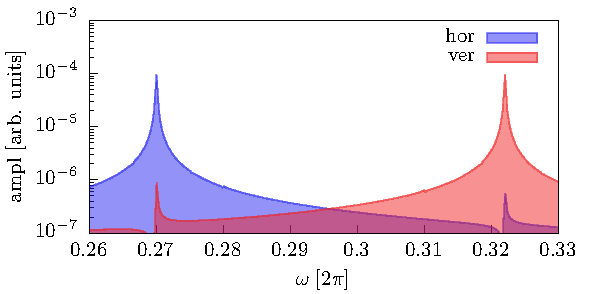
\includegraphics[width=0.8\linewidth]{figures/spectrum_plot}
    \caption{
        This example plot shows the Fourier transform of horizontal and vertical particle motion
        from simulations with an AC-dipole and coupling sources. The vertical and horizontal fractional 
        driven tunes are $Q_x^d=0.270$ and $Q_y^d=0.322$.
    }
    \label{fig_cplx_spctr}
\end{figure}
Figure~\ref{fig_cplx_spctr} shows the spectrum of $h_x^+$ and $h_y^+$ excited by an AC-dipole and with coupling.
The driven fractional tunes are $Q_x^d=0.270$ and $Q_y^d=0.322$. The respective main lines are well dominating the spectrum
and the secondary lines induced by coupling are clearly visible at the position of the respective other plane's tune.
For the following it is convenient to introduce a shorthand notation for the spectral lines $\four{h_z^\pm}(n_xQ_x+n_yQ_y)$:
%
\begin{align}
    H^\pm(n_x,n_y) &= \four{h_x^\pm}(n_xQ_x+n_yQ_y) \notag\\
    V^\pm(n_x,n_y) &= \four{h_y^\pm}(n_xQ_x+n_yQ_y) 
    \fstop
\end{align}
%
If the BPM calibration is not perfect the measured $H$ and $V$ lines are not proportional w.r.t. each other:
\newcommand{\meas}{^\text{meas}}
%
\begin{align}
   x\meas &= C_x x \notag \\ 
   y\meas &= C_y y
   \fstop
\end{align}
%
The calibration factors $C_{x/y}$ cancel out if one divides the spectral line by the amplitude of
the main line:
%
\begin{align}
    A_{0,n_y} &= \frac{H^+(0,n_y)}{\left|H^+(1,0)\right|} \notag \\
    B_{n_x,0} &= \frac{V^+(n_x,0)}{\left|V^+(0,1)\right|} 
    \fstop
\end{align}
%
Important for the coupling calculation are the following normalised spectral lines:
%
\begin{align}
    A_{0,1}&=\frac{H^+(0,1)}{\left|H^+(1,0)\right|}
      &= 2i\sqrt{\frac{J_y}{J_x}}\conj{f_{1001}} \e{-i\varphi_{y}}
    \label{eq_A01} \\
    B_{1,0}&=\frac{V^+(1,0)}{\left|V^+(0,1)\right|}
      &= 2i\sqrt{\frac{J_x}{J_y}}{f_{1001}} \e{-i\varphi_{x}}
    \label{eq_B10}
\end{align}
which contain $f_{1001}$ and
\begin{align}
    A_{0,-1}&=\frac{H^+(0,-1)}{\left|H^+(1,0)\right|}
      &= 2i\sqrt{\frac{J_y}{J_x}}\conj{f_{1010}} \e{i\varphi_{y}}
    \label{eq_A0-1} \\
    B_{-1,0}&=\frac{V^+(-1,0)}{\left|V^+(0,1)\right|}
      &= 2i\sqrt{\frac{J_x}{J_y}}\conj{f_{1010}} \e{i\varphi_{x}}
    \label{eq_B-10}
\end{align}
%
which contain $f_{1010}$.

The coupling RDTs $f_{1010}$ and $f_{1001}$ can then be calculated by combining Eqs~(\ref{eq_A01}) with (\ref{eq_B10})
and Eqs~(\ref{eq_A0-1}) with (\ref{eq_B-10}), respectively:
%
\begin{align}
    \left|f_{1001}\right| &= \frac{1}{2}\sqrt{\left| A_{0,1}B_{1,0} \right|} \notag \\
    \left|f_{1010}\right| &= \frac{1}{2}\sqrt{\left| A_{0,-1}B_{-1,0} \right|}
    \label{eq_abs_f_from_AB}
    \fstop
\end{align}
%
The normalised spectral lines $A_{0,n_y}$ and $B_{n_x,0}$ are the Fourier components of the complex
coordinates. But only the projections onto the real axis can be measured. The next step is to calculate
the complex coordinates from the measured ones.

Since $h_z^\pm = z \pm ip_z$ the complex coordinate can be obtained from position and momentum.
BPMs can only measure position but using the position data from a second BPM one can reconstruct the momentum.
The propagation of complex C-S coordinates through a region that is empty of non-linearities reads
%
\begin{equation}
    \begin{pmatrix}
        \hat{z}\\ \hat{p}_z
    \end{pmatrix}_b = \mat{R}_{ab} 
    \begin{pmatrix}
        \hat{z}\\ \hat{p}_z
    \end{pmatrix}_a
\end{equation}
%
where the transfer matrix $\mat{R}_{ab}$ is a simple rotation matrix as discussed in section~\ref{sec_intro_cs}.
From this one can reconstruct the momentum:
%
\begin{equation}
    \hat{p}_a = \frac{\hat{x}_b}{\cos\phi_{ab}} + \hat{x}_a \tan\phi_{ab}
\end{equation}
%
where $\phi_{ab}$ is the phase advance between the two positions $s_a$ and $s_b$.
Therefore:
%
\begin{equation}
    h_z^\pm(s_a) = \hat{z}_a - i \left(\frac{\hat{z}_b}{\cos\phi_{ab}} + \hat{z}_a\tan\phi_{ab} \right) = \hat{z}_a(1-i\tan\phi_{ab}) - i \frac{\hat{z}_b}{\cos\phi_{ab}}
    \fstop
\end{equation}
%
Since the Fourier transform is linear, this identity can be propagated to the spectral lines:
%
\begin{equation}
    H^+(n_x,n_y)_a = (1-i\tan\phi_{ab})H(n_x,n_y)_a - \frac{i}{\cos\phi_{ab}}H(n_x,n_y)_b
    \label{eq_reconstr_cplx}
\end{equation}
where $H(n_x,n_y)$ is the measured spectral line which is just the real projection of the complex line. 
%
Under the assumption that the region between $s_a$ and $s_b$ is free from non-li\-nea\-ri\-ties and coupling
the action $J_z$ does not change between the two positions and
%
\begin{align}
    |H(1,0)_a| &= |H(1,0)_b| = \sqrt{2J_x} \notag\\
    |V(0,1)_a| &= |V(0,1)_b| = \sqrt{2J_y}
    \fstop
\end{align}
%
This allows to express the real normalised spectral lines as
%
\begin{align}
    A(0,n_y)_a &= \frac{H(0,n_y)_a}{\left| H(1,0)_a \right|} = \frac{H(0,n_y)_a}{\left| H(1,0)_b \right|} \notag \\
    B(n_x,0)_a &= \frac{V(n_x,0)_a}{\left| V(0,1)_a \right|} = \frac{V(n_x,0)_a}{\left| V(0,1)_b \right|} 
    \fstop
\end{align}
%
This can be plugged into the reconstruction formula \eqref{eq_reconstr_cplx}
%
\begin{equation}
    \frac{H^+(n_x,n_y)_a}{H(1,0)_i} = (1-i\tan\phi_{ab})A(n_x,n_y)_a - \frac{i}{\cos\phi_{ab}}A(n_x,n_y)_b
    \label{eq_reconstr_from_norm}
\end{equation}
%
Together with the identity
%
\begin{equation}
    H(1,0) = \frac{1}{2} \left( H^+(1,0) + {H^-(1,0)}\right) = \frac{1}{2}H^+(1,0)
\end{equation}
%
because $H^-(1,0) = 0$, one can express $A^+(0,n_y)$ and $B(n_x, 0)$ in terms of normalised real spectral lines
%
\begin{align}
    2A^+(n_x,n_y)_a = (1-i\tan\phi_{ab})A(n_x,n_y)_a - \frac{i}{\cos\phi_{ab}}A(n_x,n_y)_b \notag \\
    2B^+(n_x,n_y)_a = (1-i\tan\phi_{ab})B(n_x,n_y)_a - \frac{i}{\cos\phi_{ab}}B(n_x,n_y)_b
    \label{eq_recon_AB}
\end{align}
%

Which can now be plugged in Eq~(\ref{eq_abs_f_from_AB}) to calculate the amplitude of the coupling RDTs
$f_{1001}$ and $f_{1010}$. To get the phase the starting point is, again, Eqs~(\ref{eq_A01}) -- (\ref{eq_B-10}).
The phases of $A_{0.1},\,B_{1,0},\,A_{0,-1},\,B_{-1,0}$ contain the phases of the RDTs:
%
\begin{align}
  \text{arg}(A_{0,1}) &= -q_{1001} -\varphi_y +\tfrac{\pi}{2} \\
  \text{arg}(B_{1,0}) &= q_{1001} -\varphi_x +\tfrac{\pi}{2} \\
  \text{arg}(A_{0,-1}) &= -q_{1010} +\varphi_y +\tfrac{\pi}{2} \\
  \text{arg}(B_{-1,0}) &= -q_{1010} +\varphi_x +\tfrac{\pi}{2}
  \label{eq_argA10B01}
\end{align}
%
where the phase $\frac{\pi}{2}$ comes from the factor $i$ and the phases of the RDTs are defined as
%
\begin{align}
  q_{1001} &\equiv \text{arg}(f_{1001})\\
  q_{1010} &\equiv \text{arg}(f_{1010})
  \fstop
  \label{eq_arg_f1001}
\end{align}
%
From \eqref{eq_argA10B01} one gets two expressions for each RDT phase:
%
\begin{equation}
  \begin{matrix*}[l]
  q_{1001} &= -\arg{A_{0,1}}-\varphi_y + \tfrac{\pi}{2} &= \arg{B_{1,0}}+\varphi_x -\tfrac{\pi}{2}\\
  q_{1010} &= -\arg{A_{0,-1}} +\varphi_y + \tfrac{\pi}{2} &= -\arg{B_{-1,0}}+\varphi_x +\tfrac{\pi}{2}
  \label{eq_q1001q1010}
  \end{matrix*}
\end{equation}
%
which can finally be used to calculate the RDTs using \eqref{eq_abs_f_from_AB}.

% --------------------------------------------------------------------------------------------------
% --------------------------------------------------------------------------------------------------
% Forced motion
% --------------------------------------------------------------------------------------------------
\section{Forced motion}

This section will introduce the process of optics measurements with an AC-dipole. As stated above,
the effect of the driving of the beam motion has to be compensated and the foundation for this
compensation will be explained in the following subsections.

% --------------------------------------------------------------------------------------------------
% Linear motion with AC dipole
% --------------------------------------------------------------------------------------------------
\subsection{Linear motion with AC dipole}
\newcommand{\Qd}[1]{Q^{d}_{#1}}
\label{sec_driven_coords}

In this section the C-S coordinates of the driven linear motion will be derived \cite{Miyamoto2010,Peggs1998}. These forced coordinates
can be used to calculate the effect of the AC dipole on linear optics parameters like betatron phase, 
$\beta$~function and linear transverse coupling.

At each turn an AC dipole located at position $s_d$ inflicts a kick to the beam. This kick can be
described in Courant-Snyder coordinates as
%
\begin{equation}
    \Delta h_z^+(N) = i A_\theta\beta(s_d) \cos(2\pi \Qd{z} N)
    \label{eq_ackick}
\end{equation}
%
depending on the AC dipole frequency $\Qd{z}$ and the turn number $N$. Figure~\ref{fig_ac_kick} shows
a schematic of the beam deflection for several turns.
%
\begin{figure}[ht]
    \centering
    \includestandalone{figACkick}
    \caption{
        Schematic of an AC-dipole kick. The deflection $\Delta p_z = A_\theta\beta(s_d)\cos(2\pi i Q_z N)$
        changes with turn number $N$.}
    \label{fig_ac_kick}
\end{figure}
%
At a small distance $\epsilon$ after the AC-dipole the C-S coordinates of the beam read
%
\begin{equation}
    h_z^+(s_d + \epsilon, N=0) = h_z^+(s_d-\epsilon) + \Delta h_z^+(N=0)
    \label{eq_ackick_at_epsilon}
\end{equation}
%
in the first turn where the AC dipole is active. This turn will be denoted with $N=0$.

Under the assumption that the kick strength of the AC-dipole is ramped up slowly enough, this is an
adiabatic process and the effect of the kicks can be added repeatedly for each turn.
The coordinates can be propagated to an arbitrary position $s$ in the ring to get the following
expressions:
%
\begin{align}
    h_z^+(s<s_d, N) &= R_{s-s_d}\left[R^N h_z^+(s_d) + R^N\Delta h_z^+(0) + \ldots + R\Delta h_z^+(N-1)\right] \notag\\
    h_z^+(s>s_d, N) &= R_{s-s_d}\left[R^N h_z^+(s_d) + R^N\Delta h_z^+(0) + \ldots + R\Delta h_z^+(N-1) + \Delta h_z^+(N)\right] 
    \komma\\
    h_z^+(s<s_d, N) &= R_{s-s_d}\left[R^N h_z^+(s_d) + \sum\limits_{T=1}^N R^T\Delta h_z^+(N-T)\right] \notag\\
    h_z^+(s>s_d, N) &= R_{s-s_d}\left[R^N h_z^+(s_d) + \sum\limits_{T=0}^N R^T\Delta h_z^+(N-T)\right]
    \komma
    \label{eq_hz_ackick}
\end{align}
%
with $R$ being the rotation map of the linear motion. For simplicity, the following definition has been used:
%
\begin{align}
    &R_{s-s_d} \equiv R(\varphi(s) - \varphi(s_d))\\
    \Rightarrow &R_{s-s_d} h_x = h_x \e{-i\varphi_{s_d s}}
    \fstop
\end{align}
%
\begin{figure}
    \centering
    \includestandalone{ac_kick_at_eps} 
    \caption{
        Schematic showing the positions and length occuring in \eqref{eq_ackick_at_epsilon}.
        The AC-dipole is located at position $s_d$.
        The beam gets a kick when passing from $s_d - \varepsilon$ to $s_d + \varepsilon$.
    }
\end{figure}
%
The cosine in \eqref{eq_ackick} can be expressed in complex form
%
\begin{align}
    \Delta h_z^+(N) &= \frac{iA_\theta\beta(s_d)}{2} \left(
        \e{2\pi i \Qd{z} N} +
        \e{-2\pi i \Qd{z} N}
    \right) \notag\\
    &= \frac{iA_\theta\beta(s_d)}{2} \left(
        \delta_+^N + \delta_-^N
    \right)
    \komma
\end{align}
%
where $\delta_\pm$ is defined as
%
\begin{equation}
    \delta_\pm = \e{\pm 2\pi i \Qd{z}}
    \fstop
\end{equation}
%
Using the complex form of the cosine, the kick in \eqref{eq_hz_ackick} can be split into left and right moving parts:
%
\begin{multline}
    h_z^+(s>s_d, N) = \\
    R_{s-s_d}\left[
        R^N h_z^+(s_d) +
        \frac{iA_\theta\beta(s_d)}{2}\left\{
            \sum\limits_{T=0}^N R^T \delta_+^{N-T}
            + \sum\limits_{T=0}^N R^T \delta_-^{N-T}
        \right\}
        \right]
    \fstop
\end{multline}
%
For the next simplification it shall be noted that
%
\begin{equation}
    \sum\limits_{i=0}^n x^i = \sum\limits_{i=n}^0 x^i = \sum\limits_{j=0}^{n} x^{n-j}
    \fstop
\end{equation}
%
The first transformation is a simple exchange in summation limits. The second one arises from the
change $i\rightarrow j=N-i$ and, thus, $j_0 = N-i_0 = 0$ and $j_1 = N - i_1 = 0$.
Using this, the sums can be brought into the form of a geometric series
%
\begin{align}
    \sum\limits_{T=0}^N R^T\delta_\pm^{N-T}
    &= \sum\limits_{T=0}^N R^{N-T}\delta_\pm^{T} \notag \\
    &=  R ^N \sum\limits_{T=0}^N \left( R^{-1}\delta_\pm \right)^{T} \notag \\
    &=  R ^N \frac{1- (R^{-1}\delta_\pm)^{N+1}}{1 - R^{-1}\delta_\pm}
    \komma
\end{align}
%
and
%
\begin{align}
    \sum\limits_{T=1}^N R^T\delta_\pm^{N-T}
    &= R^N \frac{1- (R^{-1}\delta_\pm)^{N}}{1 - R^{-1}\delta_\pm}
    \fstop
\end{align}
%
The two cases of \eqref{eq_hz_ackick} differ only in one additional exponent of $R^{-1}\delta_\pm$
and it can be written compactly as
%
\begin{align}
    h_z^+(s, N) = R_{s-s_d}R^N 
    \Bigg[&h_z^+(s_d)  \notag \\
        &+ \frac{iA_\theta\beta(s_d)}{2}\frac{1-(R^{-1}\delta_+)^{N+\Theta(s,s_d)}}{1-R^{-1}\delta_+}  \notag \\
        &+ \frac{iA_\theta\beta(s_d)}{2}\frac{1-(R^{-1}\delta_-)^{N+\Theta(s,s_d)}}{1-R^{-1}\delta_-}
    \Bigg]
    \fstop
\end{align}
%
Furthermore, the terms $R\delta_\pm$ can be written out:
%
\begin{equation}
    R^{-1}\delta_\pm = \e{2\pi i (Q_z \pm \Qd{z})} = \e{\pm 2\pi i Q_z^\pm}
    \komma
\end{equation}
%
and
%
\begin{equation}
    1 - \e{2i\alpha} = -\e{i\alpha}2i \sin\alpha
    \fstop
\end{equation}
%
Those identities can be used to simplify the exponentials
%
\begin{align}
    h_z^+(s, N) = R_{s-s_d}R^N 
    \Bigg[&h_z^+(s_d)  \notag \\
        &+ \frac{A_\theta\beta(s_d)}{4}\frac{1-\e{2\pi i Q_z^+(N+\Theta(s,s_d))}}{\e{i\pi Q_z^+}\sin\left( \pi Q_z^+ \right)}  \notag \\
        &- \frac{A_\theta\beta(s_d)}{4}\frac{1-\e{-2\pi i Q_z^-(N+\Theta(s,s_d))}}{\e{i\pi Q_z^-}\sin\left( \pi Q_z^- \right)}
    \Bigg]
    \fstop
    \label{eq_delta_written_out}
\end{align}
%
The term $h_z^+$ in \eqref{eq_delta_written_out} can be put into 
%
\begin{equation}
    \tilde{h}_z^+(s_d) \equiv h_z^+(s_d) + 
    \left(
    \frac{A_\theta\beta(s_d)}{4\sin\left( \pi Q_z^-\right)}\lambda_z \e{i \pi Q_z^-}
    -\frac{A_\theta\beta(s_d)}{4\sin\left( \pi Q_z^+\right)} \e{-i\pi Q_z^+}
    \right)
    \fstop
\end{equation}
%
Now, the driven motion is seperated off:
%
\begin{align}
    h_z^+(s, N) = R_{s-s_d}R^N 
    \Bigg[&\tilde{h}_z(s_d) 
    \notag \\
        &+ \frac{A_\theta\beta(s_d)}{4\sin\left( \pi Q_z^-\right)} \e{-\pi i Q_z^-(2N+2\Theta(s,s_d)-1)} 
         \notag \\
        &- \frac{A_\theta\beta(s_d)}{4\sin\left( \pi Q_z^+\right)} \e{\pi i Q_z^+(2N+2\Theta(s,s_d) -1)}
    \Bigg]
    \fstop
    \label{eq_driven_simpl_R}
\end{align}
%
and the linear rotation can be integrated into the terms:
%
\begin{align}
    h_z^+(s, N) =
        &\tilde{h}_z(s, N) \notag \\
        &+\frac{A_\theta\beta(s_d)}{4\sin\left( \pi Q_z^-\right)}
        \e{i\left[-2\pi NQ_{z} - \varphi_{s_ds} + \pi Q_z^-(2N+2\Theta(s,s_d)-1)\right]}
        \notag\\
        &-\frac{A_\theta\beta(s_d)}{4\sin\left( \pi Q_z^+\right)}
        \e{i\left[2\pi NQ_{z} - \varphi_{s_ds}- \pi Q_z^+(2N + 2\Theta(s,s_d) -1)\right]}
    \fstop
    \label{eq_driven_simpl}
\end{align}
%
Noting that
%
\begin{equation}
  2\Theta(a) - 1 = \text{sgn}(a) \text{, if } a \neq 0
    \komma
\end{equation}
%
\eqref{eq_driven_simpl} can be further simplified\footnote{
    strictly speaking \eqref{eq_driven_simpl2} is valid only for $s\neq s_d$ and one should carefully exclude this case
    in the following. But since a measurement at the exact position of the AC Dipole is not possible in the first place
    this fine detail will be ignored in this work.
    }:
%
\begin{align}
    h_z^+(s, N) =
        &\tilde{h}_z(s, N) \notag \\
        &+ \frac{A_\theta\beta(s_d)}{4\sin\left( \pi Q_z^-\right)}
        \e{i\left[-2N\pi \Qd{z} - \varphi_{s_ds} + \pi Q_z^-\text{sgn}(s-s_d)\right]} 
        \notag \\
        &- \frac{A_\theta\beta(s_d)}{4\sin\left( \pi Q_z^+\right)}
        \e{i\left[2N\pi \Qd{z} - \varphi_{s_ds} - \pi Q_z^+\text{sgn}(s-s_d)\right]} 
    \fstop
    \label{eq_driven_simpl2}
\end{align}
%
The free motion of the beam is perturbed by two driving modes corresponding to the sum and difference
of natural tune and driven tune. In most applications the ac-dipole strength is much greater than the free 
oscillation amplitude $A_\theta\beta(s_d) \gg |\bar{h}_z(s,N)|$.

All derivations in this section have been made for $h_z^+$. It shall be noted here that the negatively turning
coordinate $h_z^-$ has the form
%
\begin{align}
    h_z^-(s, N) =
        &\tilde{h}_z^-(s, N) \notag \\
        &+ \frac{A_\theta\beta(s_d)}{4\sin\left( \pi Q_z^-\right)}
        \e{i\left[2N\pi \Qd{z} + \varphi_{s_ds} - \pi Q_z^-\text{sgn}(s-s_d)\right]} 
        \notag \\
        &- \frac{A_\theta\beta(s_d)}{4\sin\left( \pi Q_z^+\right)}
        \e{i\left[-2N\pi \Qd{z} + \varphi_{s_ds} + \pi Q_z^+\text{sgn}(s-s_d)\right]} 
    \fstop
    \label{eq_driven_simpl2_minus}
\end{align}
%
Subtracting the closed driven closed orbit $\tilde{h}_z$ and with the definition
%
\begin{equation}
    \lambda_z = \frac{\sin(\pi Q_z^-)}{\sin(\pi Q_z^+)}
    \komma
\end{equation}
%
the driven motion can be rewritten in the from
%
\begin{align}
    h_z^\pm(s,N) = 
        \frac{A_\theta\beta(s_d)}{4\sin\left( \pi Q_z^-\right)}
        \Bigg[ 
            &\e{\pm i\left[-2N\pi \Qd{z} - \varphi_{s_ds} + \pi Q_z^-\text{sgn}(s-s_d)\right]} 
            \notag \\
            &- \lambda_z
             \e{\pm i\left[2N\pi \Qd{z} - \varphi_{s_ds} - \pi Q_z^+\text{sgn}(s-s_d)\right]} 
        \Bigg]
    \komma
    \label{eq_driven_hz_final}
\end{align}
%
which is used in other works \cite{Miyamoto2008, Miyamoto2010}. 

% --------------------------------------------------------------------------------------------------
% Compensation
% --------------------------------------------------------------------------------------------------
\subsection{Compensation of linear parameters}
\label{sec_comp}

This section briefly summarises the compensation of the driven motion for the optics parameters
$\beta$, $\alpha$ and $\phi$ \footnote{\cite{Miyamoto2008} and Ryoichi Miyamoto, private communication, Feb. 2017}.

In an actual measurement the phase and amplitude are calculated from the Fourier analysis of the
real signal.
%
\begin{align}
   H(1,0)^\text{free} &= \frac{1}{2}\left( H^+(1,0)^\text{free} + H^-(1,0)^\text{free} \right)\notag \\
   &= \sqrt{2 J_z\beta} \left[ \e{-i\varphi(s) } + \e{i\varphi(s)} \right]
   \label{eq_four_real_free}
\end{align}
%
for the free motion and
%
\begin{align}
   H(1,0)
   % &= \notag \\
   &= \frac{A_\theta\beta(s_d)}{4\sin(\pi Q_z^-)}\left[
        \e{i\left[-\varphi_{s_ds} + \pi Q_z^-\text{sgn}(s_ds)\right]}
        -\lambda \e{i\left[\varphi_{s_ds} + \pi Q_z^+\text{sgn}(s_ds)\right]}
       \right]
       \label{eq_four_real_driven}
\end{align}
for the driven motion.
%
For the next steps the following trigonometric reformulation is needed:
%
\begin{equation}
  \e{i\left( \alpha + \beta \right)} - \lambda \e{i\left( \alpha - \beta \right)}
  = \e{i\alpha} \left(\e{i\beta} - \lambda\e{-i\beta}\right)
  \fstop
  \label{eq_e_alpha_lambda}
\end{equation}
%
The sum of two oscillations with the same frequency forms a single oscillation, so the $\beta$~term can
be rewritten as
%
\begin{equation}
  B = |B|\e{i\psi}
\end{equation}
with
%
\begin{align}
  |B|^2 &=  \left( \e{i\beta}-\lambda\e{-i\beta} \right)\left( \e{-i\beta} - \lambda\e{i\beta} \right)
  = 1+\lambda^2-2\lambda\cos{2\beta} \notag \\
  \psi&= \atan \frac{\im{B}}{\re{B}} = \atan\left(\frac{1+\lambda}{1-\lambda}\tan \beta\right)
  \fstop
\end{align}
%
Now \eqref{eq_four_real_driven} can be put in this form by defining
%
\begin{align}
  \alpha &\equiv \pi\Qd{z} \text{sgn}(s-s_d) \notag \\
  \beta &\equiv \pi Q_z\text{sgn}(s-s_d) - \varphi_{s_ds}
\end{align}
%
This allows for $H(1,0)$ to be rewritten
%
\begin{align}
  H(1,0) =&\: \frac{A_\theta\beta(s_d)}{4\sin(\pi Q_z^-)}
      \sqrt{1+\lambda^2-2\lambda\cos\left[2\varphi_{s_ds} - \pi Q_z\text{sgn}(s-s_d)\right]} \notag \\
      &\times\e{i\left[ \pi \Qd{z}\text{sgn}(s-s_d) + \psi \right]}
  \fstop
  \label{eq_H_drv}
\end{align}
%
Comparing to the free case, \eqref{eq_four_real_free}, the driven phase is defined as 
%
\begin{align}
  \varphi^d_{s_ds} &=  \Qd{z}\text{sgn}(s-s_d) + \psi\notag\\
  &=  \Qd{z}\text{sgn}(s-s_d)
  + \atan\left( \frac{1+\lambda}{1-\lambda}\tan\left( \varphi_{s_ds}-\pi Q_z\text{sgn}(s-s_d)\right) \right)
\end{align}
%
which fullfils the symmetric property
%
\begin{equation}
  (1-\lambda)\tan\left( \varphi^d_{s_ds} -\pi \Qd{z}\text{sgn}(s-s_d) \right)
  =
  (1+\lambda)\tan\left( \varphi_{s_ds} -\pi Q_z\text{sgn}(s-s_d) \right)
  \label{eq_drv_phase_sym}
\end{equation}
%
In order to get the driven Twiss parameters $\alpha^d$, $\beta^d$ and $\gamma^d$, the same relation
between them and the driven phase $\varphi^d$ is imposed:
\begin{equation}
  \frac{\der \varphi^d}{\der s} = \frac{1}{\beta^d}
\end{equation}
%
Taking the derivative of  \eqref{eq_drv_phase_sym} w.r.t. $s$ yields
%
\begin{equation}
  \frac{(1-\lambda)\varphi'^d(s)}{\cos^2\left[ \varphi^d(s) - \pi\Qd{z}\text{sgn}(s-s_d) \right]}
  =
  \frac{(1+\lambda)\varphi'(s)}{\cos^2\left[ \varphi(s) - \pi Q_z\text{sgn}(s-s_d) \right]}
  \komma
\end{equation}
%
where it is assumed that all phases are w.r.t. the position of the AC-dipole $s_d$ and $f'(x)$ denotes
the derivative of the function $f$ with respect to $x$.
Respectively, taking its square yields
\begin{equation}
  \frac{(1-\lambda)}{\cos^2\left[ \varphi^d(s) - \pi\Qd{z}\text{sgn}(s-s_d) \right]} +2\lambda
  =
  \frac{(1+\lambda)^2}{\cos^2\left[ \varphi(s) - \pi Q_z\text{sgn}(s-s_d) \right]} -2\lambda
  \fstop
  \label{<+label+>}
\end{equation}
%
Both equations can be used to cancel $\cos\left[ \varphi^d(s) - \pi \Qd{z}\text{sgn}(s-s_d) \right]$:
%
\begin{equation}
  \frac{1}{\varphi'^d(s)} = 
  \frac{1+\lambda^2-2\lambda\cos\left[ 2\varphi(s) - 2\pi Q_z\text{sgn}(s-s_d)\right]}{1-\lambda^2}
  \frac{1}{\varphi'(s)}
\end{equation}
%
which, finally, is the formula to compute the driven $\beta$~function:
%
\begin{equation}
  \beta^d(s) =
  \frac{1+\lambda^2-2\lambda\cos\left[ 2\varphi(s) - 2\pi Q_z\text{sgn}(s-s_d)\right]}{1-\lambda^2}
  \beta(s)
\end{equation}
%
The driven $\alpha$ function follows from the definition of the free $\alpha$~function:
\begin{align}
  \alpha^d(s) &=  \frac{1}{2}\frac{\der \beta^d}{\der s}\notag \\
  &= 
  \frac{1+\lambda^2-2\lambda\cos\left[ 2\varphi(s) - 2\pi Q_z\text{sgn}(s-s_d)\right]}{1-\lambda^2}
  \alpha(s) \notag \\
  &\quad- 2\lambda \sin\left[ 2\varphi(s) - 2\pi Q_z\text{sgn}(s-s_d) \right]
  \label{eq_drv_alpha}
\end{align}
%
Comparing the amplitude of the driven motion \eqref{eq_H_drv} with the amplitude of \eqref{eq_four_real_free}
the driven action $J_x^d$ can be deduced:
%
\begin{align}
  \sqrt{2J_z^d\beta_z^d(s)} &= 
  \frac{A_\theta\sqrt{\beta(s_d)\beta(s)}}{4\sin(\pi Q_z^-)}
  \sqrt{1+\lambda^2-2\lambda\cos\left[2\varphi_{s_ds} - \pi Q_z\text{sgn}(s-s_d)\right]} \notag \\
  \Rightarrow J_z^d &=  \frac{A_\theta^2\beta(s_d)(1-\lambda^2)}{32 \sin^2(\pi Q_z^-)}
  \fstop
  \label{eq_drv_Jy}
\end{align}
%
The expressions for the driven optics parameters $\beta^d$, $\alpha^d$, $\varphi^d$ and $J^d$ derived
in this section can be used to compensate for the effect of the driven motion on the measurement and enable
an easy measurement leveraging the advantages of an AC-dipole for optics measurements in circular
accelerators.


\chapter{The Analytical N-BPM method}
\label{ch_anbpm}

\begin{chapterinfo}
One of the most important figures of merit of optics correction is the deviation of the real $\beta$~function
from the model values,
the $\beta$~\emph{beating}. A deviation from the ideal values has a negative effect on machine performance.
Too high $\beta$~beating can even put machine components in danger and a threshold for operation with
physics filling scheme has to be imposed for machine protection reasons.

Furthermore, large $\beta$~beating deteriorates other linear and especially non-linear optics measurements
and correction methods. Therefore a good control of the $\beta$~beating can be essential for higher-order
correction steps.

This chapter summarises classical $\beta$~beating methods from turn-by-turn data in section~\ref{sec_classical_beta_meas}
and describes in detail a new algorithm, the \emph{analytical N-BPM method},
which improves speed and performance by calculating analytically the error propagation
in sections~\ref{sec_corrected_beta_from_phase} through \ref{sec_corr_matr}.
Accuracy and precision of the new method are assessed using simulations of current LHC optics and design
optics for the High-Luminosity upgrade of the LHC in sections~\ref{sec_bad_combs} and \ref{sec_hllhc_nbpm}.

With the exception of the first two sections, which set the context of the present study and introduce the
mathematical tools, this chapter represents original work.

The content of this chapter has been published in~\cite{Wegscheider2017}.

\end{chapterinfo}

\section{\texorpdfstring{$\beta$}{beta}~function measurement from turn-by-turn data}
\label{sec_classical_beta_meas}

\subsection{Three BPM method}

The classical method to measure the $\beta$~function in hadron machines is the \emph{Three BPM Method}
introduced in section~\ref{sec_beta_meas}.



With this method one can use the phase advance between three BPMs $i,j,k$ to calculate the $\beta$~function
of the probed BPM $i$. It is a model dependent approach, the greater the difference between the model
and the real accelerator the less accurate will be the result. A good knowledge of the actual accelerator
is crucial for this approach to work.

\equationref{eq_3bpm_method} has been developped for LEP and it has been used for optics measurements in LEP
and LHC during run I.
But it has two shortcomings: it assumes that the actual $\beta$~beating is very low and it
diverges for phase advances close to $n\pi$, $n \in \mathbb{N}$. The latter makes measurements at
exact $n\pi$ phase advances impossible and strongly enhances phase measurement errors near $n\pi$.
Unfortunately especially in the IR phase advances are very small and precise $\beta$~function measurements
are not feasible.

%\begin{wrapfigure}{O}[\figborderhang]{6cm}
\begin{figure}
    \centering
    \includestandalone{figThreeBPM} 
    \caption{A sketch of the three BPM method. The probed BPM is shown in blue. For LHC arcs the
    combination with the probed BPM in the center is the most stable against phase measurement errors.}
    \label{fig_threebpm}
\end{figure}
%
\figureref{fig_threebpm} displays a sketch of the Three BPM Method. The probed BPM is shown in blue,
BPMs $j$ and $k$ are shown in red.
Classically the arithmetic mean of all three adjacent cases -- as shown in the figure -- were used.


In LHC arcs where the phase advance between adjacent BPMs is around
$\SI{45}{\degree}$ the combination with the probed BPM in the center yields almost optimal results
since the perturbation from phase measurement errors is small for the occurring phase advances.
The two other cases shown in \figref{fig_threebpm} on the other hand include the 
phase advance $\phi_{13} = \SI{90}{\degree}$ which is less optimal.

In LHC interaction regions the phase advance between consecutive BPMs does not follow the same constraints
as in the arc and values different from $\SI{45}{\degree}$ may appear. In the final focus quadrupoles
the $\beta$~function peaks are very high to deliver a strong focusing of the beams in the interaction
point. This yields a very small phase advance in this area, rendering a $\beta$ measurement from phase
impossible. At the same time a high precision of $\beta$~beating is necessary to control $\betastar$ and
to optimise the aperture.

\subsection{Original N-BPM method}

To avoid cases with unsuitable phase advances or to get the optimal phase advances, BPMs can be
skipped. For an LHC arc a combination as shown in \figref{fig_skip_one_BPM} can be used for the non-center
cases of the Three BPM method in order to have the least uncertainties in all three combinations.

A second tool that can be applied to reduce uncertainty is averaging over more combinations which
improves statistics and reduces statistical uncertainties.
Unfortunately, systematic errors increase
as more and more BPMs are skipped because of the presence of other elements with their imperfections in between the
BPMs.
In order to further improve the precision the information about statistical and systematic
uncertainties can be used to calculate a weighted mean. 
%
\begin{align}
    \beta(s_i) &= \sum\limits_{l} \beta_l(s_i) g_l
    \label{eq_beta_wmean}\\
    \beta_l(s_i) &= \frac{\cot\phi_{ij_l} - \cot\phi_{ik_l}}{\cot\phi_{ij_l}\m - \cot\phi_{ik_l}} \beta(s_i)\m
    \label{eq_beta_l}
\end{align}
%
with the weights $g_l$ satisfying
%
\begin{equation}
    \sum\limits_l g_l = 1
\end{equation}
%
and $j_l,\,k_l$ pairs of BPMs around the probed BPM.


%\begin{wrapfigure}{O}[\figborderhang]{7cm}
\begin{figure}
    \centering
    \includestandalone{figSkipOneBpm}
    \caption{In the LHC arcs skipping one BPM for the non-center cases of the Three BPM Method
    is of advantage since the phase advance $\phi_{14}$
    is more suitable regarding error propagation.}
    \label{fig_skip_one_BPM}
\end{figure}
%
Furthermore the $\beta$~function values calculated from different combinations are not statistically
independent and correlation has to be taken into account when calculating the weights.
The N-BPM method \cite{LangnerNBPM, Langner2017} was developped to implement this feature.
It was successfully used in the LHC during run II and for the re-analysis of run I data
as well as in the storage rings of ALBA and ESRF.

The name originates in the fact that the BPMs $i$, $j_l$ and $k_l$ are taken in a range of $N$ BPMs.
This generates $n = (N-2)(N-1)/2$ combinations.

% --------------------------------------------------------------------------------------------------
% Generalised least squares
% --------------------------------------------------------------------------------------------------
\section{Generalised least squares}

To get the correct estimate for the weights $g_l$ the study of some statistics is in order.
The weights can be determined using a least-squares optimisation. The weighted mean \eqref{eq_beta_wmean}
can be rewritten in vector notation:
%
\begin{align}
    \vec{\hat{\beta}} &= \mat{B}\vec{\gamma}
    \label{eq_beta_wmean_vec}\\
    \vec{\hat{\beta}} &= 
    \begin{pmatrix}
        \hat{\beta}\\
        \vdots\\
        \hat{\beta}
    \end{pmatrix},\quad
    \vec{\gamma} =
    \begin{pmatrix}
        g_1\\
        \vdots\\
        g_n
    \end{pmatrix},\quad
    \mat{B} =
    \begin{pmatrix}
        \vec{\beta}^T\\
        \vdots\\
        \vec{\beta}^T
    \end{pmatrix}
\end{align}
%
where each line of the equation system is just the same.
The difference between measurement $l$ and the mean value $\hat{\beta}$ is denoted by $\epsilon_l$:
%
\begin{equation}
    \vec{\epsilon} = \vec{\hat{\beta}} - \vec{\beta}
\end{equation}
%
The least square minimisation seeks a set of weights $g_i$ for which the squared errors are minimal. Since the different $\beta_l$
are correlated and have a covariance matrix $\mat{Cov}[\vec{\beta}] \neq \mat{diag}(\sigma_1^2, \ldots, \sigma_n^2)$
the theory of generalised least-squares estimation has to be applied.

The \emph{covariance matrix} of a set of random variables $\Omega_i$ is defined as
%
\begin{align}
    \mat{Cov}[\vec{\Omega}] &= \mat{E}[(\vec{\Omega} - E[\vec{\Omega}])(\vec{\Omega} - E[\vec{\Omega}])^T]
    \notag \\
    &= \mat{E}[\vec{\Omega}\vec{\Omega}^T] - E[\vec{\Omega}]E[\vec{\Omega}]^T
    \label{eq_def_cov}
\end{align}
%
where $E[\vec{\Omega}]$ is the \emph{expected value} of the random variables $\vec{\Omega}$. And the
notation is chosen such that the expected value of a vector is a vector
of expected values of each component and similar for matrices.

\equationref{eq_def_cov} can be expressed element-wise:
%
\begin{equation}
    \left(Cov[\vec{\Omega}]\right)_{ij} = E[\Omega_i\Omega_j] - E[\Omega_i]E[\Omega_j]
    \fstop
\end{equation}
%
\subsection{Error Propagation}

Consider a set of unperturbed phase measurements $ \{\phi_1, \ldots, \phi_n\} $ and non-observable  parameters $  \{ K_{1,1} , \ldots , K_{1,m}, s_1, \ldots, s_{\nu}, x_1, \ldots x_{\mu} \} $ with corresponding errors $ \Delta \phi_\alpha,\, \Delta K_{1,\beta}, \,\Delta s_\gamma,\, \Delta x_\kappa  $.
Collecting all parameters into a vector
%
\begin{equation}
\vec{\Omega}_0 =
\begin{pmatrix}
\vec{\phi}\\
\vec{K}\\
\vec{s}\\
\vec{x}
\end{pmatrix},\quad
\vec{\Delta \Omega} = 
\begin{pmatrix}
\vec{\Delta\phi}\\
\vec{\Delta K}\\
\vec{\Delta s}\\
\vec{\Delta x}
\end{pmatrix}.
\end{equation}
%
Using a Taylor expansion the errors in these parameters can be propagated
%
\begin{equation}
\beta_l (\vec{\Omega}) = \beta_l(\vec{\Omega}_0) + \partial^i\beta_l(\vec{\Omega}_0)\Delta\Omega_i +  \partial^i\partial^j\beta_l(\vec{\Omega}_0)\Delta\Omega_i\Delta\Omega_j + O(\Delta\Omega^3)\;,
\label{eq:err_prop}
\end{equation}
%
where the Einstein summation convention is used and the derivatives are w.r.t. $ \Omega_i $: $ \partial^i\beta_l \equiv \frac{\partial \beta_l}{\partial \Omega_i} $.
The argument $ (\vec{\Omega}_0) $ is omitted in the following for the $ \beta $ function and its derivatives at the unperturbed position $ \vec{\Omega}_0 $. For the calculation of the covariance matrix,
\eqref{eq:err_prop} is truncated to second order and derive the two summands of \eqref{eq_cov} separately.
%
\begin{equation}
E[\beta_l(\vec{\Omega})] \approx E\left[   
\beta_l + \partial^i\beta_l\Delta\Omega_i +  \partial^i\partial^j\beta_l\Delta\Omega_i\Delta\Omega_j 
\right] =
\beta_l + \partial^i\beta_l E[\Delta\Omega_i] +  \partial^i\partial^j\beta_l E\left[\Delta\Omega_i\Delta\Omega_j \right]\;.
\end{equation}
%
 It is assumed that there are no systematic errors in the measurement instruments and so $ {E}[{\Delta\Omega_i}] =0$ and the middle term vanishes.
One can conclude
%
\begin{equation}
E[\beta_l(\vec{\Omega})]E[\beta_m(\vec{\Omega})] \approx \beta_l\beta_m +
 \left(\beta_l\partial^i\partial^j\beta_m +
 \beta_m\partial^i\partial^j\beta_l\right) E\left[\Delta\Omega_i\Delta\Omega_j \right]\;,
 \label{eq:Eb_Eb}
\end{equation}
%
 where terms proportional to the square of the variance go into the reminder $ O(\Delta\Omega^3) $.

To calculate the term $ {E}[{\beta_l}{\beta_m}] $ more steps are needed:
%
\begin{align}
E\left[\beta_l(\vec{\Omega})\beta_m(\vec{\Omega})\right]& = 
E\left[
	(
		\beta_l + \partial^i\beta_l\Delta\Omega_i + \partial^i\partial^j\beta_l\Delta\Omega_i\Delta\Omega_j
	)
	(
		\beta_m + \partial^i\beta_m\Delta\Omega_i + \partial^i\partial^j\beta_m\Delta\Omega_i\Delta\Omega_j
	)
\right] \notag \\
&\approx E\left[
	\beta_l\beta_m + 
	\left(\beta_l\partial^i\beta_m + \beta_m\partial^i\beta_l\right)\Delta\Omega_i +
	\partial^i\beta_l\partial^j\beta_m\Delta\Omega_i\Delta\Omega_j +\right. \notag\\ &\left.\quad\quad\quad
	\left(\beta_l\partial^i\partial^j\beta_m +\beta_m\partial^i\partial^j\beta_l\right)\Delta\Omega_i\Delta\Omega_j
\right] \notag\\
&= 	
	\beta_l\beta_m + 
	\partial^i\beta_l\partial^j\beta_mE[\Delta\Omega_i\Delta\Omega_j]+
	\left(\beta_l\partial^i\partial^j\beta_m +
	\beta_m\partial^i\partial^j\beta_l\right) E\left[\Delta\Omega_i\Delta\Omega_j \right]\;.
	\label{eq:Ebb}
\end{align}
%
Finally, subtracting \eqref{eq:Eb_Eb} from \eqref{eq:Ebb}, yields
%
\begin{equation}
(\text{Cov}[\vec{\beta}])_{lm} = \partial^i\beta_l\partial^j\beta_mE[\Delta\Omega_i\Delta\Omega_j] = \partial^i\beta_l\partial^j\beta_m \text{Cov}[\vec{\Delta\Omega}]_{ij}\;.
\label{eq:covbb}
\end{equation}
%
In the last step again the assumption $ E(\Delta\Omega_i)=0 $ is made, implying
%
\begin{equation}\label{eq_cov}
\text{Cov}[\vec{\Delta\Omega}]_{ij} =  E\left[\Delta\Omega_i \right] E[\Delta\Omega_j ] -  E\left[\Delta\Omega_i\Delta\Omega_j \right] =  E\left[\Delta\Omega_i\Delta\Omega_j \right]\;.
\end{equation}
%
In matrix notation \eqref{eq:covbb} reads
%
\begin{equation}
\mat{Cov}\left[\vec{\beta}\right] = \mat{T}\; \mat{Cov}\left[\vec{\Delta\Omega}\right] \;\mat{T}^T,
\end{equation}
%
 where 
%
\begin{equation}
T_{ij} = \frac{\partial \beta_i}{\partial \Omega_j}\;.
\end{equation}
%
If the parameters $ \vec{\Omega} $ are uncorrelated, the covariance matrix of $\vec{ \Delta\Omega} $ simplifies to
%
\begin{align}
\left(\text{Cov}\left[\vec{\Delta\Omega}\right] \right)_{ij}&= 0 \quad  \text{ if } i\neq j \;,\\
 \left(\text{Cov}\left[\vec{\Delta\Omega}\right] \right)_{ii}&= \sigma_i^2\;,
\end{align}
%
%
\begin{equation}
\Rightarrow E\left[\Delta\Omega_i\Delta\Omega_j\right] = E\left[\Delta\Omega_i\right]E\left[\Delta\Omega_j\right]\quad \text{ if } i \neq j\;,
\end{equation}
%
and \eqref{eq:covbb} reads
%
\begin{equation}
(\text{Cov}[\vec{\beta}])_{lm} = \partial^i\beta_l\partial^i\beta_mE[\Delta\Omega_i^2] = \partial^i\beta_l\partial^i\beta_m \sigma_i^2\;,
\end{equation}
%
with the variance being defined by
%
\begin{equation}
\sigma_i^2 = E\left[\Delta\Omega_i^2\right].
\end{equation}
%
\subsection{The generalized least-squares estimator}

After computing the covariance matrix of $ \beta $, the generalized least-squares estimator can be calculated
by solving the translated system
%
\begin{equation}
\mat{X}^{-1} \vec{\beta} = \mat{X}^{-1}\mat{B}\vec{\gamma} + \mat{X}^{-1}\vec{\epsilon}
\end{equation}
%
where the translation $ \mat{X} $ is such that $ \mat{X}^T\mat{X} = \mat{V} = \mat{Cov}[\vec{\beta}] $. The least-squares estimation searches for a minimum of 
%
\begin{equation}
\left\|\mat{X}^{-1}\left(\vec{\beta} - \mat{B}\vec{\gamma}\right)\right\|^2 = \left(\vec{\beta} - \mat{B}\vec{\gamma}\right)^T \mat{V}^{-1}\left(\vec{\beta} - \mat{B}\vec{\gamma}\right)\;.
\label{eq:corr_syst}
\end{equation}
%
 %Deriving~(\ref{eq:corr_syst}) with respect to $ \vec{\gamma} $ yields
\eqref{eq:corr_syst} can be solved in the index notation:

\[\frac{\partial}{\partial g_k}\sum\limits_{i,j} \left(\beta_i - \sum_l\beta_lg_l\right) V_{ij}^{-1} \left(\beta_j-\sum_m\beta_mg_m\right) = 2\sum_{i,j}\beta_kV_{ij}^{-1}\left(\beta_j - \sum_m\beta_mg_m\right) = 0\]
%
\begin{align}
\Rightarrow \sum_{i,j}V_{ij}^{-1}\beta_j&=\sum_{i,j}V_{ij}^{-1}\sum_m\beta_mg_m\notag \\
\Rightarrow\sum_mg_m\beta_m &= \frac{\sum\limits_{i,j}V_{ij}^{-1}\beta_j}{\sum\limits_{i,j}V_{ij}^{-1}}=\sum_m \frac{\sum\limits_i V_{im}^{-1}}{\sum\limits_{i,j}V_{ij}^{-1}}\beta_m
\end{align}
%
 where the summation index can be renamed in the numerator to highlight a solution of the system:
%
\begin{equation}
g_i(\mat{V}) = \frac{\sum\limits_k V_{ik}^{-1}}{\sum\limits_{j,k}V_{jk}^{-1}}\; .
\end{equation}
%
The uncertainty of the weighted average is then
%
\begin{equation}
\sigma^2(\mat{X}^{-1}\vec{\beta}) = \vec{g}^T\mat{V}\vec{g} = \sum\limits_{i,j}g_iV_{ij}g_j\;.
\end{equation}
%
\subsection{Error matrix for N-BPM method}

The error matrix $ \mathbf{V} $ can be optained from the single variances by
%
\begin{equation}
\mathbf{V} = \mathbf{T}\mathbf{M}\mathbf{T}^{-1}\quad ,
\label{eq:V}
\end{equation}
%
where $ \mathbf{M}=\text{diag}(\sigma^2_{\phi_1}, \ldots, \sigma^2_{\phi_n}) $ is a diagonal matrix consisting of the variances of the phases and $ \mathbf{T} $ is the Jacobian matrix
%
\begin{equation}
T_{l\lambda}(s_i) = \left.\frac{\partial \beta_l(s_i)}{\partial \phi_\lambda} \right|_{\delta\phi=0}\quad ,
\label{eq:Tij}
\end{equation}
%
$ \delta\phi=0 $ meaning that the derivatives are evaluated with all phase advance errors set to zero. The correlation of statistical errors (coming from BPM noise) is
%
\begin{align}
&T_{l\lambda}^\phi(s_i) = \left.\frac{\partial \beta_l(s_i)}{\partial \phi_\lambda}\right|_{\delta \phi =0} =\notag\\ 
&\frac{
		\left(\delta_{i}^\lambda-\delta_{j_l}^\lambda\right)\sin^{-2}\phi\m_{i{j_l}} -
		\left(\delta_{i}^\lambda-\delta_{k_l}^\lambda\right)\sin^{-2}\phi_{i{k_l}}\m
	}
	{
		\cot \phi_{i{j_l}}\m - \cot\phi_{i{k_l}}\m
	}
\beta\m(s_i)\quad .
\label{eq:Tphiij}
\end{align}
%
A superscript $ \phi $ is placed here intentionally to highlight that the $ \mat{T} $ matrix only includes statistical errors coming from the uncertainty of the phase measurement. $\delta^\alpha_\beta $ denotes the Kronecker~$\delta$. Including systematic errors, the total error matrix is
%
\begin{equation}
\mathbf{V} = \mathbf{V_\text{stat}} + \mathbf{V}_\text{syst}\quad ,
\label{eq:V1}
\end{equation}
%
where $ \mathbf{V}_\text{stat} = \mathbf{T}^\phi \mathbf{M} {\mathbf{T}^{\phi}}^{-1}$ and the total uncertainty of the averaged $ \hat{\beta} $ is then given by
%
\begin{equation}
\sigma_{\hat{\beta}}^2 = \sigma_\text{stat}^2 + \sigma_\text{syst}^2\quad .
\end{equation}
%
\subsection{Extension of the N-BPM method}

In the existing numerical N-BPM method only the statistical errors are calculated analytically while
$\mathbf{V}_\text{syst}$ and hence $\sigma_\text{syst}^2$ are evaluated from Monte Carlo simulations
of lattices with errors.
For that the statistics over many simulations is gathered.
Even with a highly parallelized code on a multicore machine this procedure takes about 1 hour for a
``fast'' set of 1000 simulations. Since the computation time scales linearly with the number of simulations,
this can take up to 10 hours for $10^{4}$ simulations which were used in the post processing of a measurement.

In this thesis a new method is introduced that calculates also the systematic errors analytically. 
On the same computer the analytical N-BPM method takes only 30 seconds to compute the $ \beta $~function
for more than 500 BPMs whereas the N-BPM method takes about one hour.
It provides a fully analytical calculation of the uncertainties while the precision of the original
method depends on the number of simulations. Any source of uncertainties can be taken into account
if its analytical expression is known. The method does not depend on the stability of the lattice whereas
the Monte Carlo simulations fail if, for some combinations of errors, no closed orbit can be found.
This is a limiting factor when the N-BPM method is used for pushed optics with very low $ \beta^* $ like the HL-LHC. 


% --------------------------------------------------------------------------------------------------
% Corrected beta from phase
% --------------------------------------------------------------------------------------------------

\section{Corrected \texorpdfstring{$\beta$}{beta} from phase formula}
\label{sec_corrected_beta_from_phase}
\equationref{eq_3bpm_method} assumes that no error is present in the region between the involved BPMs.
A new formula has been developed in \cite{Franchi2016} that takes quadrupolar errors into account.
This formula has the constraint that only the $\beta$~function at the position of the first BPM can
be calculated.

Using this formula it is possible to improve the N-BPM method by calculating the correlation matrix
analytically.
%
\begin{equation}
\beta(s_1) = \frac{\cot\phi_{12} - \cot\phi_{13}}{\cot\phi_{12}\m - \cot\phi_{13}\m +\bar{h}_{12} - \bar{h}_{13}}\beta\m(s_1) + O(\delta K_1^2)\quad ,
\label{eq:18}
\end{equation}
%
with 
%
\begin{equation}
\bar{h}_{ij} =  \dfrac{\sum\limits_{i<w<j}\beta_w\m\delta K_{w,1}\sin^2\phi_{wj}\m}{\sin^2\phi_{ij}\m}\;.
\label{eq:h_ij}
\end{equation}
%
The sum runs over all elements $ w $ between BPMs $i$ and $j$. $\delta K_{w,1}$ is the integrated quadrupolar field error
of element $w$. The definition of $ K_n $ follows the MAD \cite{madx} convention.
Note that \eqref{eq:h_ij} is only defined for the case $ s_1 <\nobreak s_2 < s_3 $ i.e.~the
$ \beta $~function is calculated at the position of the first BPM. Since we want to use as many BPM
combinations as possible we will derive below a form of \eqref{eq:18} without this constraint.

In \cite{Franchi2016} the quality of \eqref{eq:18} has been assessed for the ESRF storage ring by
simulating a lattice with errors and comparing the results of \eqref{eq:18} to the beta beating of
the simulated lattice. In this paper the same study is repeated for the LHC and its future upgrade the HL-LHC.
Table~\ref{tab:unc_estimates} summarizes those uncertainty estimates for the LHC elements that are
relevant for this study. 
In Figure~\ref{fig:hist1518} a comparison between Eqs.~(\ref{eq_3bpm_method}) and~(\ref{eq:18}) is shown
in the horizontal plane. The plot shows a histogram of the deviation of the formulas (1) and (11)
from the real (i.e. simulated) $ \beta $ function values. The histogram contains the values of all the
individual BPMs for one simulated lattice. The top plot shows the case with only quadrupolar field
errors whereas in the bottom plot also misalignment errors were included in the lattice. The introduction
of errors not taken into account in \eqref{eq:h_ij} deteriorates the result. However \eqref{eq:18}
still yields a clearly better estimate.


\begin{table}
	\centering
	\begin{tabular}{lrrr}
		\multirow{ 2}{*}{element} & \multicolumn{1}{c}{ $ \sigma_K/K_1 $ }&\multicolumn{1}{c}{ $ \sigma_s $ }&\multicolumn{1}{c}{ $ \sigma_x $}\\
		&\multicolumn{1}{c}{  [$ 10^{-4} $]} &\multicolumn{1}{c}{  $ [\text{mm}] $} &\multicolumn{1}{c}{  [mm]} \rule[-3mm]{0mm}{0mm} \\ 
		\hline
		MQ & $18  $ & $ 1.0   $ &\rule[5mm]{0mm}{0mm}\\
		MQM & $ 12 $ & $ 1.0   $ & -\\
		MQY & $ 11 $ & $ 1.0  $ & -\\
		MQX &  $4   $ & $ 6.0   $  & -\\
		MQW & $ 15  $ & $ 1.0   $  & -\\
		MQT & $ 75  $ & $ 1.0   $  & -\\
		MS & -& - & $ 0.3   $ \\
		BPM & -& $ 1.0   $ & - 
	\end{tabular}
    \caption{Estimates for the LHC gradient and misalignment errors. MQ are focusing and defocusing
    quadrupoles, MS are sextupoles.
    The values of the magnet errors are derived from magnetic measurements of \cite{wise1, wise2}.
    }
	\label{tab:unc_estimates}
\end{table}

Moreover \eqref{eq:18} may be easily modified for taking into account a more realistic set of errors -- quadrupolar field errors as well as sextupole transverse misalignments, quadrupole longitudinal misalignments and BPM longitudinal displacements. 


\begin{figure}
	\centering
  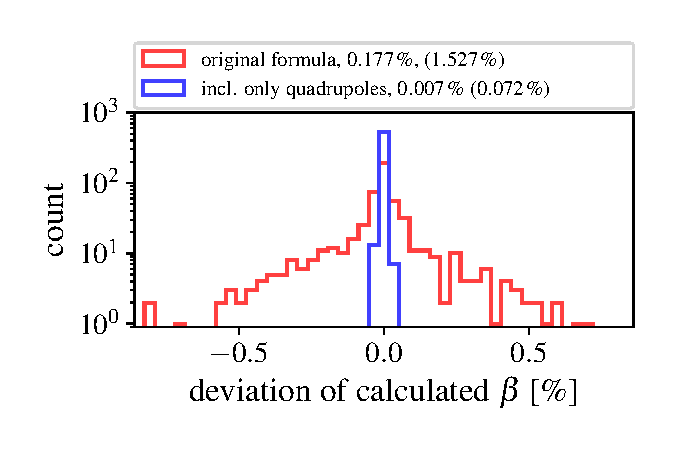
\includegraphics[width=.49\linewidth]{hist1518_ONLYQUADS_01}
  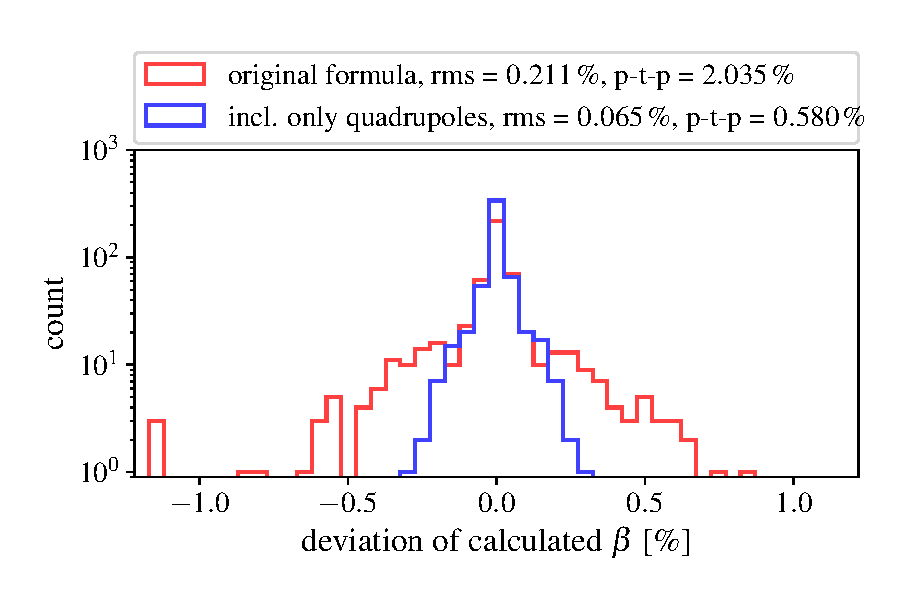
\includegraphics[width=.49\linewidth]{hist1518_NAIV_01}
	\caption{
        Left: Difference between the real (simulated) horizontal $\beta$-functions and the ones
        calculated by \eqref{eq_3bpm_method} in red and~(\ref{eq:18}) in blue, respectively. Data are from MADX
        simulations of a lattice with quadrupolar errors only.
        Right: The same quantities are evaluated for the case with additional magnet misalignments.
        the numbers which figure after the legend label show the root mean square of the deviation
        and the the peak-to-peak derivation in parenthesis.
    }
	\label{fig:hist1518}
\end{figure}
%
While the magnet misalignment errors can be approximated as \emph{effective} quadrupolar field errors
and integrated in \eqref{eq:h_ij} the BPM misalignments need a different approach as shown in the
next paragraph.

\subsection{Effect of transverse sextupole misalignments}

The magnetic field of a sextupole displaced horizontally by $ \Delta x $ reads
%
\begin{equation}
B_y = \frac{B}{2}((x + \Delta x)^2 - y^2)\quad .
\end{equation}
%
{This induces a quadrupolar field error whose strength $ \delta K_1 $ is}
%
\begin{equation}
\delta K_1 =  \left.\frac{1}{B_0\rho_0}\frac{\partial B_y}{\partial x}\right|_{x=y=0}
  = \frac{B}{B_0\rho_0}\Delta x \quad .
\end{equation}
%
This {term} can be used in \eqref{eq:h_ij} to include sextupole offsets in $ \bar{h}_{ij} $.

\subsection{Effect of longitudinal quadrupole misalignments}

%\begin{wrapfigure}{O}[\figborderhang]{8cm}
\begin{figure}
    \centering
    \includestandalone{quad_misal}
	\caption{
        The top sketch shows the displaced quadrupole (solid gray) relative to the original position
        (dashed). In the bottom sketch one can see the quadrupole at its original position with thin
        magnets on both ends.
    }
	\label{fig:quadmisal}
\end{figure}
%
The effect of a longitudinal displacement $ \delta s $ of a quadrupole magnet can be approximated by
leaving the magnet at its original position and introducing two thin magnets at its edges to mimic
the displacement, as shown in Figure~\ref{fig:quadmisal}.
The top part of the figure shows the actual situation:
The quadrupole is moved to the left such that it covers now the hatched area in addition to the gray
region. 
The bottom part illustrates the approximation method:
In the direction of the displacement there is an additional element with integrated field strength
$ \delta K_1 = k_1\delta s $ ($k_1$ being the 
non-integrated quadrupole strength), to simulate the part of the quadrupole that moved into this area
whereas an error 
$ -\delta K_1 $ is placed at the opposite end to compensate the part of the quadrupole that moved out
of this area.



\subsection{Effect of BPM misalignments}

An error, $ \delta s_i $, in the longitudinal position of
a BPM affects the evaluation of \eqref{eq:18} and \eqref{eq:h_ij} which rely on the model
values of $ \beta $ and $ \phi $ at the nominal position of the BPM.
Using \eqref{eq_phase} the phase error and the resulting $\beta$ shift at the position $s_i + \delta s_i$ can be approximated as
%
\begin{align}
\tilde{\phi}_i &\approx \phi_i + \frac{1}{\beta_i}\delta s_i\quad , 
\label{eq:Dphi} \\
\tilde{\beta}_i &\approx \beta_i + \frac{\partial \beta_i}{\partial s} \delta s_i  = \beta_i - 2\alpha_i \delta s_i \quad , \label{eq:Dbeta}
\end{align}
%
up to first order in $ \delta s_i $.

\subsection{Derivation of a corrected \texorpdfstring{$\beta$}{beta} from phase formula}

An equation similar to Eq.~(\ref{eq:18}) has to be re-derived by taking into account the considerations
of the preceding sections.

First, focusing errors, \eqref{eq_phasebeating_1st_app},
and BPM misalignments, \eqref{eq:Dphi}, are incorporated in the phase advance $\varphi_{ij}$:
%
\begin{align}
    \varphi^\text{err}_{ij}  &=
    \varphi_{ij}\m + \bar{h}_{ij} - 8\sin^2\varphi_{ij}\m\re{f_i} - 8 \sin\varphi_{ij}\m\cos\varphi_{ij}\m
    + \frac{1}{\beta_j\m}\delta s_j - \frac{1}{\beta_i\m}\delta s_i \notag \\
    &= \varphi_{ij}\m + \Delta\varphi_{ij}
    \fstop
    \label{eq_phi_err}
\end{align}
%
Together with the $\beta$~shift of \eqref{eq:Dbeta}, the $\beta$~beating \eqref{eq_betabeat} and the
$\alpha$~beating,
the quotient of the first row elements of the transfer matrix, \eqref{eq_trmat_quot}, reads
%
\begin{equation}
    \frac{
        \left(m_{ij}\right)_{11}
    }{
        \left(m_{ij}\right)_{12}
    }
    =
    \frac{1}{
        (\beta_i\m - 2\alpha_i\m\delta s_i)(1-8\im{f_i})} 
    \left(
        \cot \varphi_{ij}^\text{err} +  \alpha_i(1-8\im{f_i} -8\re{f_i}) \m
    \right)
    \fstop
    \label{eq_trmat_quot_gij}
\end{equation}
%
The cotangent above can be expanded in a Taylor series around $\varphi_{ij}\m$:
%
\begin{equation}
        \cot\varphi_{ij}^\text{err}
        =\cot\varphi_{ij}\m \left( 1 - 8\im{f_i}\right) + \frac{\bar{h}_{ij}}{\sin^2\varphi_{ij}\m} - 8 \re{f_i}
        + \frac{\frac{1}{\beta_i\m}\delta s_i + \frac{1}{\beta_j\m}\delta s_j}{\sin^2\varphi_{ij}\m}
\end{equation}
%
and \eqref{eq_trmat_quot_gij} can be simplified:
%
\begin{align}
    \frac{
        \left(m_{ij}\right)_{11}
    }{
        \left(m_{ij}\right)_{12}
    }
    =
    \frac{1}{\beta_i\m - 2\alpha_i\m\delta s_i} 
    \left(
        \cot \varphi_{ij}^\text{err} + \alpha_i \m + \bar{g}_{ij}
    \right)
\end{align}
%
with 
%
\begin{equation}
\bar{g}_{ij} = \text{sgn}(i-j)\dfrac{ \frac{1}{\beta\m(s_j)}\delta s_j - \frac{1}{\beta\m(s_i)}\delta s_i +
\sumw\beta_w\m\delta K_{w,1}\sin^2\phi_{wj}\m}{\sin^2\phi_{ij}\m}\quad ,
\label{eq:g_ij}
\end{equation}
%
To get the corrected $\beta$ from phase formula one has to follow the same steps as in section~\ref{sec_beta_meas}:
%
\begin{align}
    \frac{\left(m_{ij}\right)_{11}}{\left(m_{ij}\right)_{12}} - \frac{\left(m_{ik}\right)_{11}}{\left(m_{ik}\right)_{12}}
    =&
    \frac{1}{\beta_i} \left( \cot\varphi_{ij} - \cot\varphi_{ik}\right)
    %\notag \\
    -
    \frac{1}{\left(\beta_i\m - 2\alpha_i\m \right) } 
    \notag \\
    &\times\left[
        \cot\varphi_{ij}\m  + \bar{g}_{ij}
        -
        \cot\varphi_{ik}\m  - \bar{g}_{ik}
    \right]
\end{align}
%
and the final expression for the $\beta$~function at position $s_i$ from the combination $l$ reads
%
\begin{align}
\beta_l(s_i) \approx& \frac{\cot\phi_{i{j_l}} - \cot\phi_{i{k_l}}}{\cot\phi_{i{j_l}}\m - \cot\phi_{i{k_l}}\m +\bar{g}_{i{j_l}} - \bar{g}_{i{k_l}}} \left[\beta\m(s_i) - 2 \alpha\m(s_i) \delta s_i\right]
    \fstop
\label{eq:beta_g}
\end{align}
%
In order to account for sextupole misalignments and quadrupole longitudinal misalignments, it suffices
to add the corresponding effective $\delta K_1$ to the sum in $\bar{g}_{ij}$,
as described in the previous sections. 

Having defined the set I as
%
\begin{equation}
 I = \left[\min(i,j), \max(i,j)\right] \subset \mathbb{N}\quad ,
 \end{equation}
%
%\begin{wrapfigure}{O}[\figborderhang]{9cm}
\begin{figure}
	\centering
  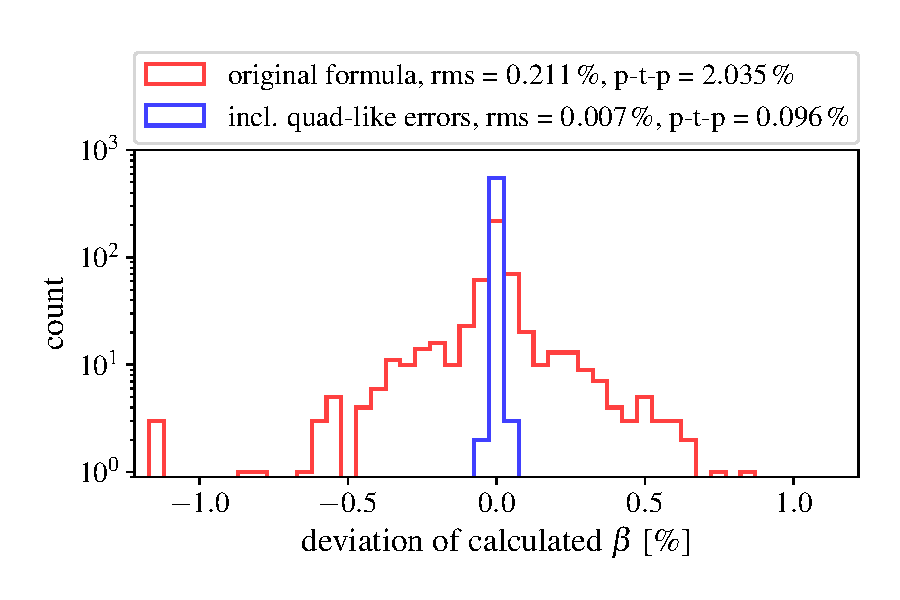
\includegraphics[width=.7\linewidth]{hist1518_EVERYTHING_01}
    \caption{Accuracy of the horizontal $\beta$-function evaluated via \eqref{eq_3bpm_method} and~\eqref{eq:beta_g} with the effect of magnets and BPM misalignments taken into account. The accuracy of
 \eqref{eq:beta_g} is similar to the one of \eqref{eq:18} with quadrupolar field errors only (Figure~\ref{fig:hist1518}).}
	\label{fig:hist1518_with_everything}
%\end{wrapfigure}
\end{figure}
%
so that an element with index $ w \in I$ lies between elements $ i $ and $ j $, \eqref{eq:beta_g}
and~\eqref{eq:g_ij} hold for every combination $ i $, $ j $, $ k $ of the BPMs.
 By doing so, we do not need to distinguish the three cases where the probed BPM is in the middle, left or right.


All these considerations can be put into \eqref{eq:beta_g} and used to get a more accurate
$ \beta $ function.
To verify the validity of \eqref{eq:beta_g}, its horizontal $\beta$-functions are compared to the
ones simulated by MADX along with the ones inferred from \eqref{eq_3bpm_method}, this time including
sextupole radial offsets and BPMs longitudinal shifts.

The result is shown in Figure~\ref{fig:hist1518_with_everything}. The accuracy is now as good as the one of \eqref{eq:18}  when only quadrupolar field errors were introduced in the
lattice, which in turn is much greater than the old formula, \eqref{eq_3bpm_method}.

\section{Calculation of the correlation matrix}
\label{sec_corr_matr}

The Jacobian $ \mathbf{T} $ of \eqref{eq:Tij} can be split into blocks 
%
\begin{equation}
\mathbf{T} = \left( \mathbf{T}^\phi \quad \mathbf{T}^K \quad \mathbf{T}^s\right),
\end{equation}
%
for the uncertainties of phase $ \mathbf{T}^\phi$, quadrupole field  $\mathbf{T}^K$ and BPM misalignment $\mathbf{T}^s$.
$ \mathbf{T}^\phi $ is the same of \eqref{eq:Tphiij}. For the quadrupolar field errors we get
%
\begin{align}
	T^K_{l\lambda}(s_i) = 
		\left. \frac{\partial \beta_l(s_i)}{\partial  K_{1,\lambda}}\right|_{\delta K = 0} =
		\mp\frac{\beta\m(s_i)\beta\m(s_\lambda)}{\cot\phi_{ij_l}\m - \cot\phi_{ik_l}\m}\left(
		\frac{\sin^2\phi_{\lambda j_l}\m}{\sin^2\phi_{ij_l}\m}A_{ij_l}(\lambda) - \frac{\sin^2\phi_{\lambda k_l}\m}{\sin^2\phi_{ik_l}\m}A_{jk_l}(\lambda)\right)\quad ,
\label{eq:TK}
\end{align}
%
  with 
%
\begin{equation}
    A_{ij}(\lambda) = \left\{\begin{array}{ll}
    1&\text{if }i<\lambda<j\\
    -1&\text{if }j<\lambda<i\\
    0&\text{else}
    \end{array}\right. \quad .
  \end{equation}
%
  The contribution from the BPM misalignment is calculated analogously:
%
\begin{align}
      T^s_{l\lambda}(s_i) &= \left.\frac{\partial \beta_l(s_i)}{\partial s_\lambda}\right|_{\delta s = 0} \notag \\
      &= -2\alpha^m(s_i)\delta_i^{\lambda}
      \mp 
      \frac{
          \dfrac{\text{sgn}(i-j_l)}{\sin^2 \phi_{ij_l}\m}\left(\dfrac{\beta\m(s_i)}{\beta\m(s_{j_l})}\delta^{j_l}_\lambda - \delta_\lambda^i\right) -
          \dfrac{\text{sgn}(i-k_l)}{\sin^2 \phi_{ik_l}\m}\left(\dfrac{\beta\m(s_i)}{\beta\m(s_{k_l})}\delta^{k_l}_\lambda - \delta_\lambda^i\right)}
      {\cot \phi_{ij_l}\m - \cot \phi_{ik_l}\m} \quad .
      \label{Ts}
  \end{align}
%
  In \eqref{eq:TK} and~\eqref{Ts} the minus and plus signs refer to the horizontal and vertical case, respectively. 
%In Equations~(\ref{eq:TK}) and~(\ref{Ts}) $\delta \epsilon = 0$ means \[\delta K_w = \delta s_w = \delta \phi_w = 0,\quad \forall w.\]

\section{Removal of bad BPM combinations}
\label{sec_bad_combs}


\begin{figure}
	\centering
    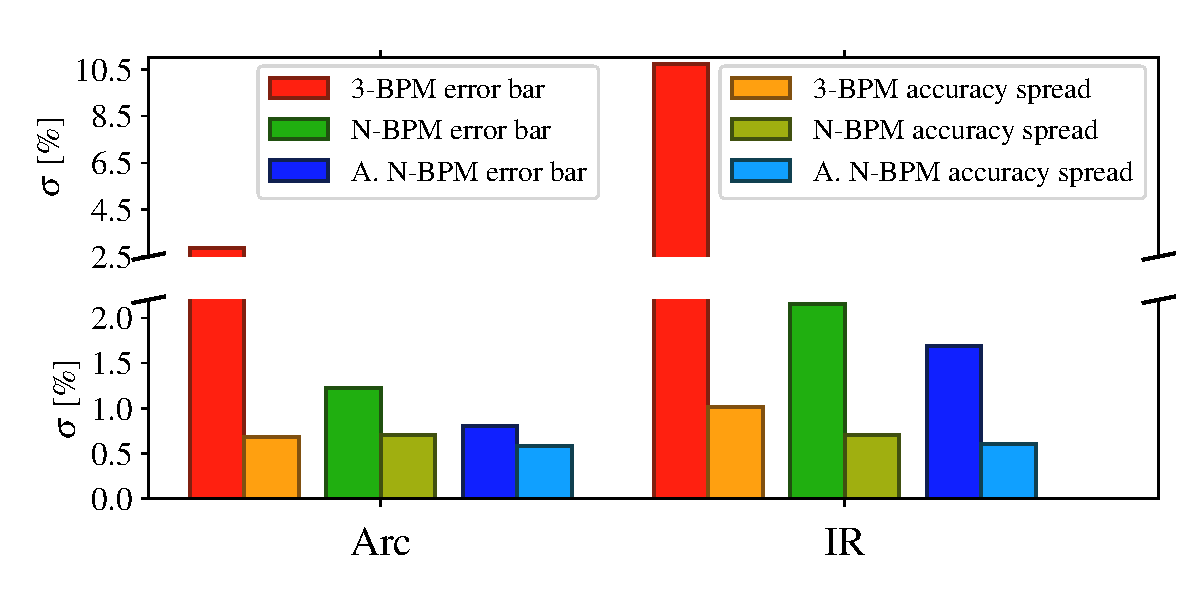
\includegraphics[width=.7\linewidth]{comparison_statistics_007_bars}
    \\
    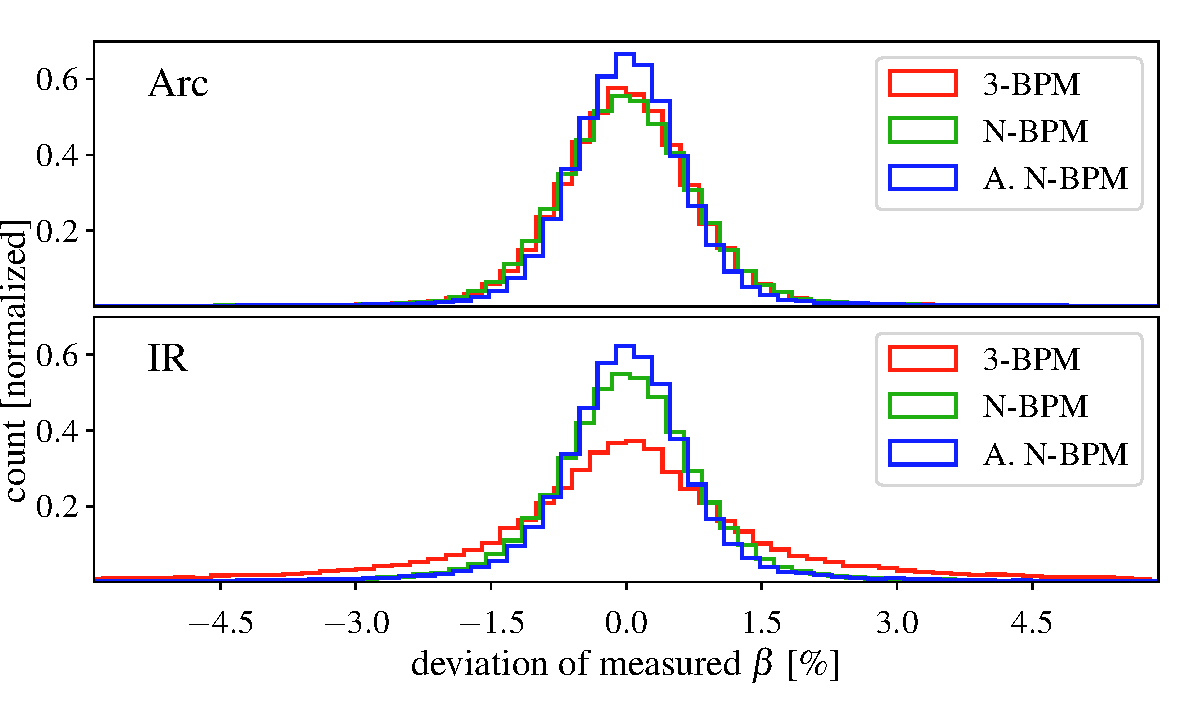
\includegraphics[width=.7\linewidth]{comparison_statistics_006}
	\caption{Comparison of the 3-BPM method, the original N-BPM method and the analytical N-BPM method (denoted as \texttt{A.N-BPM}) for the nominal LHC lattice at collision, with $ \beta^*=40\,\text{cm} $. BOTTOM: histogram of the difference to the real $\beta$-function in percent. TOP: the average of the error bars and the accuracy spread (width of a standard distribution fit to the distribution in the bottom plot) in percent.  The analytical N-BPM method has the best accuracy both in the arcs and in the IRs. Data have been cleaned of outliers.}
	\label{fig:compare_NBPM_to_3BPM}
\end{figure}
%
\begin{figure}
	\centering
    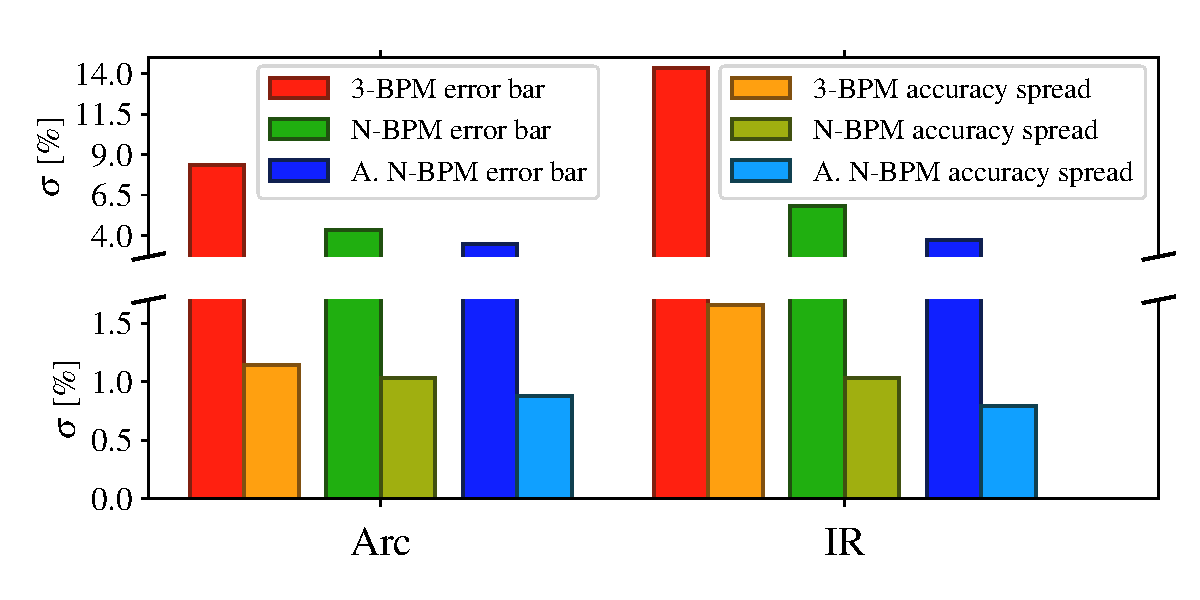
\includegraphics[width=.7\linewidth]{comparison_statistics_HL007_bars}
    \\
    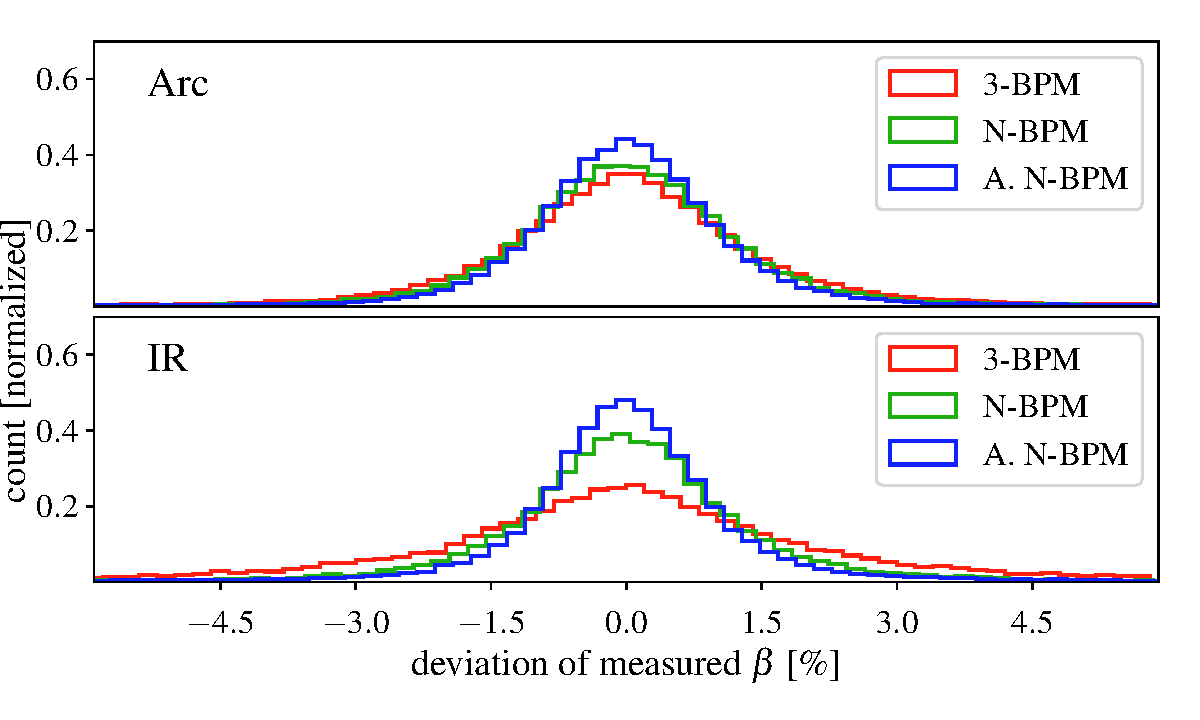
\includegraphics[width=.7\linewidth]{comparison_statistics_HL006}
	
	\caption{
        Same comparison of Figure~\ref{fig:compare_NBPM_to_3BPM} between the three methods for the
        HL-LHC $ \beta^*= 15\,\text{cm} $ ATS optics. The analytical N-BPM method yields clearly
        better results, both in the IRs and in the arcs. Compared to the $ \beta^*=40\,\text{cm} $
        optics shown in Figure~\ref{fig:compare_NBPM_to_3BPM}, the $ \beta $ function reconstruction
        is less accurate: This was also demonstrated for the $ \beta^*=20\,\text{cm} $ optics in
        \cite{LangnerNBPM}. }
	\label{fig:compare_ATS}
\end{figure}
%
\begin{figure}
	\centering
  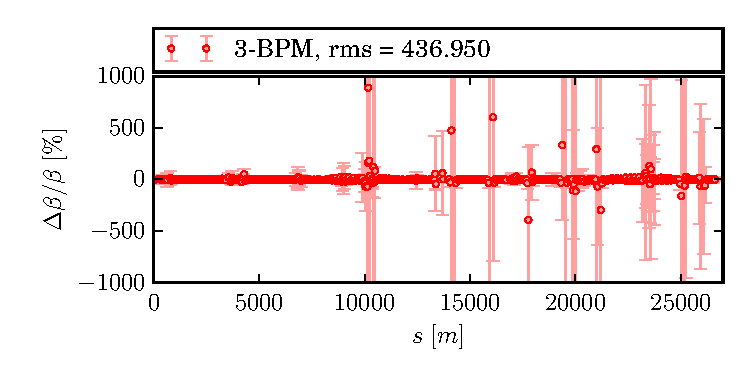
\includegraphics[width=.7\linewidth]{10cm_b1_x_3bpm}
    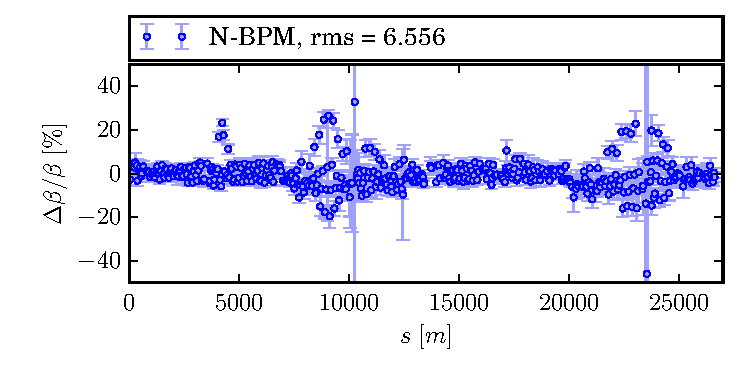
\includegraphics[width=.7\linewidth]{10cm_b1_x_nbpm}
	\caption{Horizontal $ \beta $ beating of beam 1 at $ \beta^*=10\,\text{cm} $ during the ATS MD 2016. TOP: 3-BPM method. BOTTOM: analytical N-BPM method. The 3-BPM method suffers from bad phase advances and has many outliers. The regions of high $ \beta $ beating at around $ \SI{8000}{m} $ and $ \SI{23000}{m} $ lie in the telescopic arcs. }
	\label{fig:10cm_beam1_hor_3bpm}
\end{figure}
%
\begin{figure}
	\centering
	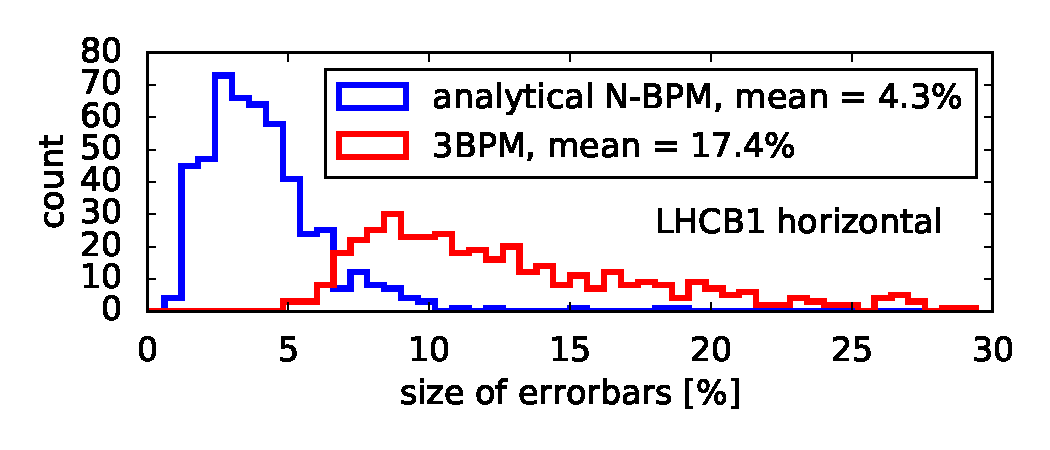
\includegraphics[width=.49\linewidth]{comparison_errorbars_Beam1}
	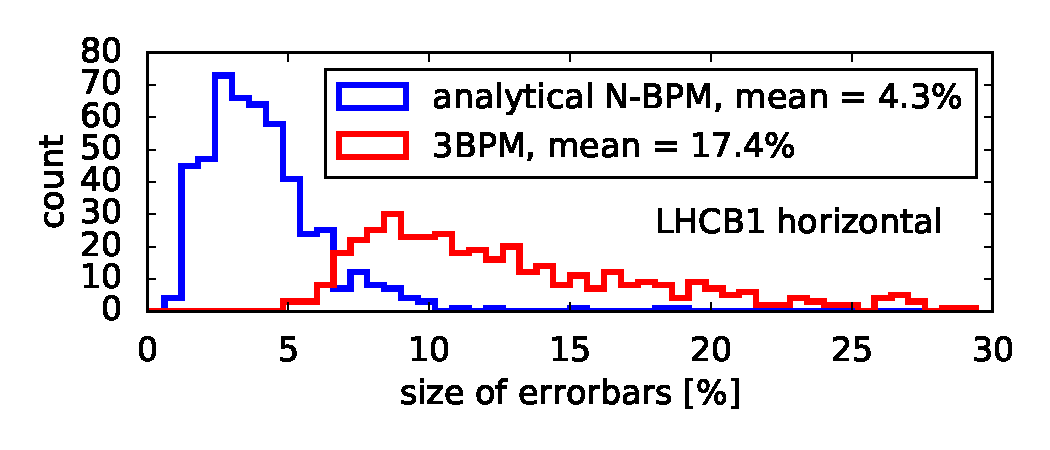
\includegraphics[width=.49\linewidth]{comparison_errorbars_Beam2}
	
	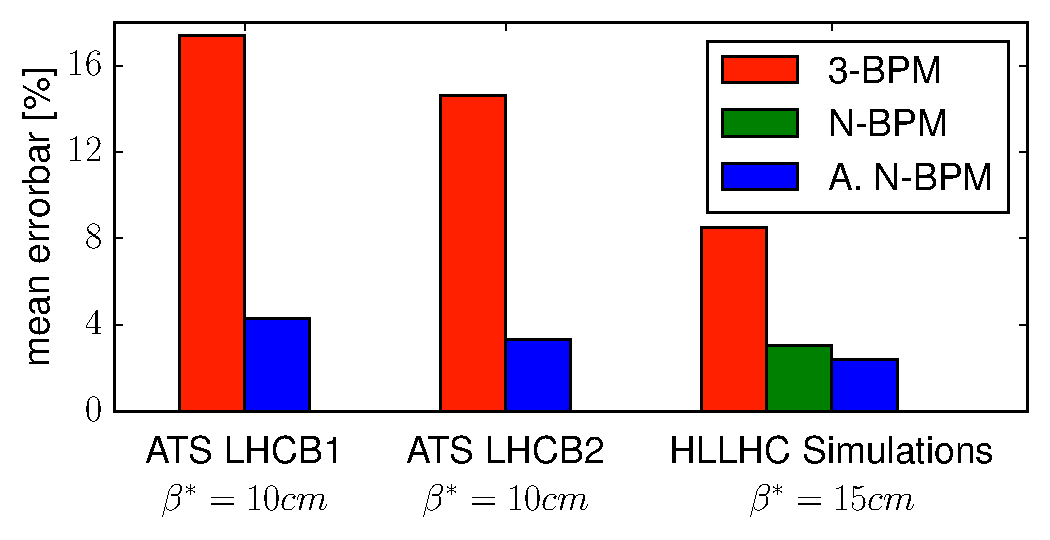
\includegraphics[width=.7\linewidth]{mean_errorbars}
	
	\caption{
        A comparison of the error bars of the $ \beta^*=10\,\text{cm} $ optics of the October 2016 MD.
        TOP: histogram of the errorbars of beam 1. CENTER: histogram of the errorbars of beam 2.
        BOTTOM: mean of the size the errorbars. The mean of the analytical N-BPM method is a factor
        4 more accurate than the 3 BPM method. The third set of values shows the mean of the errorbars
        of the simulations as shown in Figure~\ref{fig:compare_ATS} but for the whole ring.
        }
	\label{fig:HL_report/comparison_errorbars}
\end{figure}
%
Since a phase advance $ \phi_{ij} \approx n\pi $ results in an enhancement of phase measurement errors and in the extreme case numerically unstable values, a filtering was introduced. Instead of keeping a constant number of combinations as in \cite{LangnerNBPM} we set a threshold for \emph{bad} phase advances. A phase advance $ \Delta \phi $ is considered \emph{bad} if $ \Delta \phi \in [ n\pi - \delta, n\pi + \delta ] $ for $ n\in \mathbb{N} $ and a given threshold $ \delta $. If any of the four phase advances $ \phi_{ij_l}, \phi_{ik_l},\phi_{ij_l}\m,\phi_{ik_l}\m $ in Eq.~\eqref{eq_3bpm_method} is bad, the corresponding BPM combination is disregarded in the calculation of the weighted mean. This allows us to still use several combinations but skipping those which are numerically unstable. The current value for the threshold is $ \delta = 2\pi \cdot 10^{-2}$. The use of fewer combinations results in a lower computation time. 


To test the analytical N-BPM method and compare it to the original 3-BPM and the Monte Carlo N-BPM
method, a large set of LHC lattices with $ \beta^*=40\,\text{cm} $ with randomly distributed errors
is generated and a measurement is simulated by tracking a single particle via polymorphic tracking
code (PTC) \cite{Schmidt2002}. The random errors are created from table \ref{tab:unc_estimates}
and a Gaussian noise of $ \sigma_x = 0.1\,\text{mm} $ is applied to the BPM signal. No singular value
decomposition cleaning is applied since it would clean the artificial noise too efficiently
\cite{Langner2016}. The excitation amplitude is $\SI{0.8}{mm}$ at a $ \beta $ function of about
$ \SI{120}{m} $. The tracked particle positions are then analyzed by the three methods
(3-BPM, N-BPM and analytical N-BPM) and the respective deviation from the real horizontal
$ \beta $ function is shown in the bottom plot of Figure~\ref{fig:compare_NBPM_to_3BPM}.
The analytial N-BPM method includes the filtering of phase advances. Especially in the IR, where
neighbouring BPMs have often unsuitable phase advances, the N-BPM and analytical N-BPM method yield
more accurate values.

The top diagram of Figure~\ref{fig:compare_NBPM_to_3BPM} shows that the error of the 3-BPM method is considerable larger, whereas the N-BPM and analytical N-BPM method are very accurate with similar accuracies in the IR and arcs.


\section{HL-LHC}
\label{sec_hllhc_nbpm}
The ATS optics \cite{Fartoukh2013} is the baseline choice for the HL-LHC and our optics measurement
tools have to be prepared for the challenges imposed by such an optics. In Figure~\ref{fig:compare_ATS}
the three methods are compared in the same way as in Figure~\ref{fig:compare_NBPM_to_3BPM}.
The excitation amplitude was $ \SI{0.8}{mm} $ at a $ \beta $ function of $ \SI{127}{m} $.
For the current HL-LHC collision optics ($ \beta^* =15\,\text{cm}$) the performance of N-BPM and
analytical N-BPM method is again better than the 3-BPM method, especially in the IRs. All three
methods are, however, about a factor two more inaccurate than for the $ \beta^*=\SI{40}{cm} $ optics
of LHC, in agreement with Figure~7 of \cite{LangnerNBPM}.

In the post-processing of the data taken during the LHC Machine Development
measurement (MD) \cite{mdpubl} for testing the ATS principle with a $ \beta^* = 10$ cm optics, the analytical N-BPM method was used for the first time with filtering of bad phase advances. Figure 7 demonstrates that the analytical N-BPM
method deals well with the ATS MD optics. Monte Carlo simulations were
not possible for this optics.

Figure~\ref{fig:HL_report/comparison_errorbars} shows the precision of the final results for the $ \beta^*=10\,\text{cm} $ optics of both beams compared to the simulations of the HL-LHC lattice with $ \beta^*=\SI{15}{cm} $. To ease the comparison the errorbars are
shown in the bottom plot. They are slightly larger for the real measurement than those in simulations. We believe that the use of lower beam excitation   to ensure machine protection is behind these larger errorbars. Figure~\ref{fig:10cm_beam1_hor_3bpm} shows also that the 3-BPM method has many outliers and errorbars up to several kilometers caused by bad phase advances. Large error bars have been excluded for the mean shown in Figure~\ref{fig:HL_report/comparison_errorbars}.



The Monte Carlo simulations failed for low $ \beta^* $ optics and so we were not able to use the original N-BPM method during ATS MDs. This is another advantage of the analytical N-BPM method that it is
able to evaluate the systematic errors independently of the success of particle tracking.

\section{Conclusion}
\label{sec_nbpm_concl}

A new method for the measurement of beta and alfa functions has been
developed based on the existing N-BPM method.
A fully analytical calculation of the covariance matrix provides a faster and more accurate measurement
of $ \beta  $ and $ \alpha $ functions. The analytical N-BPM method also avoids the complications from
failing to find closed optics that occur in the Monte Carlo simulations  needed by the existing N-BPM method.
This stability with respect to the choice of optics model makes it more suitable for low $ \beta^* $ optics.
Simulations show that, together with a filtering of BPM combinations according to the phase advances,
the method is optimal for the HL-LHC upgrade. 

In the last years, the analytical N-BPM method has been used as standard method to measure the $\beta$~function in LHC
beam commissionning and machine development studies where it has been producing a high quality analysis
and contributed to the remarkable performance of the LHC in run~II.
The method also has been used in collaborative efforts
with accelerators from several external institutes like SuperKEKB (KEK) and PETRA~III (DESY). 


\chapter{A local observable for linear lattice imperfections}
\label{ch_localobs}

\newcommand{\combtoangle}[3]{
  $\SI{#1}{\degree} - \SI{#2}{\degree} - \SI{#3}{\degree}$
}

\newcommand{\noiserms}{$0.7\times 10^{-3}\times 2\pi$ rad{}}
\newcommand{\highnoise}{$1.8\times 10^{-3}\times 2\pi$ rad{}}

\newcommand{\maxfigwidth}{8.5cm}

\begin{chapterinfo}
  Finding a truly local observable for perturbations of the linear beam dynamics is a nontrivial task,
  contrary to the nonlinear regime, where local resonance driving terms already exist.
  The phase beating between two locations depends on errors outside of this region.
  However, phase advances between four nearby locations can be arranged in a way to cancel
  the contributions from errors outside of this region up to first order.
  The resulting local observable contains valuable information about quadrupolar lattice imperfections.
  This report seeks to explore this local phase beating observable and to test its usefulness
  for gaining insight in the linear optics imperfections of a circular accelerator. 

  This chapter is entirely based on original work of the author. Section~\ref{sec_lobster_intro}
  gives a brief introduction and motivation for the presented work. Section~\ref{sec:localobs} presents
  the main part with a rather technical derivation of the local observable.
  A thorough verification of the vailidity and possible use cases are presented
  in section~\ref{sec:robustness_check}, using the LHC as example.
  In section~\ref{sec:measurements} actual measurement data, acquired during LHC beam commissionning,
  conducted by the OMC team, is compared to the simulated results.  
  
The content of this chapter has been published in~\cite{Wegscheider2020}.
\end{chapterinfo}



\section{Introduction}
\label{sec_lobster_intro}

Special accelerator segments like the interaction regions of colliders
need a precise control of local optics which becomes a challenging task
if the optics are pushed to more extreme settings. New methods and more
precise hardware are required to measure and correct machine
imperfections such as quadrupole errors. In the case of a collider the
exact measurement and control of the $\beta$ function at the interaction point is important for operation of
the machine and to optimise luminosity~\cite{Coello2020}.

%For the correction of nonlinear lattice imperfections, resonance driving terms can successfully be
%used. This technique is performed successfully in the routine optics measurement and correction of
%LHC \cite{Persson2013}. \smallquest{are there others that use rdts?}

In order to locate error sources we are interested in local
observables, i.e. terms that only depend on lattice parameters and error sources in a localised
region. Such a local observable does not exist for linear lattice imperfections. For the non-linear
ones one has been found so far
\cite{Tomas2005, Franchi2007}: 
%
\begin{align}
  \chi(N) =& \frac{\hat{x}_1(N)}{\cos \left( \varphi_{x,12} - \frac{\pi}{2} \right)} 
  + \frac{\hat{x}_3(N)}{\cos\left( \varphi_{x,23}-\frac{\pi}{2} \right)} \notag \\
  &+ \hat{x}_2 (N) \left(
    \tan\left( \varphi_{x,12}-\frac{\pi}{2} \right)
    + \tan\left( \varphi_{x,23}-\frac{\pi}{2} \right)
  \right)
  \fstop
  \label{eq_chi}
\end{align}
%
$\chi (N)$ is built with the signal of three beam position monitors at positions $s_1, s_2, s_3$.

An extension of $\chi(N)$ into the linear regime does not seem possible since measured amplitude
and phase are used in a way to remove information on the linear beam dynamics.

Certain optics parameters (e.g. the $\beta$ function or coupling) can be calculated from the phase
advances between two or three BPMs \cite{Franchi2010, Miyamoto2010, Castro1996}
independently from BPM calibration errors \cite{Calaga2007}. 
The phase advance measured from a Fourier Transform \cite{Guo2016} turn-by-turn data is independent of the amplitude
of the signal and, thus, not affected by calibration errors.
%For coupling measurements, a reconstruction of the complex signal is necessary which requires using
%the amplitude \cite{Miyamoto2010}. The dependence on calibration can, in this case, be eliminated by using normalising
%the spectral lines by the main tune line.

%The $\beta$ function algorithms use only the phase advance which is independent of calibration errors
%whereas the coupling algorithm needs also the amplitude of the given spectral line. It is possible
%to remove the dependence on BPM calibration by taking the amplitude normalised to the main tune line.

The phase advance between two elements of an accelerator depends, in general, on all the elements in
the ring.
Focusing errors are of particular interest with their first order influence on the $\beta$~function.
The impact they cause on RDTs can be seen in \eqref{eq_f2000}, explicitly for a single error source
located at popsition $s_1$:
%
\begin{equation}
  f_{2000,j} = \delta K \beta_x(s_1) \e{2i\left[\varphi(s_j) - \varphi(s_1)\right]}
\end{equation}
%
%Therefore, all lattice imperfections in the machine alter the phase advance between two
%arbitrary positions.
\begin{figure}
  \centering
  \includestandalone[width=0.7\linewidth]{fig_local_error}
  \\[1.5em]
  \includestandalone[width=0.7\linewidth]{fig_local_error_inside}
  \caption{
    Sketch of the effect of a focus error $\Delta K$ on $f_{2000}$.
    The error creates a phase advance beating $\propto \e{2i\varphi\m}$.
    The incontinuity at the position of the source is caused by the propagation of the phase
    beating around the ring.
    TOP:
    If the error lies outside the interval from BPM1 to BPM2 and
    the model phase advance between the two BPMs is exactly $\pi$, the effect is the same and the
    phase advance beating is unaffected by this error.
    BOTTOM:
    If the error lies in between the two BPMs no cancellation is possible.
  }
  \label{fig_local_error}
\end{figure}
%
The top plot of Figure~\ref{fig_local_error} illustrates the effect of a single focusing error on the RDT.
In the case of a model phase advance of $\pi$ or a multiple of it, the effect is identical on both
BPMs, if the error does not occur in between them. In the other case both BPMs experience different effects
on their RDTs as shown in the bottom plot.

From \eqref{eq_tune_shift_quad} one can see that the effect on the phase advance depends,
up to first order, on global terms only in the form of $\re{f_j - f_i}$.


Under the assumption that coupling and higher order imperfections are negligible we
study the effect of quadrupolar field errors on the phase advance up to first order and construct an observable for
linear lattice imperfections that is local. For second order considerations we find a formula
for phase beating but global contributions cannot be eliminated.

The focus of this work lies on circular machines where phase advance can be measured accurately by
exciting an oscillation of the beam.
Excitation methods include single kicks and driven oscillation by an AC-dipole \cite{Miyamoto2008} which
generate a stable coherent motion of the beam.
Conceptually the local observable described in this work applies also to linear machines but accurate measurements
of phase advances remain challenging and the application of the proposed technique might not be practical.
Instead model-based fitting methods \cite{Zhang2018}
might be more suited to retrieve optics parameters directly.

%This article is organised in the following structure:
%
%Section \ref{sec:localobs} derives a local expression from the phase advance beating. This
%expression depends solely on the phase advances between four different BPMs.
%It reduces to just two BPMs if their mutual
%model phase advance is an exact multiple of $\pi$. 
%
%Section \ref{sec:robustness_check} examines the robustness of the local observable against noise and
%explores the visibility of strong error sources in the arc.
%
%Section \ref{sec:measurements} shows an example of a real LHC measurement of the local observable
%and the results are discussed.


% --------------------------------------------------------------------------------------------------
% ----- MAIN SECTION -------------------------------------------------------------------------------
% --------------------------------------------------------------------------------------------------

\section{Local observable}
\label{sec:localobs}


The effect of linear
lattice imperfections on the resonance driving terms (RDTs) and their impact on the betatron phase is
studied.
We express the betatron motion in the language of normal form and Courant-Snyder coordinates
\cite{Bartolini1997}.

The phase beating due to quadrupolar field errors is given by \eqref{eq_phasebeating_1st_app}
which is repeated here for convenience:
%
\begin{align}
  \Delta\varphi_{ij} = \bar{h}_{ij} - 8 \sin^2\varphi_{ij}\m\re{f_i} - 8\sin\varphi_{ij}\m \cos\varphi_{ij}\m\im{f_i} 
 +O(f^2)
\fstop
\label{eq_phasebeating_1st_app_again}
\end{align}
%
$\bar{h}_{ij}$ only depends on quadrupole errors inside the range $[i,j]$ and is therefore a local
term. The RDTs $f_i$ in \eqref{eq_phasebeating_1st_app}, on the other hand, contain global contributions.

The following subsections describe the derivation of an expression for local phase beating in two distinct
cases: The first is the general case with arbitrary phase advances between the BPMs. A combination of
four BPMs is necessary to calculate a pure local term. The second case considers only two BPMs with a
phase advance of $\pi$.

% --------------------------------------------------------------------------------------------------
\subsection{The general case -- phase advances different from \texorpdfstring{$n\pi$}{n*pi}}
\label{sec_generalcase}
%
\begin{figure}[htbp]
%\begin{wrapfigure}{O}[\figborderhang]{5cm}
  \centering
    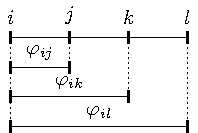
\includegraphics[width=.3\linewidth]{figIntervPhiIj}
  \caption{The interval of BPMs with corresponding phase advances.}
  \label{fig_interv_phi_ij}
%\end{wrapfigure}
\end{figure}
%
\equationref{eq_phasebeating_1st_app} still carries a dependence on the global error distribution in the form
of the terms $f_i$. We can eliminate those terms by carefully summing up phase advances between
different pairs of BPMs.


\label{sec_resummation}
The goal of this section is to eliminate global contributions to \eqref{eq_phasebeating_1st_app}.
This can be achieved a careful resummation of phase advances between four BPMs.

The global term $\re{f_i}$ can be eliminated by taking a third BPM $k$ and divide by the respective factor:
%
\begin{equation}
	\frac{\Delta\varphi_{ij}}{\sin^2\varphi_{ij}\m} - \frac{\Delta\varphi_{ik}}{\sin ^2\varphi_{ik}\m}
  =
	\frac{
    \bar{h}_{ij}
  }{
    \sin^2\varphi_{ij}\m
  } -
  \frac{
    \bar{h}_{ik }
  }{
    \sin^2\varphi_{ik}\m
  }
  - 8\left(\cot\varphi_{ij}\m - \cot\varphi_{ik}\m\right)\im{f_i}
    \fstop
    \label{eq_Deltaphi_first_step}
\end{equation}
%
Proceeding similarly with the factor in front of $\im{f_i}$:
%
\begin{equation}
  \frac{
    \frac{\Delta\varphi_{ij}}{\sin^2\varphi_{ij}\m} - \frac{\Delta\varphi_{ik}}{\sin ^2\varphi_{ik}\m}
  }{
    \cot\varphi_{ij}\m - \cot\varphi_{ik}\m } =
  \frac{
    \frac{ \bar{h}_{ij} }{ \sin^2\varphi_{ij}\m } -
    \frac{ \bar{h}_{ik } }{ \sin^2\varphi_{ik}\m }
  }{
    \cot\varphi_{ij}\m - \cot\varphi_{ik}\m
  }
  - 8\im{f_i}
    \fstop
    \label{eq_Deltaphi_second_step}
\end{equation}
%
We can simplify the lhs to:
{
\small
%
\begin{align}
  \frac{
    \frac{\Delta\varphi_{ij}}{\sin^2\varphi_{ij}\m} - \frac{\Delta\varphi_{ik}}{\sin ^2\varphi_{ik}\m}
  }{
  \cot\varphi_{ij}\m - \cot\varphi_{ik}\m }
  =&  \frac{\Delta\varphi_{ij}}{
    \sin^2\varphi_{ij}\m \left( \cot\varphi_{ij}\m - \cot\varphi_{ik}\m \right)
  }
  -
  \frac{\Delta\varphi_{ik}}{
    \sin^2\varphi_{ik}\m \left( \cot\varphi_{ij}\m - \cot\varphi_{ik}\m \right)
  } \notag \\
  =&
  \frac{
    \Delta\varphi_{ij}\sin\varphi_{ij}\m \sin\varphi_{ik}\m
  }{
    \sin^2\varphi_{ij}\m \left( \cos\varphi_{ij}\m \sin\varphi_{ik}\m - \cos\varphi_{ik}\m\sin\varphi_{ij}\m \right)
  }\notag \\
  &-
  \frac{
    \Delta\varphi_{ik}\sin\varphi_{ij}\m \sin\varphi_{ik}\m
  }{
    \sin^2\varphi_{ik}\m \left( \cos\varphi_{ij}\m \sin\varphi_{ik}\m - \cos\varphi_{ik}\m\sin\varphi_{ij}\m \right)
  } \notag  \\
  =& 
  \frac{
    \Delta\varphi_{ij}\left( 
    \sin \varphi_{ij}\m \cos \varphi_{jk}\m + \cos \varphi_{ij}\m \sin\varphi_{jk}\m\right)
  }{
    \sin\varphi_{ij}\m \sin \varphi_{jk}\m
  } \notag \\
  &-
  \frac{
    \Delta\varphi_{ik}\left( 
    \sin \varphi_{ik}\m \cos \varphi_{jk}\m - \cos \varphi_{ik}\m \sin\varphi_{jk}\m\right)
  }{
    \sin\varphi_{ik}\m \sin \varphi_{jk}\m
  } \notag \\
  =&
  \Delta\varphi_{ij} \left( 
    \cot \varphi_{ij}\m + \cot\varphi_{jk}\m
  \right)
  -
  \Delta\varphi_{jk} \left( 
    \cot\varphi_{jk}\m - \cot\varphi_{ik}\m
  \right)
  \fstop
\end{align}
%
}
The rhs of \eqref{eq_Deltaphi_second_step} can be simplified analogously and we can rewrite it to
%
\begin{align}
  & \Delta\varphi_{ij} \left( 
    \cot \varphi_{ij}\m + \cot\varphi_{jk}\m
  \right)
  -
  \Delta\varphi_{jk} \left( 
    \cot\varphi_{jk}\m - \cot\varphi_{ik}\m
  \right) \notag \\
  =& 
  \bar{h}_{ij} \left( 
    \cot \varphi_{ij}\m + \cot\varphi_{jk}\m
  \right)
  -
  \bar{h}_{jk} \left( 
    \cot\varphi_{jk}\m - \cot\varphi_{ik}\m
  \right)
  - \im{f_i}
  \fstop
  \label{eq_simplify_second_step}
\end{align}
%
To finally eliminate $\im{f_i}$ we take a fourth BPM, $l$, and subtract 
%
\begin{equation}
   \Delta\varphi_{ij} \left( 
    \cot \varphi_{ij}\m + \cot\varphi_{jl}\m
  \right)
  -
  \Delta\varphi_{jl} \left( 
    \cot\varphi_{jl}\m - \cot\varphi_{il}\m
  \right) \notag \\
  \label{eq_fourth_bpm}
\end{equation}
%
from \eqref{eq_simplify_second_step} and end up with
%
\begin{align}
 &\cot\varphi_{jl}\m \left( \Delta\varphi_{il} - \Delta\varphi_{ij} \right) 
 + \cot\varphi_{jk}\m \left( \Delta\varphi_{ij} - \Delta\varphi_{ik} \right) 
 - \cot\varphi_{ki}\m \Delta \varphi_{ik} + \cot\varphi_{li}\m\Delta\varphi_{il}\notag  \\
 =& 
 \cot\varphi_{jl}\m \left( \bar{h}_{il} - \bar{h}_{ij} \right) 
 + \cot\varphi_{jk}\m \left( \bar{h}_{ij} - \bar{h}_{ik} \right)
 - \cot\varphi_{ki}\m \Delta \varphi_{ik} + \cot\varphi_{li}\m\bar{h}_{il} 
\fstop
\label{eq_full_lhs_rhs}
\end{align}
%
Figure~\ref{fig_thetacomb} illustrates the collection of four BPMs used to construct
\eqref{eq_full_lhs_rhs}.
The left hand side of \eqref{eq_full_lhs_rhs} can be further simplified to
%
\begin{align}
 &\cot\varphi_{jl}\m \left( \Delta\varphi_{il} - \Delta\varphi_{ij} \right) 
 + \cot\varphi_{jk}\m \left( \Delta\varphi_{ij} - \Delta\varphi_{ik} \right) 
 - \cot\varphi_{ki}\m \Delta \varphi_{ik} + \cot\varphi_{li}\m\Delta\varphi_{il} \notag\\
 =&\cot\varphi_{jl}\m \Delta\varphi_{jl} - \cot\varphi_{jk}\m \Delta\varphi_{jk}
+ \cot\varphi_{ik}\m\Delta\varphi_{ik} - \cot\varphi_{il}\m\Delta\varphi_{il}
\fstop
  \end{align}
%
  Now we can rewrite \eqref{eq_full_lhs_rhs} as
%
\begin{equation}
  \Phi_{ijkl}^{\mathrm{meas}} = \Phi_{ijkl}^{\mathrm{model}} 
  \label{eq_Deltaphi_model_meas_app}
\end{equation}
%
by defining
%
\begin{align}
  \Phi^{\mathrm{meas}}_{ijkl} \equiv&
  \cot\varphi_{jl}\m\Delta\varphi_{jl} - \cot\varphi_{jk}\m\Delta\varphi_{jk}
  + \cot\varphi_{ik}\m\Delta\varphi_{ik} - \cot\varphi_{il}\m\Delta\varphi_{il} 
  \label{eq_deltaphi_firstorder_app}
\end{align}
%
and
%
\begin{align}
  \Phi_{ijkl}^\text{model} \equiv&
  \cot\varphi_{jl}\m\left(\bar{h}_{il} - \bar{h}_{ij}\right) 
  -\cot\varphi_{jk}\m\left( \bar{h}_{ij} - \bar{h}_{ik} \right)
  + \cot\varphi_{ik}\m \bar{h}_{ik} - \cot\varphi_{il}\m\bar{h}_{il}
  \fstop
  \label{eq_analyticalphi_firstorder_app}
\end{align}
%
Those terms are truly local to the region in between the four BPMs.


The resummation yields an observable
%
\begin{align}
  \Phi^{\mathrm{meas}}_{ijkl} =&
  \cot\varphi_{jl}\m\Delta\varphi_{jl} - \cot\varphi_{jk}\m\Delta\varphi_{jk} \notag \\
  &+ \cot\varphi_{ik}\m\Delta\varphi_{ik} - \cot\varphi_{il}\m\Delta\varphi_{il} 
  \label{eq_deltaphi_firstorder}
\end{align}
%
which only depends on measured phase advances between the four BPMs $i$, $j$, $k$ and $l$.
Up to first order it is equal to an analytic expression
%
\begin{align}
  \Phi_{ijkl}^\text{model} =&
  \cot\varphi_{jl}\m\left(\bar{h}_{il} - \bar{h}_{ij}\right) 
  -\cot\varphi_{jk}\m\left( \bar{h}_{ij} - \bar{h}_{ik} \right) \notag \\
  &+ \cot\varphi_{ik}\m \bar{h}_{ik} - \cot\varphi_{il}\m\bar{h}_{il}
  \label{eq_analyticalphi_firstorder}
\end{align}
%
which depends only on local error sources.
There are no global contributions left and the two quantities defined in Eqs. (\ref{eq_deltaphi_firstorder}) and 
(\ref{eq_analyticalphi_firstorder}) are truly local up to first order.
%
\begin{figure}
%\begin{wrapfigure}{O}[\figborderhang]{5cm}
  \centering
  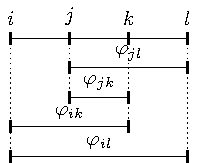
\includegraphics[width=.3\linewidth]{figThetaComb}
\caption{
  The phase advances appearing in Eqs.~(\ref{eq_deltaphi_firstorder}) and (\ref{eq_analyticalphi_firstorder}).
  The phase advances $\varphi_{ij}$ and $\varphi_{kl}$ do not appear in the final form of the local
  observable.
}
  \label{fig_thetacomb}
%\end{wrapfigure}
\end{figure}
%
The measurement uncertainty can be propagated to $\Phi_{ijkl}^\text{meas}$:
%
\begin{align}
  \sigma_\Phi^2 =& 
    \cot^2\varphi_{jl}\m \sigma_{\varphi_{jl}}^2
    + \cot^2\varphi_{jk}\m \sigma_{\varphi_{jk}}^2 \notag \\
    &+ \cot^2\varphi_{ik}\m \sigma_{\varphi_{ik}}^2 
    + \cot^2\varphi_{il}\m \sigma_{\varphi_{il}}^2
  \fstop
  \label{eq_Phi_err}
\end{align}
%
Equation~(\ref{eq_Phi_err}) is used to calculate the size of the errorbars in local observable plots.

A consideration of degrees of freedom suggests that three BPMs should suffice to reconstruct
the local linear optics errors. However, this reconstruction would depend on the amplitude which,
in turn, may suffer from calibration errors. The local observable presented here is independent of
BPM calibration errors.
%
\begin{figure}[h]
  \centering
  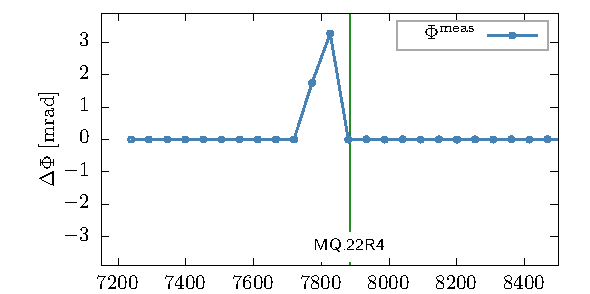
\includegraphics[width=.7\linewidth]{./sim_locality.pdf}
  \caption{The impact of a focusing error on the local observable. The plot shows an LHC arc with a
    relative error of $\SI{0.1}{\percent}$ of the magnetic field of focusing quadrupole \texttt{MQ.22R4}
    which is marked by a vertical line.
  }
  \label{fig_locality}
\end{figure}
%
Figure~\ref{fig_locality} illustrates the impact of a quadrupole error on the local observable.
The plot shows an LHC arc with $\SI{90}{\degree}$ FODO cells. Two BPMs are placed in one FODO cell, directly
in front of the focusing or defocusing quadrupoles, respectively.
The BPMS $i$, $j$, $k$ and $l$ are chosen to be consecutive ones.
A relative field error of $\SI{0.1}{\percent}$ was introduced at magnet \texttt{MQ.22R4}. Since the
points corresponding to a value of $\Phi_{ijkl}^\text{meas}$ are placed at the position $s_i$, only
the three points that precede the introduced error are affected, for which the introduced error lies
in the interval $[s_i, s_l]$.
The first of the three affected points has a very small value because of the proximity of the quadrupole
to the BPM.

\subsection{Exact multiples of \texorpdfstring{$\pi$}{pi}}

If the model phase advance is $\varphi_{ij}\m = n\pi$, the phase advance beating between two positions,
\eqref{eq_phasebeating_1st_app} reduces to
%
\begin{equation}
 % \phi_{ij}^\text{model} \equiv
  \Delta\varphi_{ij} = \bar{h}_{ij}
  \komma
  \label{eq_npi_localobs}
\end{equation}
%
which implies that $\Delta \varphi_{ij}$ is directly a local observable when
$\varphi_{ij}^\text{m}=n\pi$.
In this case the number of BPMs is reduced to two at positions $i$ and
$j$.
In general, phase advances that are sufficiently close to multiples of $\pi$ might not be present in
standard operation of an accelerator -- an exception is for example the ATS optics
\cite{Fartoukh2013} that is now used
in LHC and which is the proposed baseline for its high luminosity upgrade --, but it would be conceivable to prepare
special optics settings for a corresponding measurement in any acclerator.
The error of the local observable in this case,
%
\begin{equation}
    \sigma_{\Delta\varphi_{ij}} = \sigma_{\varphi_{ij}}
    \komma
    \label{eq_error_npi}
\end{equation}
%
is smaller than for the general local observable.

\subsection{Exploring the second order}
\label{ssec:second_order_phasebeating}

The details of the second order calculations can be found in the appendix. Here we summarise the results.
The detuning hamiltonian term $h_{1100,ij} $ as well as the RDT $f_{i} $ have to be extended to second order:
%
\begin{align}
  h_{1100,ij} &\rightarrow h_{1100,ij}^{(1)} + h_{1100,ij}^{(2)}\\
  f_{i} &\rightarrow f_{i}^{(1)} + f_{i}^{(2)}
  \fstop
  \label{eq_1st--2nd}
\end{align}
%
The total phase advance beating is, then,
%
\begin{align}
  \Delta\varphi_{ij} = &-2h_{1100,ij}^{(1)} 
  - 2h^{(2)}_{1100,ij}
  + 4\re{f_j^{(1)} - f_i^{(1)}} \notag\\
  &+ 4\re{f_j^{(2)} - f_i^{(2)}}\notag \\
  &+ 16 \left( \re{f_j^{(1)}} \im{f_j^{(1)}} - \re{f_i^{(1)}} \im{f_i^{(1)}} \right)\notag\\
  &+ O(K^{3})
  \fstop
  \label{eq_phadvbeating_2nd_inline}
\end{align}
%
The same resummation techniques as for the first order will not suffice to eliminate
global RDTs $f_i$ and $f_j$.
If we reformulate the third line of \eqref{eq_phadvbeating_2nd_inline} as
%
\begin{align}
   \re{f_j} \im{f_j} - \re{f_i} \im{f_i}  = 
   \frac{1}{2}\im{f_j^2} - \frac{1}{2}\im{f_i^2} \notag \\
    = \frac{1}{2} \im{ 
     A_{ij}^2 + 2A_{ij}f_i\e{2i\varphi_{ij}\m} + 
     \left( \e{4i\varphi_{ij}\m} - 1 \right) f_{i}^2}
  \label{eq_expanding2ndorder}
\end{align}
%
we see that it is not possible to separate the global $f_i$ from the local term $A_{ij}$. This
separation was the key to be able to eliminate the global terms in the first order approximation.

For $\varphi_{ij}\m = n\pi$ a second order term can be derived analogously:
%
\begin{align}
  \Delta\varphi_{ij} = & \bar{h}_{ij} - 2h_{1100,ij}^{(2)} \notag \\
  &+ 4\re{f_j^{(2)}-f_i^{(2)}} + 8\im{A_{ij}^{2}+ 2A_{ij}f_i}
  \fstop
  \label{eq_npi_second}
\end{align}
%
This term also contains the global $f_1$ and $f_2$ and there are no common factors that can be exploited
to eliminate them.

Therefore in this work purely local observable cannot be extracted from the second order phase beating.

% --------------------------------------------------------------------------------------------------
% ----- lobster ------------------------------------------------------------------------------------
% --------------------------------------------------------------------------------------------------

\section{Simulating Errors and Noise}
\label{sec_lobster}
\label{sec:robustness_check}

\subsection{General simulation setup}

In order to assess the usability of the local observable we perform a series of simulations with different
quadrupole error distributions and compare the prediction of the analytical calculations with simulated results. 
We base our simulations on the nominal LHC lattice at the end of run~II in 2018 with ATS optics and 
$\beta^*=\SI{30}{\centi\metre}$.

Figure~\ref{fig_combination} shows a sketch of a typical LHC arc section. BPMs are placed directly in
front of the quadrupoles of FODO cells. Additional trim quadrupoles (e.g. MQT) may be present.
%
\begin{figure}[htbp]
%\begin{wrapfigure}{O}[\figborderhang]{6cm}
  \centering
  \includestandalone[width=.7\linewidth]{figcombination}
  \caption{The probed interval $I_p$ for a typical section inside an LHC arc.
    BPMs are represented by rectangles.
    The phase advance between to consecutive BPMs is approximately $\SI{45}{^\circ}$.
    Used BPMs are shown in orange, unused in gray.
    Blue diamonds indicate quadrupoles and trim quadrupoles.
    Only BPMs and quadrupoles are shown, other elements such as corrector spool pieces and the
    bending dipoles are omitted.
  }
  \label{fig_combination}
\end{figure}
%
%\end{figure}
%
Four cases will be studied: the first one is a set of LHC design field
errors from WISE~\cite{wise1,wise2}, shown in Tab.~\ref{tab_design}, in the absence of phase noise.
This setup will let us verify the equality of Eqs.~(\ref{eq_deltaphi_firstorder}) and (\ref{eq_analyticalphi_firstorder}).
Then Gaussian noise of \noiserms{} is added to the simulated phase advances to illustrate the behaviour
in the presence of noise.
A third simulation includes an additional strong error source in one of the quadrupoles, c.f. Tab.~\ref{tab_design_peak}
to demonstrate the impact of single strong error sources and the locality of the local observable.
A last simulation setup demonstrates the visibility of quadrupolar errors originating from feed-down
of sextupoles via orbit offsets.

\begin{table}
  \begin{center}
    \begin{tabular*}{.5\textwidth}{l @ {\extracolsep{\fill}} c}
      Element & $\sigma_{K_1}/K\; [10^{-4}]$ \\
      MQ  & 12\\
      MQT & 75\\
      MQM & 12\\
      MQY & 11\\
      MQW & 15\\
      MQX & 1\\
      MB & 4\\
    \end{tabular*} \\
    \caption{Error distribution for the design LHC lattice at $\SI{6.5}{TeV}$ with weak errors in the final triplet in
      order to avoid higher order effects.
      $K$ denotes the main field component (quadrupolar field for quadrupoles, etc).
    }
   \label{tab_design}
  \end{center}
\end{table}

\begin{table}
  \begin{center}
    \begin{tabular*}{.5\textwidth}{l @ {\extracolsep{\fill}} c c}
      Element & $\delta K_1/K\; [10^{-4}]$ & $\sigma_{K_1}/K\; [10^{-4}]$ \\
      MQ.22R4.B1 & 100 & -\\
      MQ  & - & 12\\
      MQT & - & 75\\
      MQM & - & 12\\
      MQY & - & 11\\
      MQW & - & 15\\
      MQX & - & 1\\
      MB &-& 4 \\
    \end{tabular*}
    \caption{
      In addition to design LHC errors distribution we introduced a single strong error source in
      arc45.
    }
    \label{tab_design_peak}
  \end{center}
\end{table}

There are many different possible combinations of BPMs. In the following comparison plots we will only show
two of them: one that has a phase advance of $\SI{180}{\degree}$ in one of the phase advances appearing in
Fig.~\ref{fig_thetacomb_ij-kl} and one that avoids such a term and,
additionally, the 2-BPM combination with $\varphi_{ij}=\SI{180}{\degree}$.

In a real measurement we would consider only the combinations of closest BPMs to avoid the
accumulation of systematic errors coming from other lattice elements and therefore we limit our study
to only those combinations.
The phase advance over two FODO cells in telescopic arcs of the ATS optics is tightly matched
to $\pi$. On the one hand this provides a continuous set of combinations with
similar phase advances and thus we can more easily compare the values of $\Phi_{ijkl}^\text{model}$
and $\Phi_{ijkl}^\text{meas}$ at different positions.
On the other hand this gives rise to model phase advances close to multiples of $\pi$ for several
combinations which gives the possibility to explore these cases.
Table~\ref{tab_combs} shows the closest combinations with all occuring model phase advances.
Reflected combinations are omitted. Model phase advances close to $n\pi $ cause the cotangent
terms to diverge. They are therefore highlighted in red.
Since we still want to study these cases and avoid divergences and the resulting numerical instabilies
we impose a filter on the phase advances. 
Those which are closer to $n\pi$ than $10^{-6}\times 2\pi$ are excluded. 
The case \combtoangle{45}{90}{45} is sketched in Fig.~\ref{fig_thetacomb_ij-kl}.
%
\begin{figure}
  \centering
  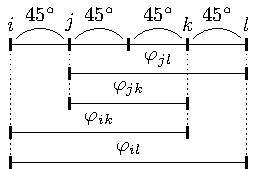
\includegraphics[width=.4\linewidth]{figThetacombijkl}
  \caption{The phase advances of the combination
    $\varphi_{ij}=\SI{45}{\degree}$, $\varphi_{jk}=\SI{90}{\degree}$, $ \varphi_{kl}=\SI{45}{\degree}$.
The phase advance $\varphi_{il} = \SI{180}{\degree}$ causes $\cot\varphi_{jl}\m$ to diverge.
  }
  \label{fig_thetacomb_ij-kl}
\end{figure}
%
%$cot n\pi = \infty$ for $n \in \mathbb{Z} $, so 

\begin{table}[htbp]
    \begin{center}
    % #publish_picture figTable1
    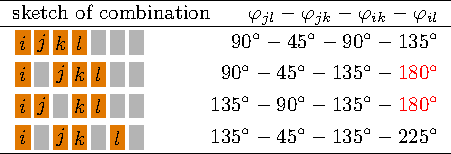
\includegraphics{figTable1}
    \end{center}
    % #end publish_picture
    \caption{Indices $i,j,k,l$ and phases appearing model phase advances for the closest combinations.
      The actual model phase advances depend on the respective model settings and differ slightly from
      the exact values above.
    }
    \label{tab_combs}
\end{table}

Model and measurement values are shown for the combinations \combtoangle{45}{45}{45} and
\combtoangle{90}{45}{45} and $\varphi_{ij}\m = \SI{180}{^\circ}$ in Figures~\ref{fig_design_nonoise}~to~\ref{fig_peak_noise}.
Since we get the phase advances of Table~\ref{tab_combs} only for telescopic arcs and for the sake
of readability we limit the plot region to just one telescopic arc, the one between IR4 and IR5.
For simplicity we show only results for the horizontal plane. 


\subsection{Design field errors}

The first case, Fig.~\ref{fig_design_nonoise}, is free of noise with the quad error distribution of
Tab.~\ref{tab_design}.
The agreement between analytical and measurement values is excellent, showing the validity of
Eqs.~(\ref{eq_deltaphi_firstorder}), (\ref{eq_analyticalphi_firstorder}) and (\ref{eq_npi_localobs}).

\newcommand{\errdist}{design}
%
\begin{figure}
  \centering
  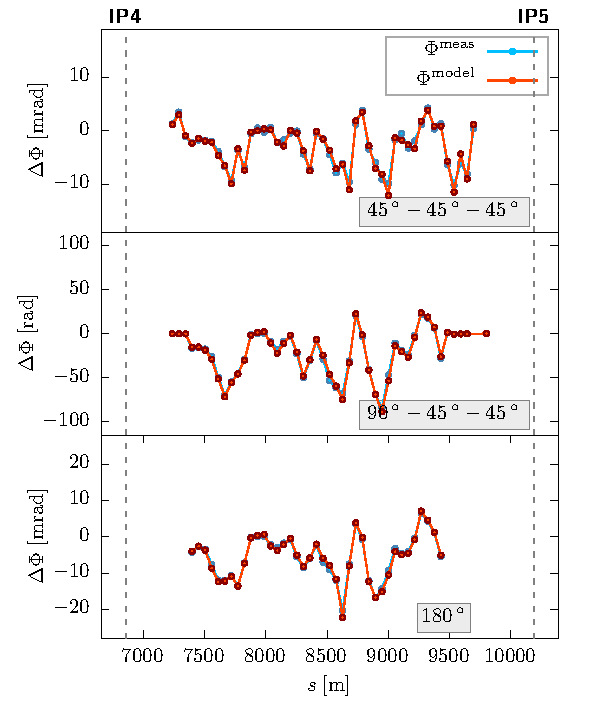
\includegraphics[width=.8\linewidth]{sim_no_noise}
  %\includegraphics[width=\linewidth]{./73_plots/sim_ij-kl_design_IP4}
  \caption{
    This figure shows the first two combinations of Tab.~\ref{tab_combs} and the case $\varphi_{ij}\m = \pi$
    from simulations.
    Top: the combination \combtoangle{45}{45}{45}.
    Center: the combination $\SI{90}{\degree}-\SI{45}{\degree}-\SI{45}{\degree}$. The absolute value of the local observable in the telescopic arc
    (right of IP4) is four orders of magnitude higher than in the top plot.
    The plots only show values where the phase advances do not differ more than $\SI{1}{\degree}$
    from the target values displayed in Tab.~\ref{tab_combs} in order to ensure comparability between
    the values. Additionally values with a model phase advance in $n\pi \pm 10^{-6}$ are excluded
    to avoid numerical instabilities.
    This causes the IR to be empty of local phase advances. 
    Note that in the middle plot the values are four orders of magnitude higher than in the other two.
    This originates from the $\cot\varphi_{il}\m$ terms which are high because of $\varphi_{il}\m \approx \pi$.%Values in non-telescopic arcs are strongly suppressed.
    The bottom plot shows the local observable for model phase advances of $\SI{180}{^\circ}$. 
    In all three plots the agreement between model and simulation is excellent.
  }
  \label{fig_design_nonoise}
\end{figure}
%
To examine the behaviour of the local observable in the vicinity of $n\pi$ we have to scan the accelerator
for available model phase advances. For each BPM $i$ we are looking for a second one -- BPM $j$ -- that
is placed at $\Delta\varphi_{ij} = \pi\pm\delta\phi$ downstream.
$\delta\phi$ is a threshold parameter controlling how many local observable pairs are accepted.
We chose $\delta\phi=\SI{1e-3}{}\times2\pi$.
The telescopic arcs of the ATS optics provide the needed model phase advances.

The agreement is, as for the general case, very good in the absence of errors.

\subsection{Phase noise}

The noise to signal ratio decreases with increasing oscillation amplitude and thus with increasing
$\beta$ function at the BPM. In the LHC FODO cells BPMs are installed close to the focusing and
defocusing quadrupoles and those lie at $\beta$ function maxima and minima, respectively.
Therefore we can divide the arc BPMs in two categories, those with low $\beta$ function and those with
high $\beta$ function. The $\beta$ function minima are usually around $\SI{30}{\meter}$ and the
maxima at $\SI{180}{\meter}$.
The phase advance uncertainties $\sigma_{\varphi_{ij}}$ fall into three categories:
both BPMs have high $\beta$ function, only one of them has high $\beta$ and both have low $\beta$.

For this set of simulations we introduce phase noise which
corresponds to noise values of the LHC signal that we typically achieve taking five data acquisitions
and after cleaning \cite{Calaga2004} and harmonic analysis.
We group BPMs into the before mentionned categories and apply a Gaussian error distribution
to the phase values according to measurement statistics.

With the introduced phase noise the agreement decreases significantly (cf. Fig.~\ref{fig_design_noise}). The noise is of the same order of magnitude
as $\Phi_{ijkl}^\text{meas}$ itself.
Therefore the LHC arc quadrupolar errors cannot be identified with this phase advance resolution.
The combination \combtoangle{45}{45}{45} shows the worst behaviour under noise because the $\beta$
function alternates between high and low values from BPM to BPM and so within the four neighbouring
BPMs there are always two with low $\beta$ function.
%
\begin{figure}
  \centering
  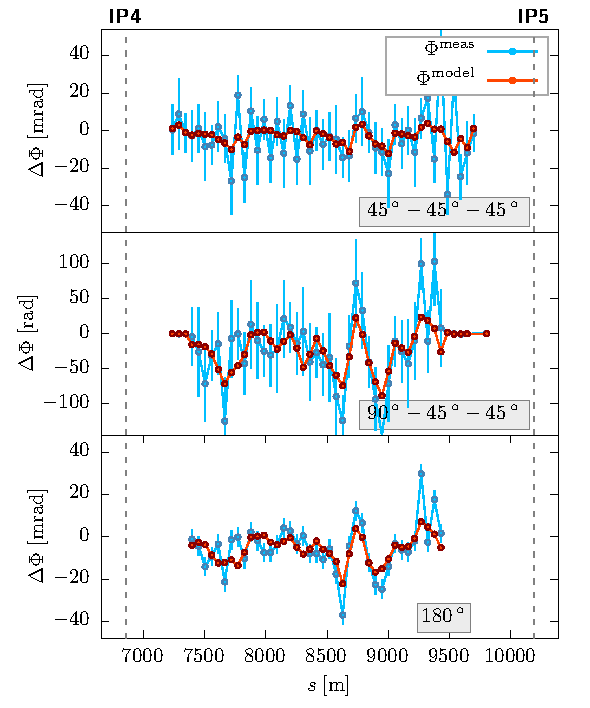
\includegraphics[width=.8\linewidth]{sim_noise} %\includegraphics[width=\linewidth]{./73_plots/sim_ij-kl_design_IP4_noise}
  \caption{
    Similar plots as in Fig.~\ref{fig_design_nonoise} but including a phase error of \noiserms{} for
    high $\beta$ function values and \highnoise{} for low $\beta$s.
    The agreement between model and simulation and measurement is highly deteriorated.
    The error bars have been calculated using Eqs. (\ref{eq_Phi_err}) and (\ref{eq_error_npi}).
    The case $\varphi_{ij}\m=\pi$ is affected less by the error since only one phase advance error
    is propagated.
  }
  \label{fig_design_noise}
\end{figure}
%
The case of exact $\pi$ phase advances shows the smallest errors as only one phase advance
error enters in the error propagation.

\subsection{Single strong error source}

For the next simulation, we assume that there is a single strong error in one of the quadrupoles. We
assign $1\%$ of relative error to MQ.22R4 to show the effect of a strong error source. Figure~\ref{fig_peak_noise}
shows that this error creates a visible peak in the local observable.
The peak in the local observable is situated immidiately in front of the location of the error source
because the plot shows the local observable at the position of BPM $i$ but the errors of the interval
$(s_i, s_l)$ enter in the calculation of the observable.

In the presence of model phase advances close to $n\pi$ the values of the local observable in the
telescopic arcs are clearly enhanced (c.f. bottom plot of Fig.~\ref{fig_design_nonoise} and
Fig.~\ref{fig_design_noise}).

The simulations above show that strong quadrupolar error sources ($\geq 1\%$) can be detected with the local
observables under the studied phase resolution.
For the detection of smaller errors a higher precision of the phase measurement would be needed.
More precise BPMs like DOROS-BPMs \cite{Gasior2011} currently installed in the LHC interaction region and a higher excitation
amplitude as well as the acquisition of a higher number of turns
can increase the resolution of the phase measurement. 
%
\begin{figure}
  \centering
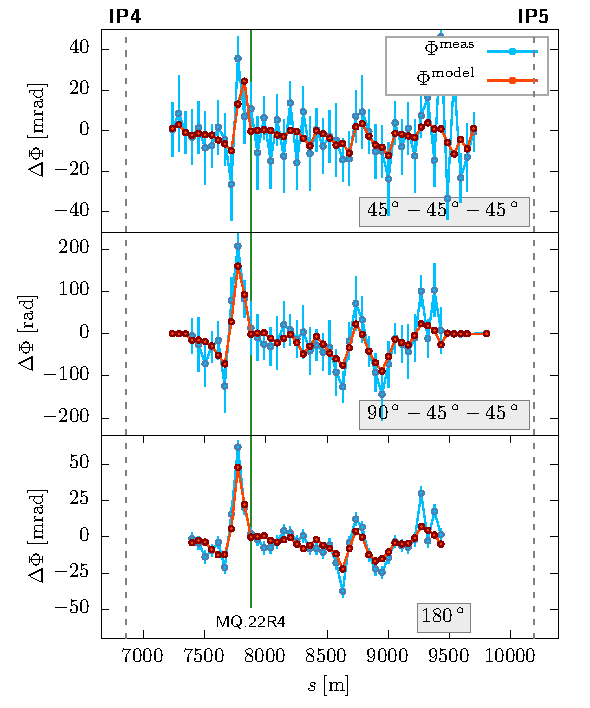
\includegraphics[width=.8\linewidth]{sim_peak}
\caption{The local observable with the error distribution of Tab.~\ref{tab_design_peak}, including
    a strong error source at \texttt{MQ.22R4.B1} and phase
    noise of \noiserms.
    %The combination \combtoangle{90}{45}{45} is less affected by the phase noise.
    The position of the strong error source is marked by a green line.
  }
  \label{fig_peak_noise}
\end{figure}
%
\subsection{Feed-down from sextupoles}

As final test case we introduce orbit offset into the machine around the IPs by activating dedicated dispersion
bumps. These are used in the ATS optics to compensate dispersion created by the crossing angles at the IPs.
The transverse displacement of the beam creates quadrupolar-like errors inside sextupoles via feed-down:
%
\begin{equation}
  \Delta K_{1,\text{sext}} = \delta x K_2
  \label{eq_sext_fedddown}
\end{equation}
%
where $\delta x$ denotes horizontal offset and $K_2$ is the strength of the sextupole. $K_{1,\text{sext}}$
can now be used for the calculation of the local observable.



Figure~\ref{fig_disp_noise} shows the local observable in this case. Regular bumps created by the
feed-down appear which are consistent in all three cases but less pronounced in the nearest neighbors case.
With the given noise level those bumps can be measured.
The local observable is not affected by feed-down in the center of the arc because sextupoles at places
with high orbit offset are turned off.
In comparison to the previous examples, Figs.~\ref{fig_design_noise} and \ref{fig_peak_noise}, the
values of the local observable did not change in this region.

The bottom plot of Fig.~\ref{fig_disp_noise} shows the changed orbit for reference.
The peaks of the local observable can be identified with the peaks in the orbit.
Again the local observable is in 
advance of the error source.
%
\begin{figure}[t]
  \centering
  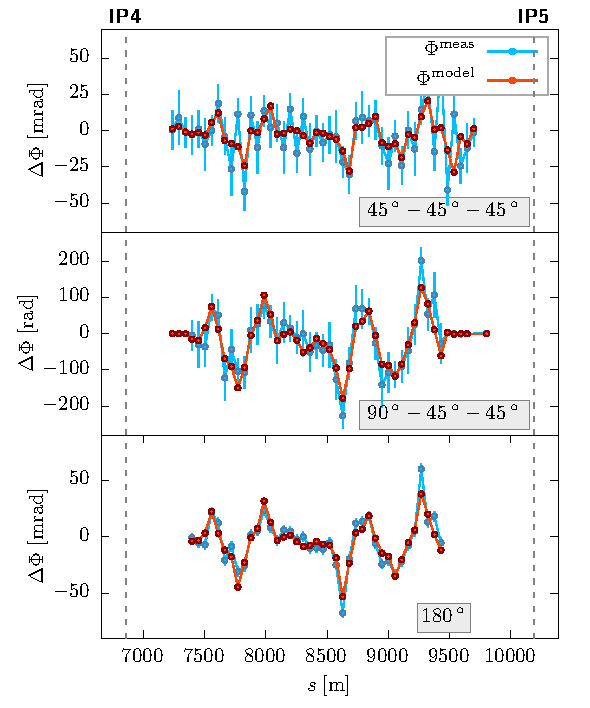
\includegraphics[width=.8\linewidth]{sim_disp}\\
  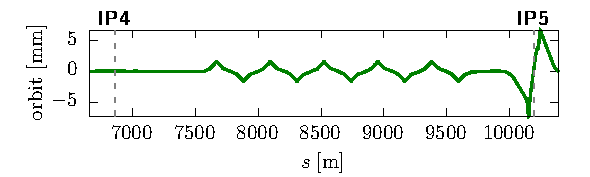
\includegraphics[width=.8\linewidth]{sim_orbit_x_noise_disp}
  \caption{The local observable with the error distribution of Tab.~\ref{tab_design} and phase noise
    of \noiserms. Additionally the orbit has been changed by dispersion bumps. The orbit offset creates
  feed-down from sextupoles.}
  \label{fig_disp_noise}
\end{figure}
%
\section{Experimental verification}
\label{sec:measurements}

\begin{figure}[t]
  \centering
  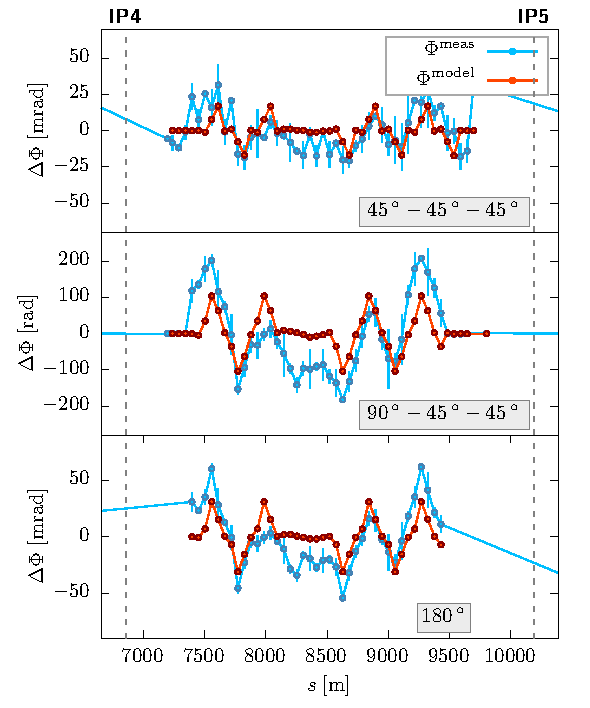
\includegraphics[width=.8\linewidth]{meas}
  %\includegraphics[width=\linewidth]{best_design_errors_meas_--l__ij-kl---}
  \caption{Plot of measurement data of the LHC commissionning 2018 at $\beta^*=\SI{30}{\centi\metre}$.
    The errorbars include statistical errors
    obtained from the phase measurement of the FFT.
    The effect of dispersion bumps on the local observable is clearly visible and matches well the
    prediction. The center region shows only a small effect from sextupoles.
  }
  \label{fig_measlobster002}
\end{figure}
%
We calculate the local observable from a measurement taken during the LHC beam commissionning in 2018.

The measurement can be seen in Fig.~\ref{fig_measlobster002} for the combinations \combtoangle{45}{45}{45}
(top plot) and \combtoangle{90}{45}{45} (bottom plot).

We take a model lattice where dispersion bumps are turned off in order to see the impact on the 
local observable.
As discussed in section~\ref{sec_lobster}, the feed-down of sextupole fields due to the orbit offset
of those bumps changes the local observable.
Figure~\ref{fig_measlobster002} shows in blue the measured local observable which features similar
spikes as the simulation (cf. Fig.~\ref{fig_disp_noise}).
In red the effect of feed-down from sextupoles via the orbit offset on the local observable is shown.
The feed down has been calculated by introducing the dispersion bump knob into the model that was turned
on during the measurement and calculating $\delta K_{1, \text{sext}}$ from \eqref{eq_sext_fedddown}.
The pattern of the model
values is also present in the measurement which confirms that their origin is indeed the feed-down.
Since the $\Phi_{ijkl}^\text{model}$ contains only the expected feed-down from sextupoles and no other
error sources (like normal quadrupole imperfections) the difference between model and measurement is
then the actual local observable created by those error sources.
The center region of the arc is free of a high peak because, as in the simulation, no sextupole is 
active at high orbit offsets.

\section{Conclusion and Outlook}

We showed the existence of a local observable for linear lattice imperfections in circular
accelerators. The locality of the observable holds up to first order in the quadrupole error
$\delta K_1$. 

Phase measurement noise is an issue with the current precision of turn-by-turn measurements and a
higher resolution in the measurement would be of advantage. For certain use cases, new techniques are
needed to improve the control of the machine and hardware upgrades are a justified solution.
Simulations show that strong error sources can be identified even with current precision of LHC measurements
as they generate distinguishable peaks.

The calculated local observable of an actual measurement shows a picture that is compatible with simulations.
Feed-down of orbit offsets via sextupoles can be seen in measurement data and be reproduced in simulations.

A future application of the observable to find strong local sources and to guide local error corrections
is foreseen for run~III of the LHC.


\chapter{Advanced transverse coupling measurement} 
 \label{sec_coupling}

\begin{chapterinfo}
    The compensation of the driven motion is necessary for a reliable coupling measurement.
    This chapter introduces methods to compensate for driven beam motion in the calculation of
    coupling resonance driving terms. The methods currently applied in the LHC are revised and
    recent findings are presented.
\end{chapterinfo}

\section{Driven coupled motion}
 In the past two methods were used for coupling measurements in
the LHC, the first one uses only the difference in tunes to rescale the coupling terms, this is
a naive approach because it disregards the driven betatron phase but often this approximation is
good enough to get a first estimate of the coupling in the machine. We refer to this method as the
\emph{model method}.

The second method \cite{Miyamoto2010} applies a detailled study of the driven particle motion and
provides a compensation for all optics parameters that enter into the coupling terms. This method will
be called \emph{formula method} in the following.

Recent findings \cite{Carlier2020} show that the AC-dipole locally effects RDTs and introduces
a jump at its location. The detailled considerations of the formula method lack such an effect.
In view of the suggestions of \cite{Carlier2020} this work presents calculations of the terms
$f_{1001}$ and $f_{1010}$, building upon the techniques introduced in \ref{sec_driven_coords}.
A comparison between model method, formula method and the newly calculated coupling terms are shown.


\subsection{AC-dipole as skew quadrupole}

To start the section about the beam motion that is driven \emph{and} coupled, we state a curious
analogy between AC-dipole and skew quadrupoles.

Throughout this chapter we use the following convention:
%
\begin{align}
    f_+ &\equiv f_{0101} \text{ and}\notag \\
    f_- &\equiv f_{0110} 
    \fstop
\end{align}
%
The RDTs in \eqref{eq_f0101_f0110} can be reformulated:
%
\begin{equation}
    f_\pm = 
    \frac{
        \sum\limits_w J_{1,w} \sqrt{\beta_{x,w}\beta_{y,w}}
        \e{
            i\left[\varphi_{wj,x} \pm \varphi_{wj,y}\right]
            -i\pi\left[Q_x\pm Q_y\right]
        }
    }{
        8i\sin[\pi(Q_x\pm Q_y)]
    }
    \fstop
\end{equation}
%
The coupled motion for a single coupling source now reads
%
\begin{align}
    h_x(s_j,N) =& \zxp(s_j,N) \notag \\
    &+2i\frac{
         J_{1,w} \sqrt{\beta_{x,w}\beta_{y,w}}
    }{
        8i\sin[\pi(Q_x + Q_y)]
    }
    \zyp(s_j,N)
        \e{
            i\left[\Delta\phi_x^+ + 2\pi Q_x \Theta(s_j,s_w) + 2\pi Q_y \Theta(s_j,s_w)\right]
            -i\pi\left[Q_x + Q_y\right]
        }
        \notag \\
    &+2i\frac{
         J_{1,w} \sqrt{\beta_{x,w}\beta_{y,w}}
    }{
        8i\sin[\pi(Q_x - Q_y)]
    }
    \zym(s_j,N)
        \e{
            i\left[\Delta\phi_x^- + 2\pi Q_x \Theta(s_j,s_w) - 2\pi Q_y \Theta(s_j,s_w)\right]
            -i\pi\left[Q_x - Q_y\right]
        }
        \komma
\end{align}
%
with 
%
\begin{equation}
    \Delta\phi_x^\pm = \varphi_x(s_j) - \varphi_x(s_w) \pm \left(\varphi_y(s_j) - \varphi_y(s_w)\right)
    \fstop
\end{equation}
%
The $\Theta(s_j,s_w)$ terms come from the wrapping around of the phase advance. Noting that 
$\zyp(s_j,N) = \sqrt{2I_y}\e{2\pi i N Q_y + \varphi(s_j)}$
one can bring this in a form similar to \eqref{eq_forced_motion}
%
\begin{align}
    h_x(s_j,N) =& \zxp(s_j,N) \notag \\
    &+\frac{
         J_{1,w} \sqrt{\beta_{x,w}\beta_{y,w}}
    }{
        4\sin[\pi(Q_x + Q_y)]
    }
    \sqrt{2I_y}
    \e{
        2\pi i N Q_y + \varphi(s_j)
        +i\left[\Delta\phi_x^+ + 2\pi (Q_x+Q_y) \text{sgn}(s_w-s_j)\right]
    }
        \notag \\
    &+\frac{
        J_{1,w} \sqrt{\beta_{x,w}\beta_{y,w}}
    }{
        4\sin[\pi(Q_x - Q_y)]
    }
    \sqrt{2I_y}
    \e{
        -2\pi i N Q_y + \varphi(s_j)
        +i\left[\Delta\phi_x^- + 2\pi (Q_x-Q_y) \text{sgn}(s_w-s_j)\right]
    }
    \fstop
\end{align}
%
The following table summarises which quantities get replaced
\begin{center}
\begin{tabular}{ll}
    AC dipole & coupling \\
    \hline
    \hline
    $ A_\theta $        & $ J_{1,w} $ \\
    $ \varphi_x(s_d) $  & $ \varphi_y(s_j) - \varphi_y(s_w) \mp \varphi_x(s_w)$ \\
    $ \Qd{x} $          & $ Q_y $\\
    \hline
\end{tabular}
\end{center}
Thus, a single coupling source acts like an AC dipole with the tune of the other plane as driving frequency.
From another perspective, the AC dipole couples the beam's motion to its oscillation.

\subsection{Derivation of the coupled driven motion}


The derivation of the coupled driven motion follows a similar path to the derivation of the 
coupled free motion but in the regime of driven motion, so the normal form approach has to be used.
Figure~\ref{fig_sketch_drv_ac} illustrates the procedure. The coordinates are propagated in normal form
space and transformed to physical space at $s_d-\epsilon$, directly in front of the AC-dipole. Then
an AC-dipole kick $\Delta h_x(N)$ is performed and the physical coordinate is transformed back to
normal form space where it is rotated around the ring. This process is repeated for each turn.

\begin{figure}
  \centering
  tikzpicture
      \caption{Kick performed in CS-coordinates, transformed to NF-coordinates}
  \label{fig_sketch_drv_ac}
\end{figure}

In the first turn, before the beam experiences the AC-dipole kick, the coordinates are those from
\eqref{eq_coupled_h_from_z}:
%
\begin{align}
  h_x^+(s_d-\epsilon, 0) &=  \e{\liemap{F}} \zeta_x^+(s_d-\epsilon, 0)\notag \\
  &=  \zeta^+(s_d-\epsilon,0)
    + 2i\conj{f_{1001}}\zeta_y^+(s_d-\epsilon, 0)
    + 2i\conj{f_{1010}}\zeta_y^-(s_d-\epsilon,0)
\end{align}
%
Then the particle is kicked in $p_x$ direction:
%
\begin{equation}
  h_x^+(s_d+\epsilon, 0) =  h_x^+(s_d - \epsilon,0) + \Delta h_x(0)
\end{equation}
%
For the transformation back to normal form space the inverse of \eqref{eq_h_from_z} has to be applied:
%
\begin{equation}
  \zeta = \e{\liemap{-F}} h = h + [-F,h] + O(h^3)
  \label{eq_coupled_h_after_kick}
\end{equation}
%
with
%
\begin{equation}
  F = \sum f_{jklm}\left( h_x^+ \right)^j \left( h_x^- \right)^k \left( h_y^+ \right)^l \left( h_y^- \right)^m
\end{equation}
%
when applied to $h_z^\pm$.
The normal form of the kicked particle motion now reads
%
\begin{align}
    \zeta_x^+(s_d+\epsilon, 0)
        &= h_x^+(s_d+\epsilon)
            - 2i\conj{f_{1001}} \hyp(s_d+\epsilon, 0)
            - 2i\conj{f_{1010}} \hym(s_d+\epsilon, 0)
    \notag\\
        &= \tilde{h}_x^+(s_d+\epsilon,0) + \Delta h_x(0)
            \notag \\ &\quad - 2i\conj{f_{1001}} \left(\tilde{h}_y^+(s_d+\epsilon, 0) + \Delta h_y(0) \right)
            \notag \\ &\quad - 2i\conj{f_{1010}} \left(\tilde{h}_y^-(s_d+\epsilon, 0) + \Delta h_y(0) \right)
    \notag \\
        &= \tilde{\zeta}_x^+(s_d+\epsilon, 0) + \Delta h_x(0)
            - 2i\conj{f_{1001}} \Delta h_y(0)
            - 2i\conj{f_{1010}} \Delta h_y(0)
\end{align}
%
where the tilde denotes undriven coordinates. The next step is to propagate the motion to the next
turn:
%
\begin{align}
    \zxp(s_d-\epsilon, 1) &= R_x\zxp(s_d+\epsilon, 0) \notag \\
        &= \tilde{\zeta}_x^+(s_d-\epsilon, 1) + R_x\Delta h_x(0)
            - 2i\conj{f_{1001}} R_x\Delta h_y(0)
            - 2i\conj{f_{1010}} R_x\Delta h_y(0)
\end{align}
%
Again, transformed to CS coordinates, before the second AC-dipole kick
%
\begin{align}
    \hxp(s_d-\epsilon, 1) &=R_x\zxp(s_d+\epsilon, 0) \notag \\
        &=
        \tilde{\zeta}_x^+(s_d-\epsilon, 1) + R_x\Delta h_x(0)
            - 2i\conj{f_{1001}} R_x\Delta h_y(0)
            - 2i\conj{f_{1010}} R_x\Delta h_y(0)
        \notag \\ &\quad 
            + 2i\conj{f_{1001}} \left(\tilde{\zeta}_y^+(s_d-\epsilon, 1) + R_y\Delta h_y(0) \right)
            + 2i\conj{f_{1010}} \left(\tilde{\zeta}_y^-(s_d-\epsilon, 1) + R_y\Delta h_y(0) \right)
    \fstop
    \label{eq_cpl_drv_n1}
\end{align}
%
In order to simplify this, the uncoupled driven coordinate from chapter \ref{sec_driven_coords} will
be introduced here as $h_x^{d\pm}$.
Now \eqref{eq_cpl_drv_n1} reads
%
\begin{equation}
    \hxp(s_d-\epsilon, 1)
        = h_x^{d+} + \conj{f_{1001}} h_y^{d+}(s_d+\epsilon, N) + \conj{f_{1010}} h_y^{d-}(s_d+\epsilon, N) 
            - 2i\conj{f_{1001}} R_x\Delta h_y(0)
            - 2i\conj{f_{1010}} R_x\Delta h_y(0)
    \fstop
\end{equation}
%
From this point it is easy to continue to arbitrary turn $N$:
%
\begin{align}
    \hxp(s<s_d, N) &= h_x^{d+}(s,N)
        + 2i\conj{f_{1001}} h_y^{d+} (s, N)
        + 2i\conj{f_{1010}} h_y^{d-} (s, N) \notag \\
        & \quad - 2i\conj{f_{1001}}(s_d) \sum\limits_{T = 1}^N R_{s-s_d}R_x^{T}\Delta h_y(N-T) \notag \\
        & \quad - 2i\conj{f_{1010}}(s_d) \sum\limits_{T = 1}^N R_{s-s_d}R_x^{T}\Delta h_y(N-T)
        \notag \\
    \hxp(s>s_d, N) &= h_x^{d+}(s,N)
        + 2i\conj{f_{1001}} h_y^{d+} (s, N)
        + 2i\conj{f_{1010}} h_y^{d-} (s, N) \notag \\
        & \quad - 2i\conj{f_{1001}}(s_d) \sum\limits_{T = 0}^N R_{s-s_d}R_x^{T}\Delta h_y(N-T) \notag \\
        & \quad - 2i\conj{f_{1010}}(s_d) \sum\limits_{T = 0}^N R_{s-s_d}R_x^{T}\Delta h_y(N-T)
\end{align}
%
where the rotation $R_{s-s_d}$ is caused by the transfer of $\zeta_z^\pm$ to the position $s$,
before transformation into Courant-Snyder space is performed. 
The term $\sum\limits_{T = 0}^N R_x^{T}\Delta h_y(N-T) $ can be simplified as in section~\ref{sec_driven_coords}:
%
\begin{align}
    \sum\limits_{T=0}^N R_x^T \Delta h_y(N-T)
        &=
        i\frac{A_\theta}{2} \left\{
            \sum\limits_{T=0}^N R_x \delta_{y+}^{N-T}
            +\sum\limits_{T=0}^N R_x \delta_{y-}^{N-T}
        \right\}
        \notag \\
        &=
        i\frac{A_\theta}{2} \left\{
            R_x^N\frac{1-(R_x^{-1}\delta_{y+})}{1-R^{-1}\delta_{y+}}
            +R_x^N\frac{1-(R_x^{-1}\delta_{y-})}{1-R^{-1}\delta_{y-}}
        \right\}
        \notag \\
        &=
        \frac{A_\theta}{4} \left\{
            \frac{1-\e{2\pi i N\left[ Q_x + Q_y^d \right]}}{\e{i\pi \left[Q_x+Q_y^d\right]}\sin\left[\pi (Q_x+Q_y^d)\right]}
            -\frac{1-\e{2\pi i N\left[ Q_y^d - Q_x \right]}}{\e{i\pi \left[Q_y^d-Q_x\right] }\sin\left[\pi (Q_y^d-Q_x)\right]}
        \right\}
        .
\end{align}
%
Combining the above, the expression for the coupled driven motion becomes
%
\begin{align}
    h_x^+(s,N)&=
    h_x^{d+}(s,N) + 2if^{*}_{1001}  h_y^{d+}(s,N) + 2if^{*}_{1010} h_y^{d-} \notag \\
    &\quad
    -2if^*_{1001}(s_d) h_{y,x}(s,N)
    -2if^*_{1010}(s_d) h_{y,x}(s,N)
    \komma
\end{align}
with the definition
%
\begin{align}
    h_{y,x}(s,N) &= 
        \frac{A_\theta}{4} \Bigg\{
             \frac{\e{i \left[2N \pi Q_y^d + \pi( Q_y^d + Q_x )\text{sgn}(s-s_d) + \varphi_{s_ds}\right]}}
                {\sin\left[\pi (Q_y^d+Q_x)\right]}
                \notag \\  & \quad\quad\quad
            -\frac{\e{i \left[-2N\pi Q_y^d + \pi( Q_y^d - Q_x )\text{sgn}(s-s_d)+ \varphi_{s_ds}\right]}}
                {\sin\left[\pi (Q_y^d-Q_x)\right]}
        \Bigg\}
    %\notag \\
    %&=
    %\frac{A_\theta}{4\sin\left[\pi(Q_y^d +Q_x)\right]} 
    %\notag \\ &\quad \times
    %\left(
    %   \e{i \left[2N \pi Q_y^d + \pi( Q_y^d + Q_x )\text{sgn}(s-s_d) + \varphi_{s_ds}\right]}
    %   +\lambda_c\e{i \left[-2N\pi Q_y^d + \pi( Q_y^d - Q_x )\text{sgn}(s-s_d)+ \varphi_{s_ds}\right]}
    %\right)
\end{align}
%
%with the corresponding $\lambda$. This can be brought into a general from
%%
%\begin{align}
%    h_{y,x}(s,N)= ...
%\end{align}
%
In order to get the new driven RDT $f_{1001}^\text{drv}$ one has to compare the corresponding
spectral lines.
In the free motion, the horizontal spectral line of the vertical tune reads
%
\begin{equation}
    \four{h_x^+}(2\pi Q_y) = 2i \conj{f_{1001}}\sqrt{2I_y}\e{-i\varphi_y}
    \fstop
\end{equation}
%
In the driven case, in the other hand, the coordinates change $h_z^\pm \rightarrow h_z^{d\pm}$, which
causes also the generating terms to change $f_{jklm} \rightarrow f^d_{jklm}$ and, finally, the kick
cross-terms pollute the driven RDTs:
%
\begin{align}
    \four{h_x^+}(2\pi Q_y^d)
    &=
        f^{d*}_{1001}
        \frac{A_\theta \beta(s_d)(1-\lambda^2)}{4 \sin\left[\pi Q_y^-\right]}
            \e{-i\left[ \varphi^d + \pi Q_y^-\text{sgn}(s-s-)d\right]}
        \notag \\ &\quad 
        + f^{d*}_{1001}(s_d)\frac{A_\theta\beta(s_d)}{4\sin\left[\pi(Q_y^d - Q_x)\right]} 
            \e{-i\left[ \varphi^d + \pi (Q_y^d-Q_x)\text{sgn}(s-s_d)\right]}
    \notag\\&=
        \frac{A_\theta \beta(s_d)(1-\lambda^2)}{4 \sin\left[\pi Q_y^-\right]}
        \Bigg\{
            f^{d*}_{1001}
            \notag \\ &\quad\quad\quad
            + f^{d*}_{1001} (s_d)
            \frac{\sin\left[\pi Q_y^-\right]}{\sin\left[\pi(Q_y^d - Q_x)\right] \sqrt{1-\lambda^2}} 
                \e{-i\left[ \varphi^d_x - \varphi^d_y + \pi (Q_y-Q_x)\text{sgn}(s-s_d)\right]}
        \Bigg\}
\end{align}
The term in braces is the RDT as measured from the complex coords.
%
\begin{figure}[h]
  \centering
  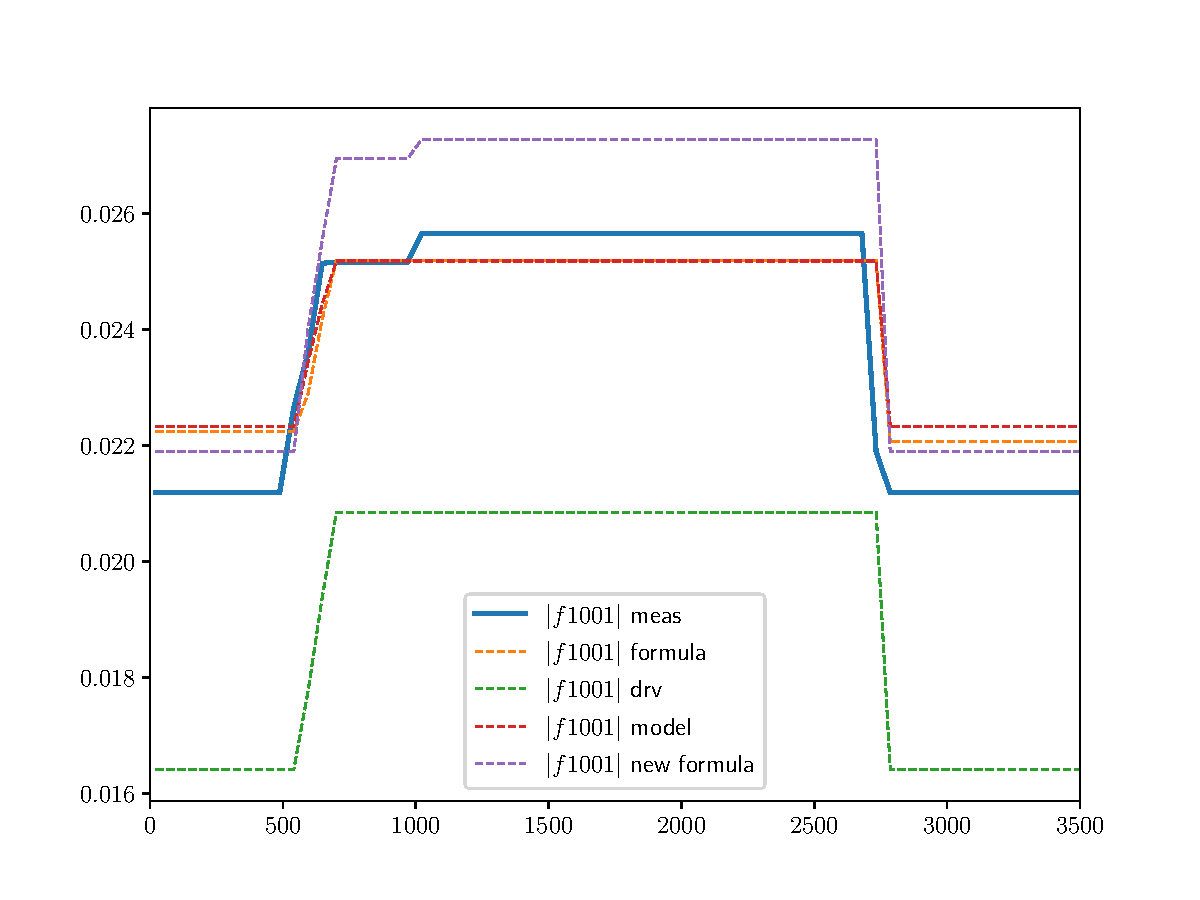
\includegraphics{forced_rdts_abs}
  \caption{Comparison of the three methods with the AC-dipole surrounded by a coupling bump.
    The AC-dipole is creating a jump in the coupling term $f_{1001}$ at its location. Only the new
    formula is able to reproduce this jump.
  }
  \label{fig_comp_felix_ryo}
\end{figure}
%
Figure~\ref{fig_comp_felix_ryo} shows the comparison between the three methods.



%\printindex

\bibliography{literature}
\bibliographystyle{thesis_bibstyle}
    
\end{document}
